\documentclass{article}

\usepackage[utf8]{inputenc}
\usepackage[italian]{babel}
\usepackage[T1]{fontenc}
\usepackage{lmodern}
\usepackage{graphicx}
\usepackage{caption}
\usepackage{amsmath, amssymb}
\usepackage{hyperref}
\usepackage{geometry}
\usepackage{enumitem}
\usepackage{booktabs}
\usepackage{float} % force figures and tables to appear exactly where declared
\usepackage{adjustbox}
\usepackage{svg}
\usepackage{multicol}
\usepackage[
    backend=biber,
    style=numeric,
    sorting=none,
]{biblatex}

\addbibresource{references.bib} %Import the bibliography file

\geometry{margin=1in}
\setlength{\columnsep}{0.5cm}

\newcommand{\myparagraph}[1]{\paragraph{#1}\mbox{}\\}

\title{Analisi e classificazione di abitudini di consumo di alcool e sigarette tramite tecniche di Machine Learning}
\author{%
  Marco Deano, matricola VR503057\\
  Marco Giacopuzzi, matricola VR509643\\[1ex]
  \textbf{Laurea magistrale in "Ingegneria e scienze informatiche"}\\
  \textbf{Anno accademico 2024/2025}\\
  \textbf{Corso di "Fondamenti di Machine Learning"}
}
\date{}

\begin{document}
\maketitle
\tableofcontents
\newpage

\begin{multicols}{2}

%%%%%%%%%%%%%%%%%%%%%%%%%%%%%%%%%%%%%%%%%%%%%%%%%%%%%%%%%%%%%%%%%%%%%
\section{Dataset e Obiettivi}
%%%%%%%%%%%%%%%%%%%%%%%%%%%%%%%%%%%%%%%%%%%%%%%%%%%%%%%%%%%%%%%%%%%%%

\subsection{Presentazione del dataset}

Il dataset tabellare utilizzato in questo progetto è composto da circa 1 milione di righe e 24 caratteristiche che contengono informazioni su vari parametri clinici e/o anagrafici degli individui; Le caratteristiche presenti includono sia dati numerici (misure biometriche) che variabili categoriali (genere).~\cite{sooyoungher_smoking_drinking}

Le etichette di classificazione considerate nel presente studio sono due:

\begin{itemize}[leftmargin=*]
    \item \textit{Bevitore} / \textit{Non bevitore} $\rightarrow$ problema di classificazione binaria;
    \item \textit{Fumatore} / \textit{Ex fumatore} / \textit{Non fumatore} $\rightarrow$ problema di classificazione multiclasse.
\end{itemize}

Il dataset presenta uno sbilanciamento nelle classi relative al fumo, con una distribuzione approssimativa del 60\% di non fumatori, 15\% di ex-fumatori e 25\% di fumatori attuali.
Al contrario, la distribuzione delle classi relative al consumo di alcol è bilanciata, con una divisione pari al 50\% tra bevitori e non bevitori. (Figura~\ref{fig:class_distribution})

\begin{figure*}[!htb] % Spans both columns and tries to place exactly where declared
  \centering
  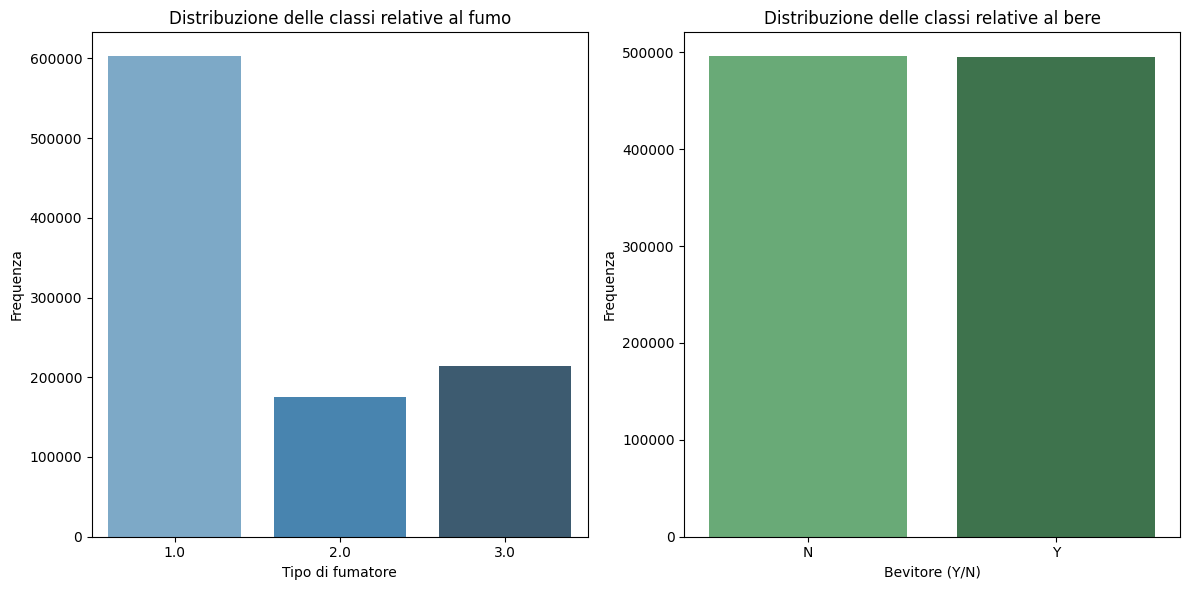
\includegraphics[width=0.8\textwidth]{screen_results/classes_distribution.png}
  \caption{Distribuzione delle classi}
  \label{fig:class_distribution}
\end{figure*}

Abbiamo deciso di lavorare con questo dataset per diversi motivi:
\begin{enumerate}[leftmargin=*]
    \item \textbf{Dimensioni del dataset e sua struttura:} 
    Essendo un dataset contenente quasi 1 milione di sample, ed essendo ben strutturato con delle feature chiare ed esplicite, abbiamo ritenuto fosse adatto per simulare una situazione reale in cui viene richiesto di risolvere una task di classificazione a partire dai parametri clinici dei pazienti. 
    Il dataset proviene da un sito governativo Coreano, che ne attesta l'autenticit\`a.~\cite{data_go_kr} 
    Il contenuto si \`e rivelato da subito chiaro e comprensibile e non sono state necessarie operazioni di pre-processing particolarmente complesse.
    
    \item \textbf{Tipologia di dataset:} 
    Riteniamo che l'impiego delle diverse tecniche di Machine Learning rappresenti un importante strumento applicabile a una vasta gamma di ambiti, come quello medico.
    
    Sebbene questo dataset non sia stato raccolto con l'intento di applicarvi tecniche di intelligenza artificiale, la possibilità di sviluppare un modello di Machine Learning in grado di determinare, con un certo grado di confidenza, il rapporto del paziente con fumo ed alcool si è subito rivelata stimolante.

    Nel contesto del ricovero ospedaliero, potrebbe risultare cruciale conoscere il rapporto del paziente con l'alcool e con il fumo.
    Non è da escludere che il paziente possa omettere informazioni o decidere di non rispondere in merito a tali abitudini: uno strumento in grado di fornire indicazioni circa questi aspetti, risulterebbe senz'altro utile.
    
    \item \textbf{Obiettivo del progetto non banale:} 
    
    Nonostante il dataset preveda una classificazione in sole tre classi per quanto riguarda il fumo e una classificazione binaria per l'alcool, riteniamo che il compito di classificare un paziente come "Fumatore", "Ex-fumatore" o "Non fumatore" non sia affatto banale: sono infatti diverse le situazioni che possono contrastare questo compito.

    Non possiamo sapere con assoluta certezza per quanto tempo i pazienti hanno smesso di fumare, con quale frequenza lo fanno o se i loro parametri clinici sono diversi a causa di altre malattie. Come si potr\`a osservare durante lo sviluppo del progetto, abbiamo impiegato molta energia nel cercare di ottimizzare quanto più possibile la previsione per il caso del fumo siccome si è rivelato un compito più impegnativo si quanto preventivato.


    
\end{enumerate}

\subsection{Obiettivo del progetto}

L'obiettivo principale del progetto è:

\begin{itemize}[leftmargin=*]
    \item Creare un modello che cerchi di classificare correttamente il maggior numero possibile di sample sia per il caso del fumo che dell'alcool;
\end{itemize}

Cercheremo di raggiungere questo obiettivo per fasi, iniziando con modelli più semplici e proseguendo con approcci più complessi o, comunque, diversi dal punto di vista metodologico.

Durante tutto lo svolgimento del progetto, monitoreremo costantemente i risultati delle predizioni dei vari modelli, con l'intento di migliorarli progressivamente.

%%%%%%%%%%%%%%%%%%%%%%%%%%%%%%%%%%%%%%%%%%%%%%%%%%%%%%%%%%%%%%%%%%%%%
\section{State of the Art (accenni)}
%%%%%%%%%%%%%%%%%%%%%%%%%%%%%%%%%%%%%%%%%%%%%%%%%%%%%%%%%%%%%%%%%%%%%

L'analisi di dataset inerenti l'ambito medico e la creazione di modelli utili per la diagnosi di malattie e non solo, è un tema ampiamente studiato nell'ambito del Machine Learning. Attualmente, i modelli più utilizzati per problemi di classificazione in questo contesto sono sicuramente:

\begin{itemize}[leftmargin=*]
    \item \textbf{Decision Tree} e \textbf{Random Forest}: noti per la loro robustezza agli outlier e per la capacità di gestire feature categoriali e numeriche senza necessità di encoding e scalatura.
    \item \textbf{Support Vector Machine}: efficaci in scenari con alta dimensionalità, specialmente con l'uso di kernel non lineari.
    \item \textbf{Reti neurali}: modelli molto più complessi rispetto a quelli tradizionali di Machine Learning, ma spesso richiedono dataset molto grandi.
\end{itemize}

Tuttavia, questi modelli non possono essere applicati senza una selezione ragionata e sensata degli iperparametri e delle feature da utilizzare. Le criticità a cui si rischia di andare incontro includono:

\begin{itemize}[leftmargin=*]
    \item \textbf{Sbilanciamento delle classi}: nei dataset reali, come quello preso in esame, alcune classi (es. ex-fumatori) possono essere sottorappresentate, portando a bias nei modelli.
    \item \textbf{Feature selection}: non tutte le feature presenti nel dataset sono necessariamente informative e importanti per la classificazione, e l'inclusione di quelle irrilevanti può peggiorare le performance.
    \item \textbf{Scelta degli iperparametri}: la selezione ottimale di parametri come la profondità degli alberi in Random Forest, il tipo di kernel in SVM o ancora il numero di "neighbours" in modelli tipo K-NN, influisce significativamente sulla qualità del modello.
\end{itemize}

%%%%%%%%%%%%%%%%%%%%%%%%%%%%%%%%%%%%%%%%%%%%%%%%%%%%%%%%%%%%%%%%%%%%%
\section{Metodologie, Modelli ed Algoritmi utilizzati}
%%%%%%%%%%%%%%%%%%%%%%%%%%%%%%%%%%%%%%%%%%%%%%%%%%%%%%%%%%%%%%%%%%%%%

I risultati e le performance dei modelli utilizzati durante i vari esperimenti sono stati monitorati tenendo in considerazione le metriche tradizionali di \textit{Accuratezza}, \textit{Precisione}, \textit{Recall} ed \textit{F1-score}, con particolare attenzione all'\textit{Accuratezza} nel contesto della classificazione binaria dell'alcool e all'\textit{F1-score} per la classificazione multiclasse del fumo. 
Per quanto riguarda il caso multiclasse, la scelta di basarsi su \textit{F1-score} è stata determinata dalla sua utilità nel trattare problemi caratterizzati da uno sbilanciamento delle classi, poiché questa metrica bilancia efficacemente precisione e recall.
Inoltre, l'uso dell'\textit{F1-score} aiuta a prevenire situazioni in cui un modello sembri performante semplicemente perché predice con successo la classe maggioritaria, mentre un buon valore di \textit{F1-score} indica che il modello riconosce correttamente anche le classi meno rappresentate. 

Parallelamente, l'impiego delle \textit{Confusion Matrix} si è rivelato essenziale per la valutazione del modello durante l'intero progetto.

Come sarà dettagliato nel prosieguo, durante i progetto sono stati testati diversi modelli di Machine Learning con l'intento di identificare quello pi\`u idoneo per il nostro problema di classificazione. 
Non ci siamo limitati alla valutazione dei modelli di base, ma abbiamo integrato ogni fase con l'adozione di tecniche supplementari volte a migliorare la qualità dei dati in ingresso e a ottimizzare le performance complessive dei modelli. 

Sono state impiegate, variando a seconda del modello utilizzato, le seguenti tecniche:

\begin{itemize}[leftmargin=*]
    \item \textbf{Feature selection:}
    al fine di ridurre la dimensionalità del dataset e migliorare l'efficienza generale dei modelli.
    
    \item \textbf{Feature engineering:} 
    in parallelo alla selezione delle feature, sono state create, trasformate e ottimizzate le caratteristiche del dataset per migliorarne le performance. 
    In particolare, sono state condotte ricerche specifiche sul dominio di studio, per creare nuove feature in grado di arricchire il dataset iniziale, con l'obiettivo di migliorare le performance predittive dei modelli.
    
    \item \textbf{Ottimizzazione degli iperparametri:} 
    attraverso l'uso della tecnica di "Grid Search" sono state testate, per ciascun modello, differenti combinazioni di iperparametri, al fine di individuare la configurazione migliore per il nostro problema.
    
    \item \textbf{Principal Component Analysis:} 
    per ridurre la dimensionalità del dataset mantenendo la varianza massima. 
    Per molti modelli l'applicazione a monte di PCA, con una conseguente riduzione del rumore, pu\`o  concretizzarsi in un miglioramento delle prestazioni predittive.
    
    \item \textbf{Tecniche di ensemble prediction:} 
    in presenza di dataset di grandi dimensioni, l'utilizzo di un singolo modello potrebbe non rappresentare la soluzione più adeguata, rischiando di predire correttamente solo alcune classi e non altre. 
    Per questo motivo, sono state adottate tecniche di ensemble prediction (quali bagging, boosting e stacking) per ottenere predizioni più robuste e affidabili.
    
    \item \textbf{Classificazione gerarchica:} 
    un ulteriore approccio adottato è stato l'introduzione di una strategia di classificazione gerarchica, particolarmente utile per affrontare il problema dello sbilanciamento delle classi, con particolare riferimento alla task di classificazione del fumo.
    
\end{itemize}


\subsection{Preprocessing e Pulizia del Dataset}

Prima di applicare qualsiasi modello di Machine Learning, è fondamentale assicurarsi che il dataset non presenti criticit\`a nei dati (e.g. valori null/Nan, outliers, campi categorici, etc\dots) ed eventualmente risolverle per poter sfruttare al meglio le potenzialità dei vari modelli di apprendimento.
Abbiamo dunque seguito i seguenti passaggi:

\begin{enumerate}[leftmargin=*]
    \item \textbf{Analisi preliminare del dataset}:
    abbiamo effettuato un'analisi del dataset ed estrapolato tutte le informazioni utili per comprenderne la struttura.
    Nello specifico, tramite semplici script, abbiamo:
    \begin{itemize}[leftmargin=*]
        \item Calcolato la distribuzione dei valori per le varie feature;
        \item Analizzato la distribuzione delle classi nel dataset;
        \item Tracciato boxplot per individuare la presenza di eventuali outlier che potrebbero interferire con il training dei modelli (Figura~\ref{fig:feature_boxplots}).
    \end{itemize}
    
    \item \textbf{Identificazione e rimozione degli outlier}:
    l'analisi del dataset ha permesso di individuare facilmente molti degli outlier più evidenti (e.g. valori estremamente distanti dalla media e probabilmente sbagliati) ed eliminarli.
    Successivamente alla eliminazione dei sample contenenti errori sono state rimosse tramite \textbf{Z-score} le code delle distribuzioni rappresentative di casi clinici particolari che potrebbero influenzare negativamente le performance dei modelli.~\cite{zscore}
    
    \item \textbf{Encoding delle variabili categoriali}:
    abbiamo applicato il \textbf{Label Encoding} per le variabili categoriali.
    Non è stato necessario utilizzare il \textbf{One-Hot Encoding}, poiché le uniche feature categoriali presenti sono \textit{sex} e le label delle classi.
\end{enumerate}

Lo \textbf{scaling} dei dati è stato applicato prima dell'utilizzo dei modelli che ne beneficiano: sono presenti infatti features con valori su scale diverse.

Una delle ipotesi iniziali prevedeva di utilizzare le ground truth di \textit{smoke} come feature per la classificazione di \textit{drink} (e viceversa).
Dopo alcuni test preliminari, visti gli scarsi miglioramenti, questa strada è stata abbandonata.

%%%%%%%%%%%%%%%%%%%%%%%%%%%%%%%%%%%%%%%%%%%%%%%%%%%%%%%%%%%%%%%%%%%%%
\subsection{Un primo esempio con un modello semplice}
%%%%%%%%%%%%%%%%%%%%%%%%%%%%%%%%%%%%%%%%%%%%%%%%%%%%%%%%%%%%%%%%%%%%%

Una volta terminata la fase di analisi e pulizia dei dati, abbiamo testato un modello base, utilizzando un classificatore semplice come un \textit{Logistic Regressor}, per ottenere un primo benchmark sulle performance e dopo aver analizzato questi primissimi risultati, abbiamo gradualmente introdotto modelli più complessi e implementato diverse tecniche di ottimizzazione per migliorare le prestazioni.

\begin{figure*}[!htb]
  \centering
  \includesvg[width=0.9\textwidth]{screen_results/boxplot_feature.svg}
  \caption{Boxplot per Features}
  \label{fig:feature_boxplots}
\end{figure*}


%%%%%%%%%%%%%%%%%%%%%%%%%%%%%%%%%%%%%%%%%%%%%%%%%%%%%%%%%%%%%%%%%%%%%
\subsection{Random Forest}
%%%%%%%%%%%%%%%%%%%%%%%%%%%%%%%%%%%%%%%%%%%%%%%%%%%%%%%%%%%%%%%%%%%%%

Abbiamo inizialmente testato un modello base di Random Forest, senza esplicitare i valori dei vari iperparametri, per ottenere dei primi risultati di riferimento e comprendere il comportamento del modello sui nostri dati; dopo aver valutato le metriche di performance, ci siamo resi conto che c'erano margini di miglioramento e abbiamo deciso di affinare il modello seguendo un approccio progressivo.

Per prima cosa, abbiamo proceduto con un’ottimizzazione degli iperparametri sfruttando una "Grid Search" per affinare ulteriormente la ricerca; tra i parametri più rilevanti abbiamo considerato il numero di alberi nella foresta, la profondità massima degli alberi e il numero minimo di campioni richiesti per effettuare uno split dei nodi, tenendo sempre monitorati tutte le metriche citate prima ma prestando particolare attenzione all'F1-score. Ci siamo subito accorti che, solo facendo una ricerca degli iperparametri ottimali, le metriche cominciavano a migliorare e la confusion matrix diventava sempre più bilanciata, con una riduzione degli errori di classificazione soprattutto nelle classi meno rappresentate; inoltre la confusion matrix ci ha permesso di individuare quali classi venivano maggiormente confuse tra loro, aiutandoci a comprendere dove il modello faticava maggiormente

A questo punto, abbiamo provato ad ottimizzare la RandomForest sfruttando la tecnica della feature selection: avendo a che fare con un modello predittivo di questo tipo, ovvero abbastanza robusto alle feature irrilevanti, non ci aspettavamo un grosso miglioramento delle performance ma nonostante ciò rimane comunque un passaggio utile per poter eventualmente semplificare il modello andando a togliere anche poche feature e rendere il modello predittivo più veloce. Inoltre, non è stato indicato a priori un numero fissato di feature da selezionare, in quanto non certi di quelle che potessero essere le performance selezionando solo il 10\%, il 20\%, il 50\%, il 75\%... delle feature; quindi abbiamo implementato un algoritmo di feature selection di tipo Forward, monitorando la F1-score ad ogni "best\_feature" aggiunta, e salvando la combinazione di feature migliore tra tutte quelle testate.

Per validare ulteriormente il nostro approccio, abbiamo infine applicato la cross-validation utilizzando la tecnica \textsc{StratifiedKFold}, in modo da avere una valutazione più affidabile delle performance su diverse suddivisioni del dataset: siccome nello step precedente in cui abbiamo effettuato feature selection abbiamo allenato il nostro modello tenendo costante il set di train e di validazione, potremmo aver "overfittato" in base alla suddivisione specifica; con la cross-validation, testiamo il modello su diverse porzioni del dataset e possiamo valutare se le feature scelte hanno migliorato davvero il modello.

Dopo tutte queste analisi, la Random Forest si è dimostrata un modello solido, in grado di ottenere buoni risultati con un tempo di addestramento contenuto; inoltre, come si è potuto evincere, non si sono rese necessarie operazioni come Scaling dei dati o Dimensionality Reduction e questo perchè il modello Random Forest non è influenzato da grandezze diverse tra le feature e gestisce bene dati ad alta dimensionalità.

\subsubsection*{Valori selezionati per gli iperparametri}

\begin{itemize}[leftmargin=*]
    \item n\_estimators=100
    \item max\_depth=20
    \item min\_samples\_split=50
\end{itemize}

%%%%%%%%%%%%%%%%%%%%%%%%%%%%%%%%%%%%%%%%%%%%%%%%%%%%%%%%%%%%%%%%%%%%%
\subsection{Altri Classificatori}
%%%%%%%%%%%%%%%%%%%%%%%%%%%%%%%%%%%%%%%%%%%%%%%%%%%%%%%%%%%%%%%%%%%%%

Ovviamente non ci siamo limitati ad utilizzare ed ottimizzare solamente il modello di Random Forest, ma abbiamo effettuato le stesse procedure anche con modelli totalmente differenti nella loro filosofia. Nel progetto non sono stati riportati tutti questi passaggi per evitare di appesantire troppo la trattazione, tuttavia abbiamo incluso tutti i risultati per evidenziare le differenze di performance tra i vari approcci e giustificare le scelte effettuate.

I modelli allenati e testati sono stati:

\begin{itemize}[leftmargin=*]
    \item \textbf{KNN}: rappresenta un metodo basato sulla similarità tra i dati, permettendoci di analizzare il comportamento del modello quando la decisione dipende strettamente dalla vicinanza ai punti nel dataset. Questo modello è particolarmente utile poiché non richiede alcuna assunzione sui dati e consente di costruire confini di classificazione non lineari. Di conseguenza, ci ha permesso di valutare se le classi fossero separabili nello spazio delle feature disponibili.
    
    \item \textbf{AdaBoost (con base\_estimator Albero Decisionale)}: un modello di ensemble basato sul boosting, noto per la sua capacità di concentrarsi sugli errori commessi dai modelli più deboli nelle iterazioni precedenti, migliorando progressivamente la qualità della classificazione. Abbiamo deciso di testare questo modello per verificare se un metodo di ensemble focalizzato su un raffinamento iterativo potesse fornire risultati migliori rispetto a un metodo più stabile come Random Forest.
    
    \item \textbf{Support Vector Machine (kernel lineare)}: è un modello molto efficace nei problemi di classificazione, in particolare quando i dati sono ben separabili in uno spazio ad alta dimensione. Nonostante sapessimo che difficilmente i sample del nostro dataset lo sarebbero stati, abbiamo deciso di testare questo modello per verificare empiricamente se una SVM con kernel lineare potesse individuare un iperpiano di separazione efficace, grazie all’uso di margini ampi e alla capacità di gestire outlier tramite il parametro di penalizzazione.
\end{itemize}

Prima di allenare questi modelli, ci siamo assicurati di normalizzare i dati di train e test per ottenere le migliori performance possibili.

Oltre a testare questi modelli nella loro versione base e con iperparametri ottimizzati, abbiamo anche valutato l'applicazione della \textit{Principal Component Analysis} (PCA) come tecnica di riduzione della dimensionalità. Questa tecnica è stata applicata solo ai modelli KNN e SVM, mentre per il modello AdaBoost con base\_estimator Albero Decisionale abbiamo ritenuto che non fosse necessaria. Dato che il dataset dispone di 22 feature e che avevamo già testato la tecnica della selezione delle feature, volevamo valutare se la riduzione della dimensionalità tramite PCA potesse migliorare le prestazioni dei modelli. 

Per quanto riguarda l’utilizzo della PCA, non abbiamo creato un notebook contenente tutti i passaggi per selezionare il miglior numero di componenti da passare come parametro alla PCA. Abbiamo invece riportato direttamente la versione che ha permesso di ottenere i migliori risultati.

\subsubsection*{Valori selezionati per gli iperparametri}

\begin{itemize}[leftmargin=*]
    \item AdaBoostClassifier(n\_estimators=200)
    \item LinearSVC(C=0.1)
    \item KNeighborsClassifier(n\_neighbors=500)
\end{itemize}


%%%%%%%%%%%%%%%%%%%%%%%%%%%%%%%%%%%%%%%%%%%%%%%%%%%%%%%%%%%%%%%%%%%%%
\subsection{Feature Engineering}
%%%%%%%%%%%%%%%%%%%%%%%%%%%%%%%%%%%%%%%%%%%%%%%%%%%%%%%%%%%%%%%%%%%%%

Una volta testati tutti i modelli predittivi di Machine Learning, sono state condotte delle ricerche inerenti il dominio trattato in questo progetto, con l'obiettivo di creare nuove feature. Tali feature sono state progettate per generare un dataset arricchito, con parametri differenti rispetto a quelli inizialmente disponibili. L'intento principale di questa fase è stato quello di migliorare le performance dei modelli predittivi, estraendo informazioni più significative dalle feature esistenti o creando nuove caratteristiche che potessero contribuire a ottimizzare le performance dei classificatori.

\subsubsection{Caratteristiche Antropometriche}

Le caratteristiche antropometriche rappresentano buoni indicatori dello stato fisico di un paziente, parametri che possono essere influenzati dal fumo e dal consumo di alcol. L'obesità e la distribuzione anomala del grasso sono condizioni frequentemente correlate a comportamenti a rischio e possono essere identificate attraverso questi parametri.

\begin{itemize}[leftmargin=*]
    \item \textbf{BMI}: Misura l'obesità generale.
    \item \textbf{wth\_ratio}: Rapporto vita/altezza, indica l'obesità addominale.
    \item \textbf{wtw\_ratio}: Rapporto vita/peso, evidenzia la distribuzione del grasso.
    \item \textbf{obesity\_flag}: Flag per identificare rapidamente l'obesità.
\end{itemize}

\subsubsection{Caratteristiche Cardiovascolari}

Le caratteristiche cardiovascolari forniscono informazioni chiave sullo stato del sistema circolatorio, il quale può essere compromesso dal fumo e dal consumo di alcol. Questi parametri evidenziano anomalie pressorie e rigidità arteriosa, segnali indiretti di comportamenti a rischio.

\begin{itemize}[leftmargin=*]
    \item \textbf{pulse\_pressure}: Differenza tra SBP e DBP, indice di rigidità arteriosa.
    \item \textbf{MAP}: Misura globale della pressione arteriosa.
    \item \textbf{bp\_category}: Classifica la pressione, rilevando eventuali anomalie.
\end{itemize}

\subsubsection{Profilo Lipidico e Rapporti Metabolici}

Le caratteristiche metaboliche forniscono informazioni sullo stato cardiovascolare e metabolico dei pazienti. Esse offrono anche spunti su come il fumo e il consumo di alcol possano alterare questi parametri. Un profilo lipidico instabile e un disequilibrio nei rapporti metabolici possono essere indicatori indiretti di uno stile di vita malsano.

\begin{itemize}[leftmargin=*]
    \item \textbf{TC\_HDL\_ratio}: Indica il rischio cardiovascolare confrontando il colesterolo totale con l'HDL.
    \item \textbf{LDL\_HDL\_ratio}: Evidenzia lo squilibrio tra il colesterolo "cattivo" e quello "buono".
    \item \textbf{non\_HDL\_chole}: Misura le particelle aterogeniche, segnale di potenziali patologie.
    \item \textbf{triglyceride\_hdl\_ratio}: Riflette il rischio metabolico influenzato da dieta e stile di vita.
    \item \textbf{AIP}: Valuta sinteticamente il rischio cardiovascolare tramite il logaritmo di trigliceridi/HDL.
    \item \textbf{TyG}: Indica resistenza insulinica e rischio metabolico calcolando trigliceridi e glucosio.
\end{itemize}

\subsubsection{Funzione Epatica e Renale}

L'inclusione di indicatori per la funzione epatica e renale risulta vantaggiosa poiché i cambiamenti in questi parametri possono essere segnali indiretti di danni organici causati dal fumo e dal consumo di alcol. Questi indicatori aiutano a identificare stili di vita a rischio fornendo informazioni sullo stato degli organi.

\begin{itemize}[leftmargin=*]
    \item \textbf{AST\_ALT\_ratio}: Valori elevati possono indicare danni epatici da alcol.
    \item \textbf{liver\_enzyme\_interaction}: Segnala anomalie enzimatiche legate all'abuso di alcol.
    \item \textbf{liver\_enzyme\_avg}: Fornisce una panoramica rapida della funzione del fegato.
    \item \textbf{eGFR}: Utile per rilevare danni renali associati a stili di vita non salutari.~\cite{levey2009new}
\end{itemize}

Poiché l'aggiunta di queste nuove feature ha comportato un incremento della dimensionalità del dataset, è stato ritenuto opportuno applicare la tecnica di PCA. È importante sottolineare che è stata testata solo questa tecnica e non la \textit{Feature Reduction} successivamente all'aggiunta delle nuove feature, a causa delle limitazioni temporali per ottenere i risultati. L'utilizzo della PCA è stato considerato un test necessario per cercare di estrarre pattern più significativi, dato l'aumento del numero totale di feature nel dataset derivante dal processo di feature engineering.



%%%%%%%%%%%%%%%%%%%%%%%%%%%%%%%%%%%%%%%%%%%%%%%%%%%%%%%%%%%%%%%%%%%%%
\subsection{Bagging Ensemble}
%%%%%%%%%%%%%%%%%%%%%%%%%%%%%%%%%%%%%%%%%%%%%%%%%%%%%%%%%%%%%%%%%%%%%

Arrivati a questo punto del progetto non ci rimanevano molti modelli/tecniche da provare per migliorare i risultati già ottenuti, quindi una delle ultime tecniche di predizione che abbiamo testato è stata quella del bagging ensemble: una tecnica che consiste nel combinare i risultati ottenuti da più modelli per ottenere una predizione più accurata. I modelli che abbiamo utilizzato per fare bagging ensemble, sono stati AdaBoost e Support Vector Machine (kernel rbf), abbiamo scelto questi 2 modelli per le seguenti ragioni:

\begin{itemize}[leftmargin=*]
    \item Volevamo provare a fondere la tecnica del boosting (caratteristica di AdaBoost) con la tecnica del bagging ensemble
    \item Siccome il tempo per il training di un modello di SVM non lineare scala in maniera quadratica con il numero di sample, era proibitivo allenare un modello singolo di questo tipo anche solo utilizzando il 50\% del dataset (500.000 sample); dunque abbiamo optato per utilizzare la tecnica dell'ensemble utilizzando più modelli SVM non lineari ma allenati ognuno su una porzione ristretta del dataset.
\end{itemize}

Non abbiamo testato la tecnica del bagging ensemble per altri modelli come Random Forest perchè secondo il nostro parere non avrebbe apportato un beneficio significativo: nel caso della Random Forest il bagging è già un componente fondamentale del modello stesso in cui vengono costruiti più alberi su sottocampioni del dataset e poi aggregati tramite voto maggioritario, mentre per quanto riguarda KNN, il bagging non risulta particolarmente efficace perchè il suo comportamento dipende essenzialmente dalla scelta dei vicini più prossimi e dalla distanza utilizzata.

\subsubsection*{Valori selezionati per gli iperparametri}

\begin{itemize}[leftmargin=*]
    \item BaggingClassifier( estimator=SVC( kernel='rbf', C=1), n\_estimators=30, max\_samples=0.1 )
    \item BaggingClassifier( estimator=AdaBoostClassifier( n\_estimators=50), n\_estimators=100 )
\end{itemize}

%%%%%%%%%%%%%%%%%%%%%%%%%%%%%%%%%%%%%%%%%%%%%%%%%%%%%%%%%%%%%%%%%%%%%
\subsection{Stacking Classifier e Voting Classifier}
%%%%%%%%%%%%%%%%%%%%%%%%%%%%%%%%%%%%%%%%%%%%%%%%%%%%%%%%%%%%%%%%%%%%%

Altre 2 tecniche di ensemble che abbiamo testato, sono state lo \textbf{Stacking Classifier} e il \textbf{Voting Classifier}: entrambi i metodi mirano a combinare più modelli per ottenere una predizione finale più robusta, come nel caso del bagging e del boosting, ma con approcci differenti.

\paragraph{Stacking Classifier} sfrutta un livello aggiuntivo di apprendimento rispetto al bagging, in quanto i risultati dei singoli modelli base utilizzati vengono impiegati come input per un meta-modello, che impara a combinare le loro predizioni in modo ottimale. Abbiamo selezionato come modelli base tutti quelli che abbiamo sfruttato nei test precedenti (escluso il SVM lineare) e abbiamo utilizzato come meta-modello un SVM con kernel lineare. Questa scelta è stata fatta per un motivo semplice: il modello \textit{Random Forest} fino a questo momento è risultato il migliore e abbiamo ritenuto corretto sfruttarlo come modello base all'interno dello stacking piuttosto che come meta-modello finale, evitando di inserirlo in entrambe le posizioni per non ridurre la diversità del sistema di ensemble. La scelta del meta-modello è dunque ricaduta sul SVM lineare, vista la sua velocità di training e i comunque buoni risultati garantiti fino a questo punto del progetto.

\paragraph{Voting Classifier} segue un approccio più semplice: aggrega le predizioni dei vari modelli base attraverso una strategia di voto, che può essere di tipo \emph{hard voting} (sceglie la classe con più voti tra i modelli) o \emph{soft voting} (media delle probabilità predette).

%%%%%%%%%%%%%%%%%%%%%%%%%%%%%%%%%%%%%%%%%%%%%%%%%%%%%%%%%%%%%%%%%%%%%
\subsection{Classificatore Gerarchico}
%%%%%%%%%%%%%%%%%%%%%%%%%%%%%%%%%%%%%%%%%%%%%%%%%%%%%%%%%%%%%%%%%%%%%

Arrivati a questo punto del progetto, ci siamo resi conto che l'obiettivo di separare in maniera sempre più precisa la classe dei Fumatori da quella degli Ex-fumatori e da quella dei Non-fumatori risultava particolarmente complesso a causa dello sbilanciamento delle classi e della possibile sovrapposizione nei pattern dei dati. 
Ci siamo accorti però che tutti i modelli allenati e perfezionati fino ad ora, avevano una cosa in comune: non riuscivano a separare correttamente la classe degli Ex-fumatori da quella dei Fumatori. 
Facendo poi un'analisi ancora più approfondita dei risultati, in particolar modo delle matrici di confusione ottenute, ci siamo però accorti che uno dei modelli testati nel progetto riusciva piuttosto bene a non classificare i Non Fumatori rispetto ai Fumatori o Ex-fumatori. 
Si tratta del modello Random Forest.

\begin{center}
    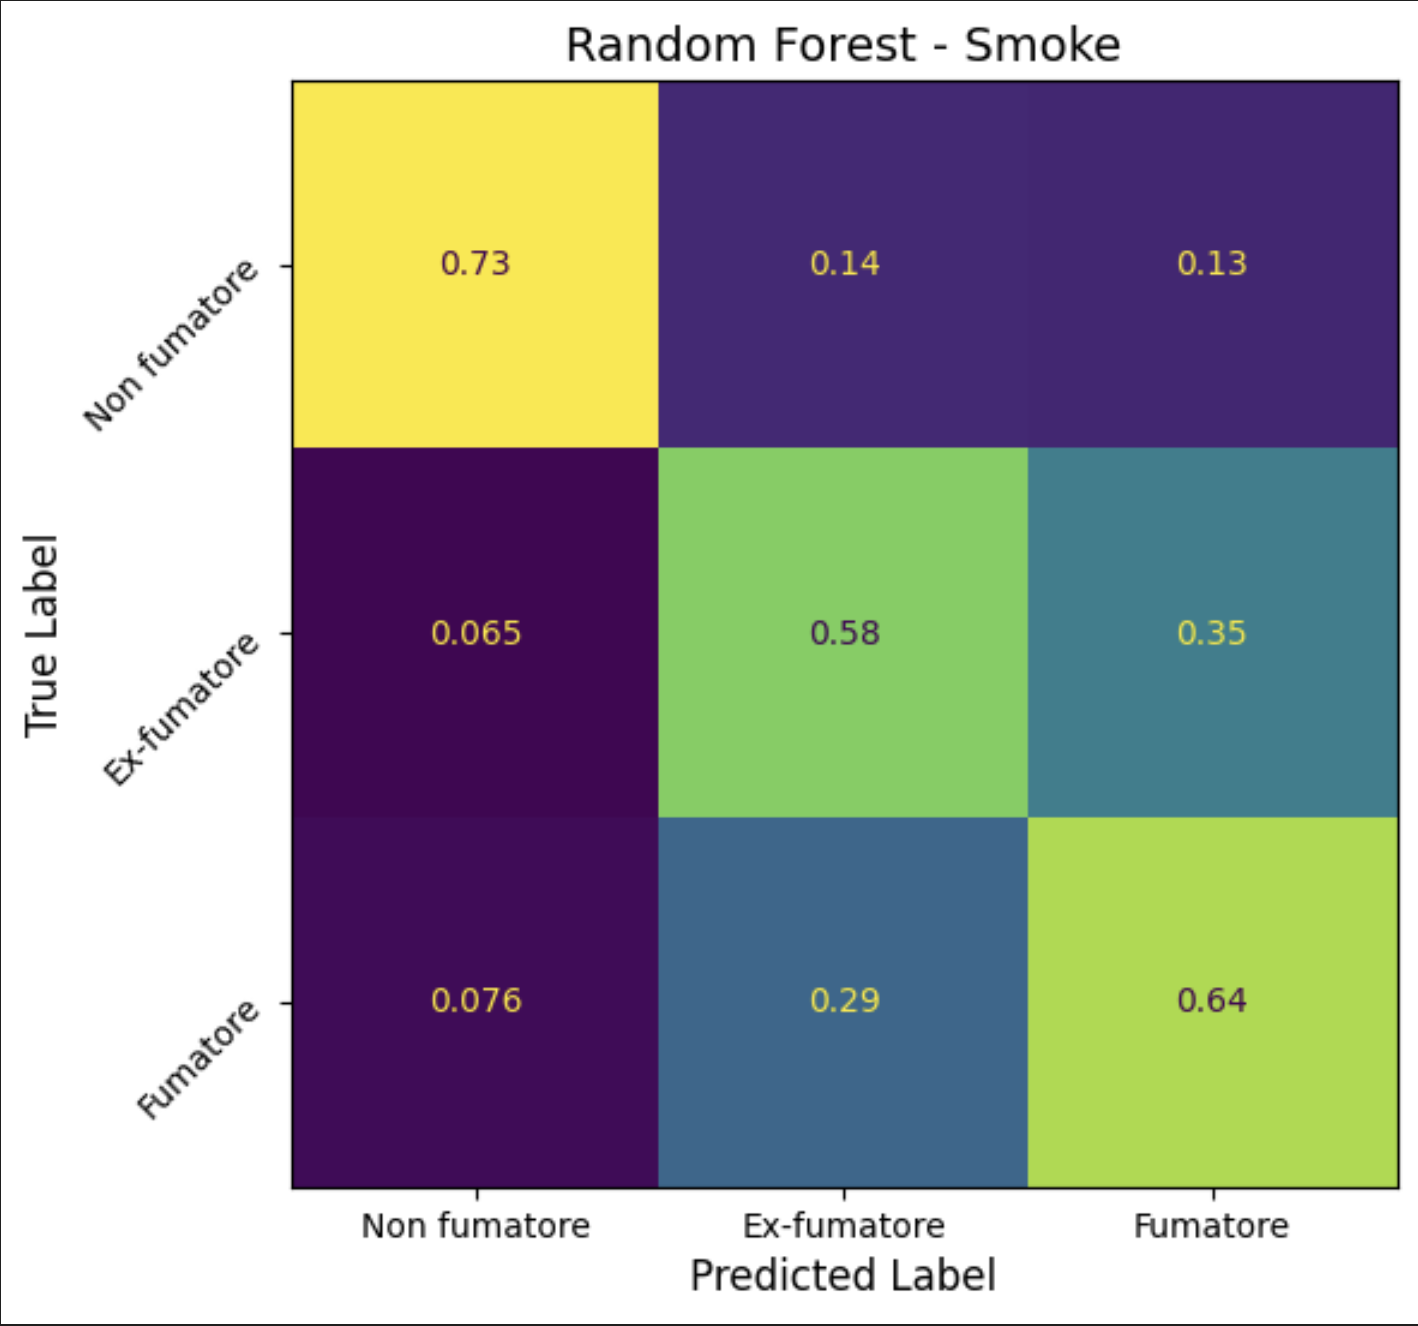
\includegraphics[width=0.75\columnwidth]{screen_results/confusion_matrix_rf_optimized_s.png}
\end{center}

Abbiamo quindi deciso di fare un ultimo tentativo per cercare di migliorare i risultati ottenuti fino a questo punto del progetto, sperimentando un approccio gerarchico alla classificazione e suddividendo il problema in due fasi distinte.

\begin{itemize}[leftmargin=*]
    \item \textbf{Primo classificatore:} un modello iniziale per distinguere tra Non-fumatori e la classe unificata Ex-fumatori + Fumatori.
    \item \textbf{Secondo classificatore:} un modello specifico addestrato per separare i campioni precedentemente classificati come Ex-fumatori + Fumatori, suddividendoli nelle due classi originali.
\end{itemize}

L'idea alla base di questa strategia è che venga allenato un primo modello in modo che possa distinguere chi non ha mai fumato da chi, invece, ha avuto un'esposizione al fumo e successivamente venga allenato un secondo classificatore che può invece concentrarsi sulla separazione tra Ex-fumatori e Fumatori attuali, che presentano differenze più sottili e meno evidenti rispetto alla distinzione con i Non-fumatori. 
Abbiamo dunque fatto una ricerca su quello che potesse essere un primo modello ottimale che potesse distinguere la classe dei Non-fumatori e la classe unificata Ex-fumatori + Fumatori e di seguito una ricerca analoga per selezionare il secondo modello. 
I nostri test hanno evidenziato come il miglior modello per riuscire a separare i Non-fumatori dalla classe unificata Ex-fumatori + Fumatori è lo Stacking Classifier, mentre per quanto riguarda il secondo modello il migliore in grado di separare Ex-fumatori e Fumatori è la Random Forest. 
Anche lo Stacking Classifier si avvicina molto come performance.

Nonostante l'idea di partenza ci sembrasse buona, ci siamo però accorti di quanto non fosse banale costruire un classificatore di questo tipo. 
Il fatto che il primo modello potesse classificare erroneamente dei sample con label "Non-fumatore" come "Ex-fumatore o Fumatore" e che poi dovessero essere classificati come "Ex-fumatore" o "Fumatore" ci ha creato dei grossi problemi nella creazione del modello che avevamo in mente noi. 
Difatti alla fine siamo stati costretti ad allenare il secondo modello con tutte e tre le label iniziali e non solo sulle label di "Ex-fumatore" e "Fumatore" come avevamo in mente all'inizio. 
Un'altra alternativa che ci era venuta in mente, è stata quella di allenare due modelli totalmente separati (il primo con label "Non-fumatore" e "Ex-fumatore o Fumatore" ed il secondo con label "Ex-fumatore" e "Fumatore") con una porzione del dataset, e in un secondo momento utilizzare il restante dataset come test. 
Non abbiamo implementato questa alternativa per il semplice motivo che non sarebbe stato possibile avere dei risultati direttamente comparabili con quelli ottenuti fino a questo punto.


%%%%%%%%%%%%%%%%%%%%%%%%%%%%%%%%%%%%%%%%%%%%%%%%%%%%%%%%%%%%%%%%%%%%%
\subsection{Visualizzazione Dati tramite t-SNE}
%%%%%%%%%%%%%%%%%%%%%%%%%%%%%%%%%%%%%%%%%%%%%%%%%%%%%%%%%%%%%%%%%%%%%

Per farci un'idea più generale di quello che potesse essere la distribuzione nello spazio dei dati presenti nel dataset, abbiamo anche sfruttato la tecnica di t-SNE; in questo modo abbiamo potuto visualizzare quanto effettivamente le classi del nostro dataset fossero sovrapposte tra di loro.
Ovviamente per rendere il tutto più comprensibile, abbiamo "plottato" il tutto in uno spazio a 2 dimensioni e considerando in un primo test le label "Non-fumatore" e "Ex-fumatore o Fumatore" accorpate in una unica classe ed in un secondo test le classi "Ex-fumatore" e "Fumatore".

\end{multicols}

\newpage

%%%%%%%%%%%%%%%%%%%%%%%%%%%%%%%%%%%%%%%%%%%%%%%%%%%%%%%%%%%%%%%%%%%%%
\section{Risultati}
%%%%%%%%%%%%%%%%%%%%%%%%%%%%%%%%%%%%%%%%%%%%%%%%%%%%%%%%%%%%%%%%%%%%%

In questa sezione vengono riportati i risultati dei diversi modelli di classificazione testati, vengono confrontate le loro prestazioni utilizzando le metriche citate nella sezione relativa agli obiettivi del progetto e vengono riportate le confusion matrix per comprendere meglio come mai alcuni modelli risultano essere migliori di altri.

%%%%%%%%%%%%%%%%%%%%%%%%%%%%%%%%%%%%%%%%%%%%%%%%%%%%%%%%%%%%%%%%%%%%%%%%%%%%%%
% Modello semplice Logistic Regression
%%%%%%%%%%%%%%%%%%%%%%%%%%%%%%%%%%%%%%%%%%%%%%%%%%%%%%%%%%%%%%%%%%%%%%%%%%%%%%

\subsection{Modello semplice Logistic Regression}

\subsection*{Smoke}
\begin{center}
\begin{minipage}[c]{0.50\columnwidth}
\resizebox{\columnwidth}{!}{%
\begin{tabular}{lcccc}
\toprule
Label        & Precision & Recall & F1-score & Support \\
\midrule
Non-smoker   & 0.69      & 0.91   & 0.79     & 167528 \\
Ex-smoker    & 0.40      & 0.09   & 0.15     & 47377  \\
Smoker       & 0.50      & 0.36   & 0.42     & 58574  \\
\midrule
Accuracy     & --        & --     & 0.65     & 273479 \\
Macro avg    & 0.53      & 0.45   & 0.45     & 273479 \\
Weighted avg & 0.60      & 0.65   & 0.60     & 273479 \\
\bottomrule
\end{tabular}%
}
\end{minipage}\hspace{\columnsep}%
\begin{minipage}[c]{0.40\columnwidth}
\centering
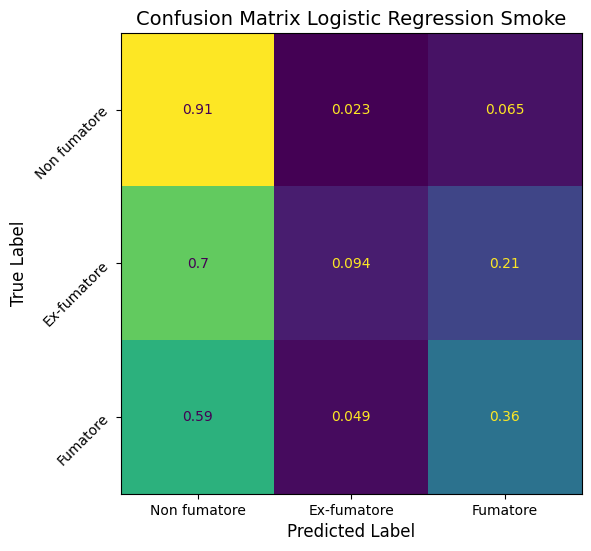
\includegraphics[width=\columnwidth,height=0.75\columnwidth,keepaspectratio]{screen_results/confusion_matrix_first_example_s.png}
\end{minipage}
\end{center}

\subsection*{Drink}
\begin{center}
\begin{minipage}[c]{0.50\columnwidth}
\resizebox{\columnwidth}{!}{%
\begin{tabular}{lcccc}
\toprule
Label  & Precision & Recall & F1-score & Support \\
\midrule
Y      & 0.70      & 0.70   & 0.70     & 135539 \\
N      & 0.71      & 0.70   & 0.70     & 137940 \\
\midrule
Accuracy     & --        & --     & 0.70     & 273479 \\
Macro avg    & 0.70      & 0.70   & 0.70     & 273479 \\
Weighted avg & 0.70      & 0.70   & 0.70     & 273479 \\
\bottomrule
\end{tabular}%
}
\end{minipage}\hspace{\columnsep}%
\begin{minipage}[c]{0.40\columnwidth}
\centering
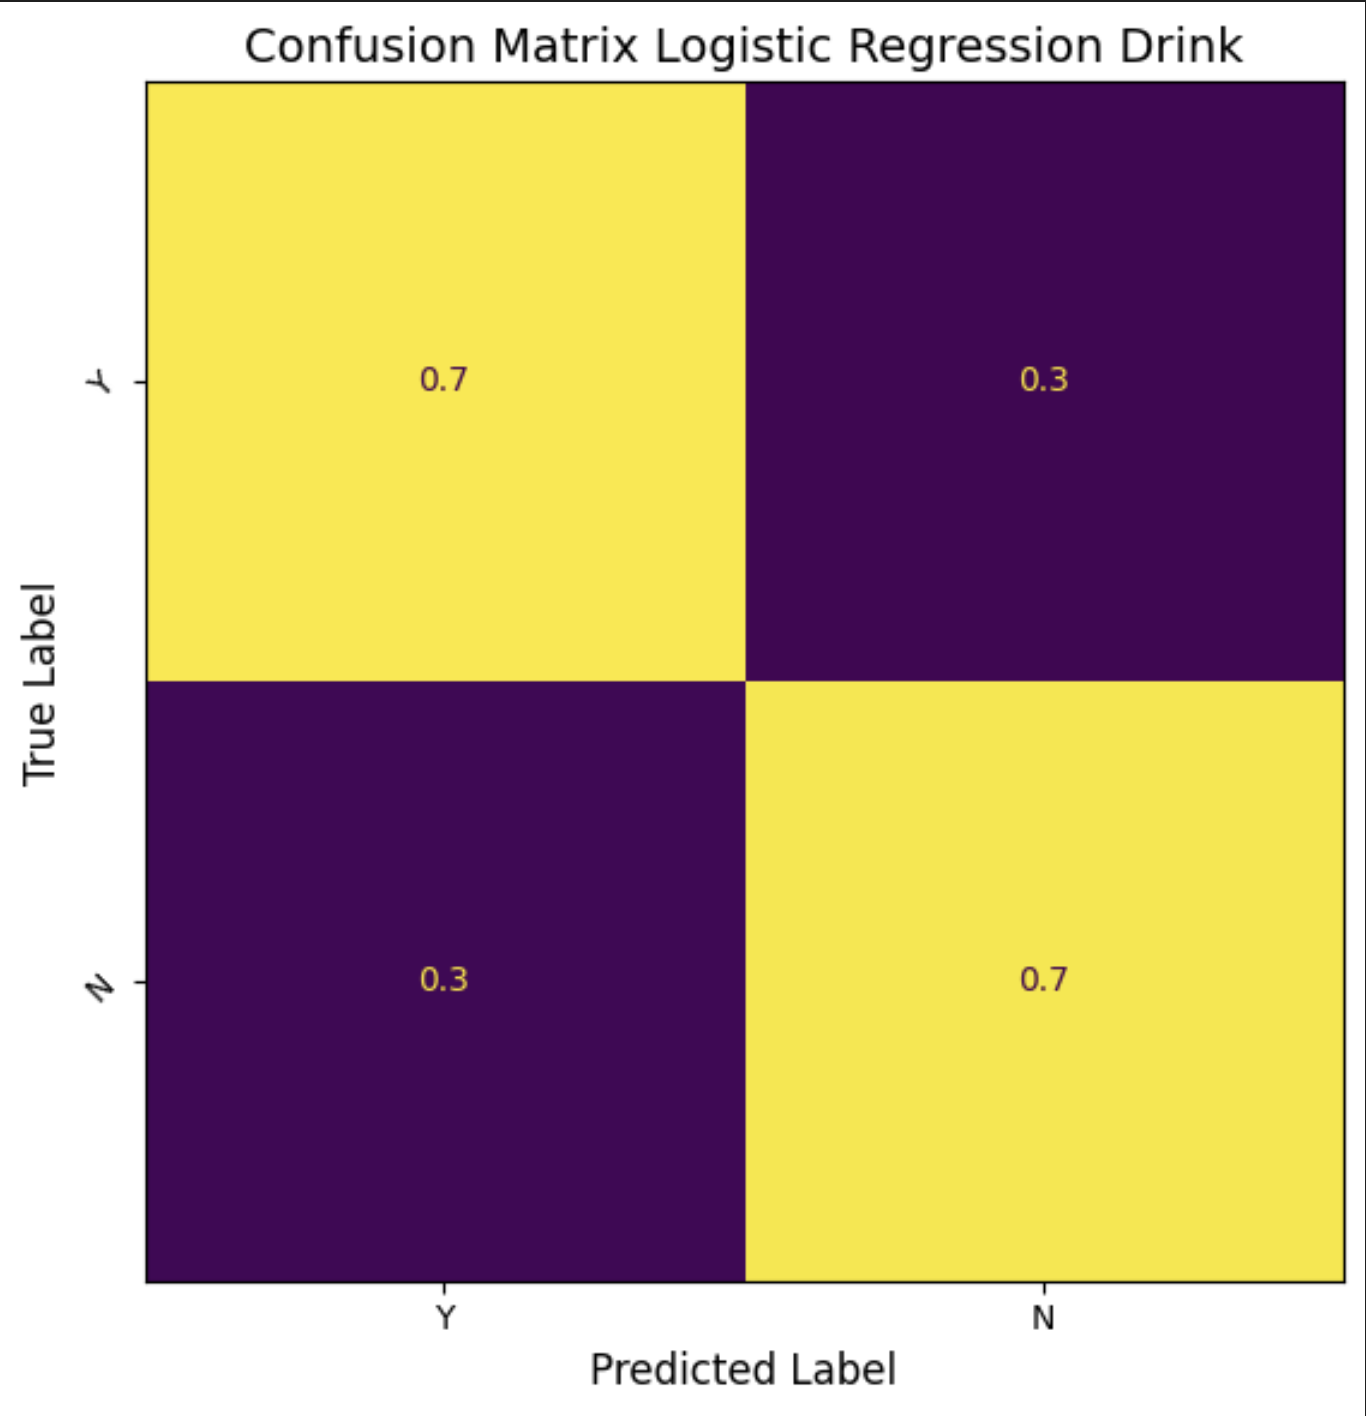
\includegraphics[width=\columnwidth,height=0.75\columnwidth,keepaspectratio]{screen_results/confusion_matrix_first_example_d.png}
\end{minipage}
\end{center}

%%%%%%%%%%%%%%%%%%%%%%%%%%%%%%%%%%%%%%%%%%%%%%%%%%%%%%%%%%%%%%%%%%%%%%%%%%%%%%
% Random Forest
%%%%%%%%%%%%%%%%%%%%%%%%%%%%%%%%%%%%%%%%%%%%%%%%%%%%%%%%%%%%%%%%%%%%%%%%%%%%%%

\subsection{Random Forest}

Di seguito verranno invece riportati i risultati per quanto riguarda quello che abbiamo categorizzato come il miglior modello tra tutti quelli testati: la Random Forest; come si potrà evincere infatti, oltre ad avere la F1-score e l'accuratezza tra le più alte tra tutti i modelli testati, è anche il modello che riesce meglio a separare la classe dei "Non fumatori" dalla classe combinata "Fumatori e Ex-fumatori" e a sua volta è anche la migliore che riesce a separare queste ultime due (anche se comunque non in maniera ottimale).
Per di più, proprio grazie a questi risultati ottenuti dalla Random Forest abbiamo avuto l'idea di testare un classificatore di tipo gerarchico, dunque si è rivelato un modello fondamentale per il nostro progetto.

\paragraph{Cross validation}
Siccome la Random Forest si è rivelato il modello migliore in assoluto, abbiamo anche pensato di fare cross-validation per valutare in maniera più precisa le performance del modello; siccome nello step della feature selection abbiamo allenato il nostro modello tenendo però costante il set di train e di validazione, potremmo aver "overfittato" in base alla suddivisione specifica, quindi con la cross-validation, abbiamo testato il modello su diverse porzioni del dataset per poter valutare in maniera esaustiva il modello. Specifichiamo che avremmo potuto effettuare la cross-validation anche per tutti gli altri modelli, ma vista la quantità di modelli testati ed il tempo necessario per compiere cross-validation ci siamo limitati a farla solo per il modello migliore tra tutti quelli testati.

\subsection*{Smoke (Modello Base)}
\begin{center}
\begin{minipage}[c]{0.50\columnwidth}
\resizebox{\columnwidth}{!}{%
\begin{tabular}{lcccc}
\toprule
Label        & Precision & Recall & F1-score & Support \\
\midrule
Non-smoker   & 0.82      & 0.84   & 0.83     & 167528 \\
Ex-smoker    & 0.44      & 0.35   & 0.39     & 47377  \\
Smoker       & 0.51      & 0.56   & 0.54     & 58574  \\
\midrule
Accuracy     & --        & --     & 0.69     & 273479 \\
Macro avg    & 0.59      & 0.58   & 0.58     & 273479 \\
Weighted avg & 0.69      & 0.69   & 0.69     & 273479 \\
\bottomrule
\end{tabular}%
}
\end{minipage}\hspace{\columnsep}%
\begin{minipage}[c]{0.40\columnwidth}
\centering
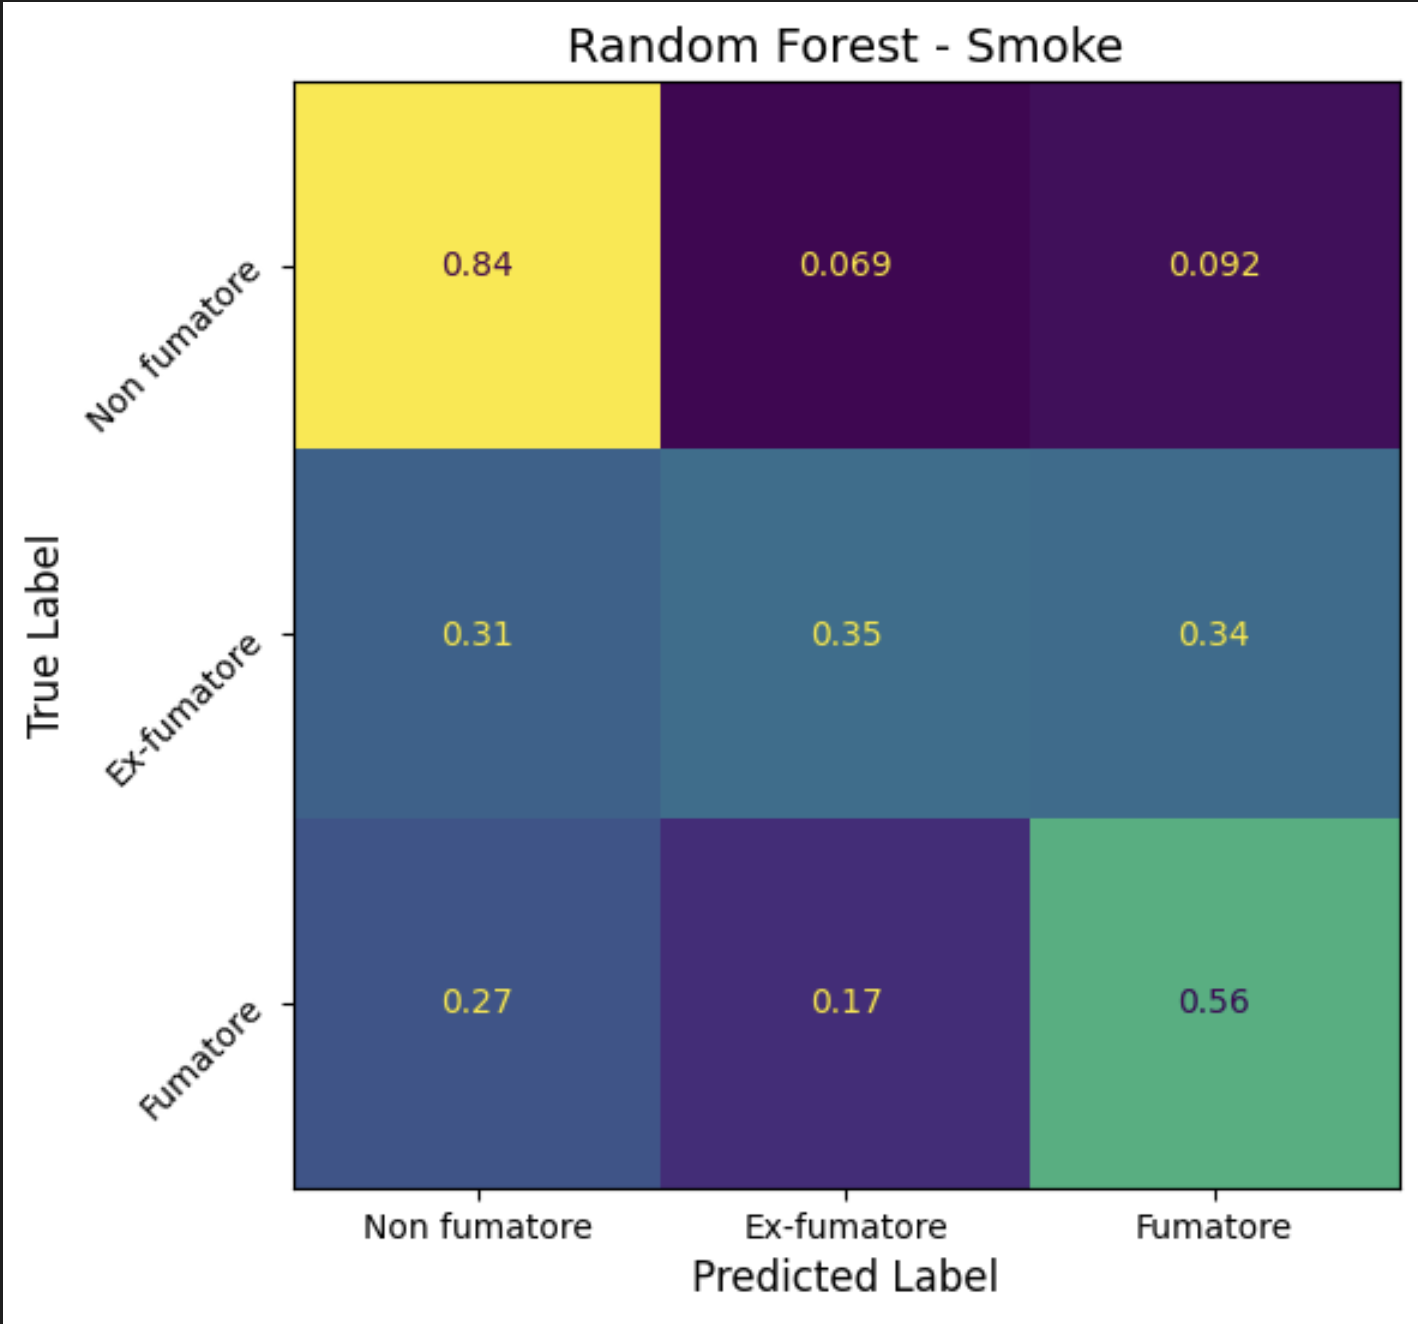
\includegraphics[width=\columnwidth,height=0.75\columnwidth,keepaspectratio]{screen_results/confusion_matrix_rf_base_s.png}
\end{minipage}
\end{center}

\subsection*{Drink (Modello Base)}
\begin{center}
\begin{minipage}[c]{0.50\columnwidth}
\resizebox{\columnwidth}{!}{%
\begin{tabular}{lcccc}
\toprule
Label  & Precision & Recall & F1-score & Support \\
\midrule
Y      & 0.72      & 0.71   & 0.72     & 135539 \\
N      & 0.72      & 0.73   & 0.73     & 137940 \\
\midrule
Accuracy     & --        & --     & 0.72     & 273479 \\
Macro avg    & 0.72      & 0.72   & 0.72     & 273479 \\
Weighted avg & 0.72      & 0.72   & 0.72     & 273479 \\
\bottomrule
\end{tabular}%
}
\end{minipage}\hspace{\columnsep}%
\begin{minipage}[c]{0.40\columnwidth}
\centering
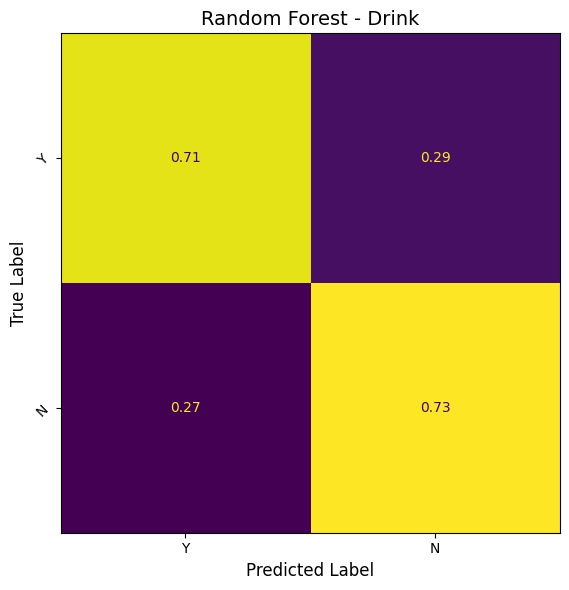
\includegraphics[width=\columnwidth,height=0.75\columnwidth,keepaspectratio]{screen_results/confusion_matrix_rf_base_d.png}
\end{minipage}
\end{center}

\label{bestmodel_smoke}
\subsection*{Smoke (Modello Ottimizzato)}
\begin{center}
\begin{minipage}[c]{0.50\columnwidth}
\resizebox{\columnwidth}{!}{%
\begin{tabular}{lcccc}
\toprule
Label        & Precision & Recall & F1-score & Support \\
\midrule
Non-smoker   & 0.94      & 0.73   & 0.82     & 179990 \\
Ex-smoker    & 0.41      & 0.58   & 0.48     & 52103  \\
Smoker       & 0.49      & 0.64   & 0.55     & 63429  \\
\midrule
Accuracy     & --        & --     & 0.68     & 295522 \\
Macro avg    & 0.61      & 0.65   & 0.62     & 295522 \\
Weighted avg & 0.75      & 0.68   & 0.70     & 295522 \\
\bottomrule
\end{tabular}%
}
\end{minipage}\hspace{\columnsep}%
\begin{minipage}[c]{0.40\columnwidth}
\centering
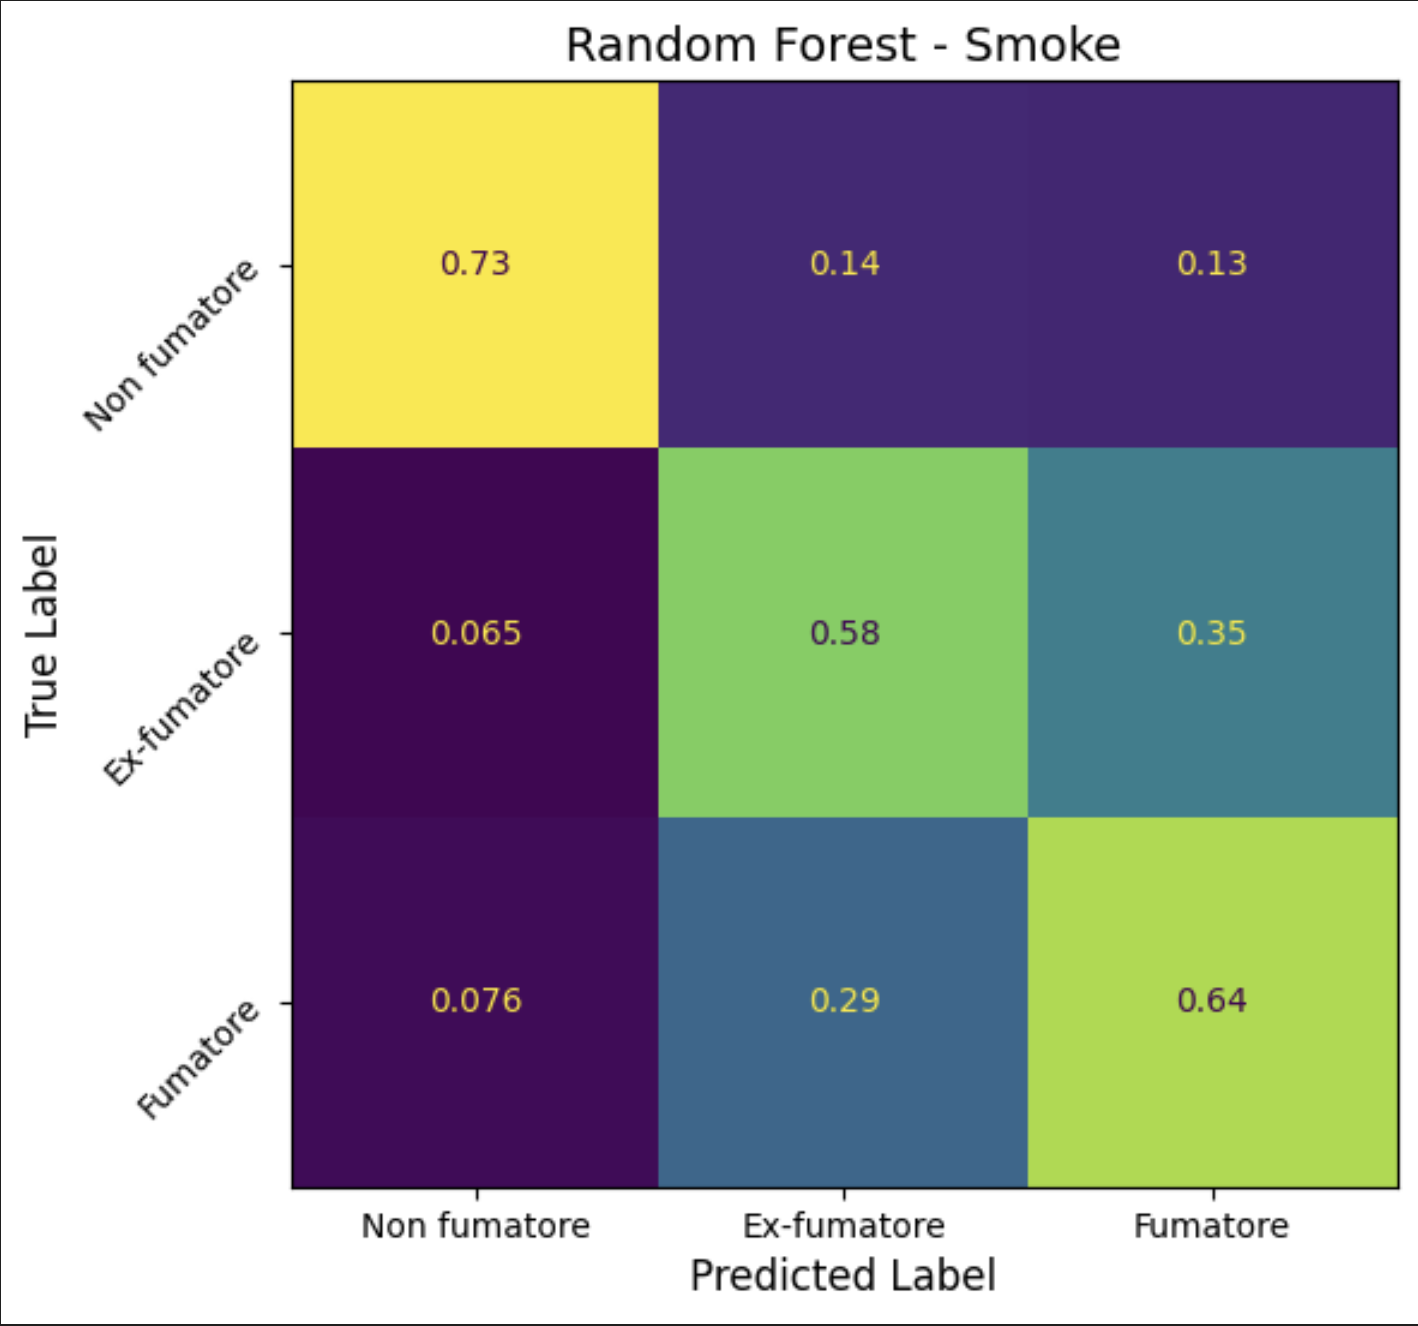
\includegraphics[width=\columnwidth,height=0.75\columnwidth,keepaspectratio]{screen_results/confusion_matrix_rf_optimized_s.png}
\end{minipage}
\end{center}

\label{bestmodel_drink}
\subsection*{Drink (Modello Ottimizzato)}
\begin{center}
\begin{minipage}[c]{0.50\columnwidth}
\resizebox{\columnwidth}{!}{%
\begin{tabular}{lcccc}
\toprule
Label  & Precision & Recall & F1-score & Support \\
\midrule
Y      & 0.74      & 0.71   & 0.73     & 147869 \\
N      & 0.72      & 0.75   & 0.74     & 147653 \\
\midrule
Accuracy     & --        & --     & 0.73     & 295522 \\
Macro avg    & 0.73      & 0.73   & 0.73     & 295522 \\
Weighted avg & 0.73      & 0.73   & 0.73     & 295522 \\
\bottomrule
\end{tabular}%
}
\end{minipage}\hspace{\columnsep}%
\begin{minipage}[c]{0.40\columnwidth}
\centering
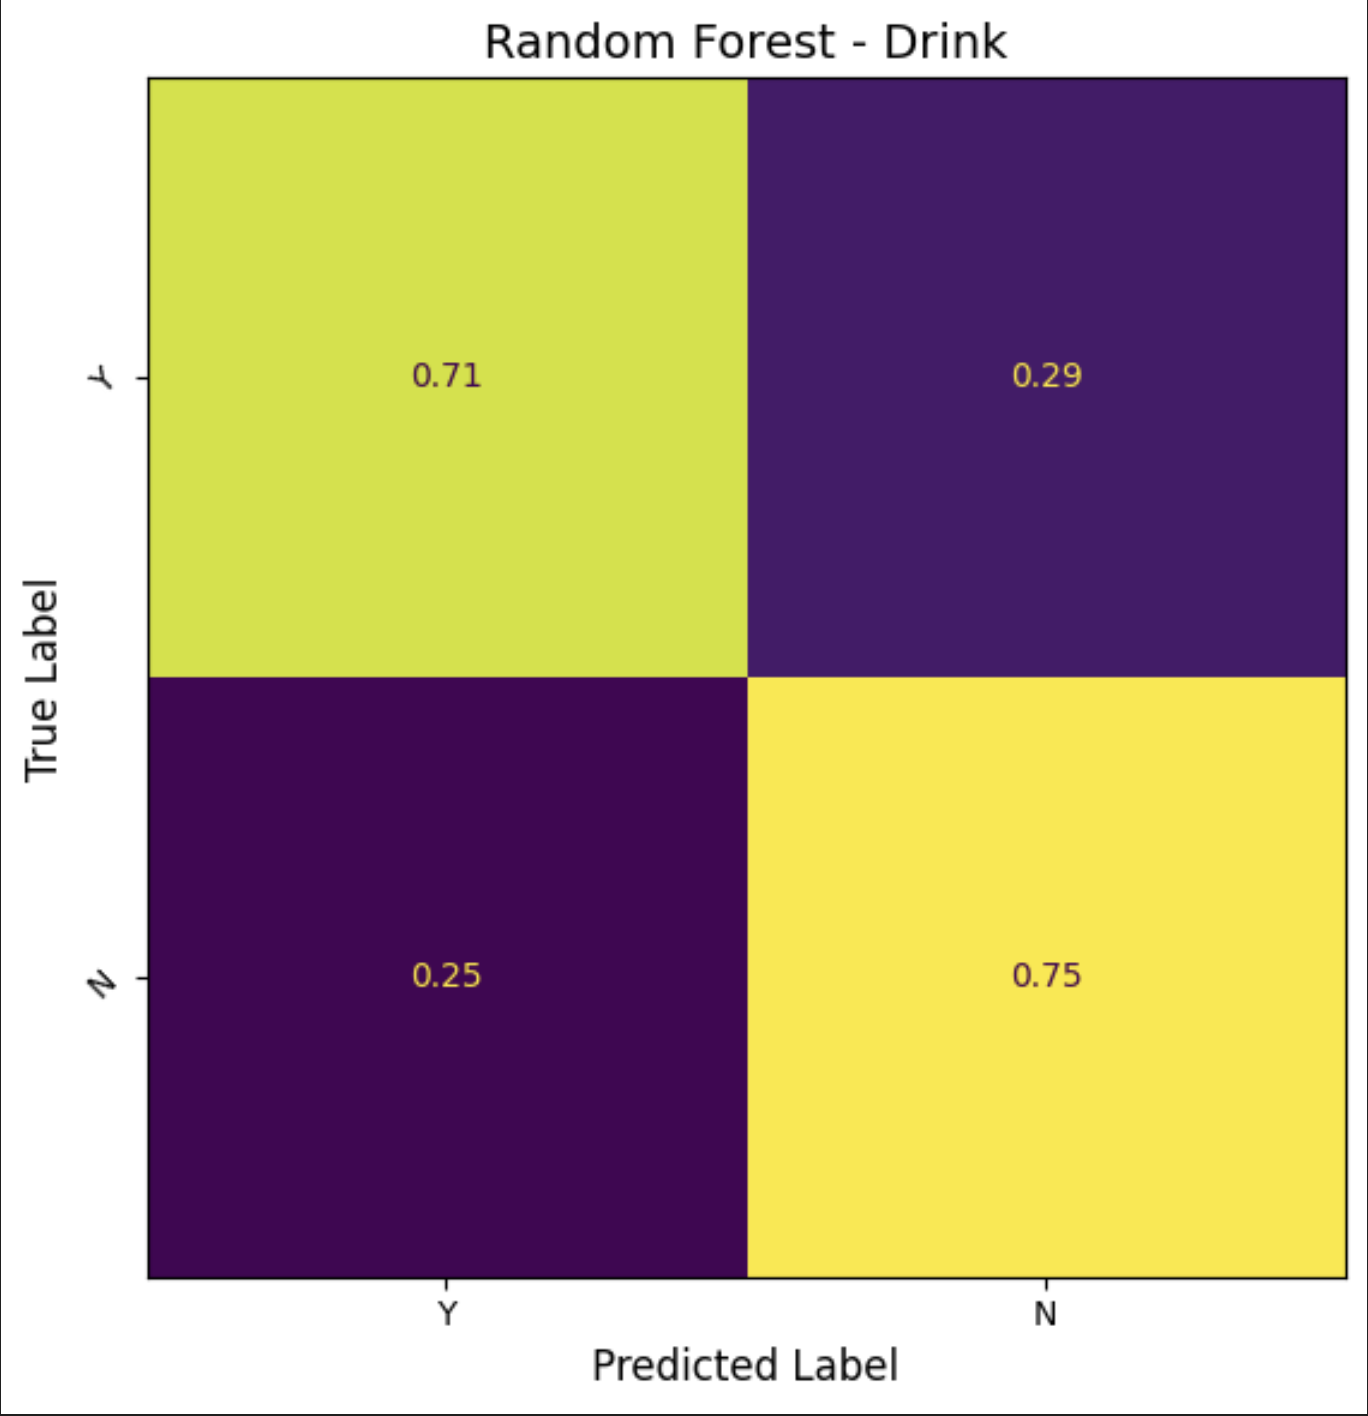
\includegraphics[width=\columnwidth,height=0.75\columnwidth,keepaspectratio]{screen_results/confusion_matrix_rf_optimized_d.png}
\end{minipage}
\end{center}

%%%%%%%%%%%%%%%%%%%%%%%%%%%%%%%%%%%%%%%%%%%%%%%%%%%%%%%%%%%%%%%%%%%%%%%%%%%%%%
% Altri modelli (SVM lineare, KNN, AdaBoost)
%%%%%%%%%%%%%%%%%%%%%%%%%%%%%%%%%%%%%%%%%%%%%%%%%%%%%%%%%%%%%%%%%%%%%%%%%%%%%%

\subsection{Altri modelli (SVM lineare, KNN, AdaBoost)}

Per poter confrontare i risultati della Random Forest con tutti gli altri modelli testati, riportiamo anche i risultati di questi appena citati; come si potrà evincere, qualche modello (come SVM) si avvicina molto alle performance della Random Forest ma risulta comunque leggermente peggiore, mentre per altri modelli si noterà marcatamente la differenza non tanto di metriche come la F1-score quanto della capacità di classificare i sample appartenenti agli "Ex-fumatori" e "Fumatori".
Purtroppo per quanto riguarda la classificazione riguardante il consumo di alcool, da adesso in poi rimarrà praticamente la medesima.

\subsection*{AdaBoost (Smoke)}
\begin{center}
\begin{minipage}[c]{0.50\columnwidth}
\resizebox{\columnwidth}{!}{%
\begin{tabular}{lcccc}
\toprule
Label        & Precision & Recall & F1-score & Support \\
\midrule
Non-smoker   & 0.83      & 0.83   & 0.83     & 119747 \\
Ex-smoker    & 0.45      & 0.32   & 0.37     & 34738  \\
Smoker       & 0.50      & 0.63   & 0.56     & 42530  \\
\midrule
Accuracy     & --        & --     & 0.70     & 197015 \\
Macro avg    & 0.59      & 0.59   & 0.59     & 197015 \\
Weighted avg & 0.69      & 0.70   & 0.69     & 197015 \\
\bottomrule
\end{tabular}%
}
\end{minipage}\hspace{\columnsep}%
\begin{minipage}[c]{0.40\columnwidth}
\centering
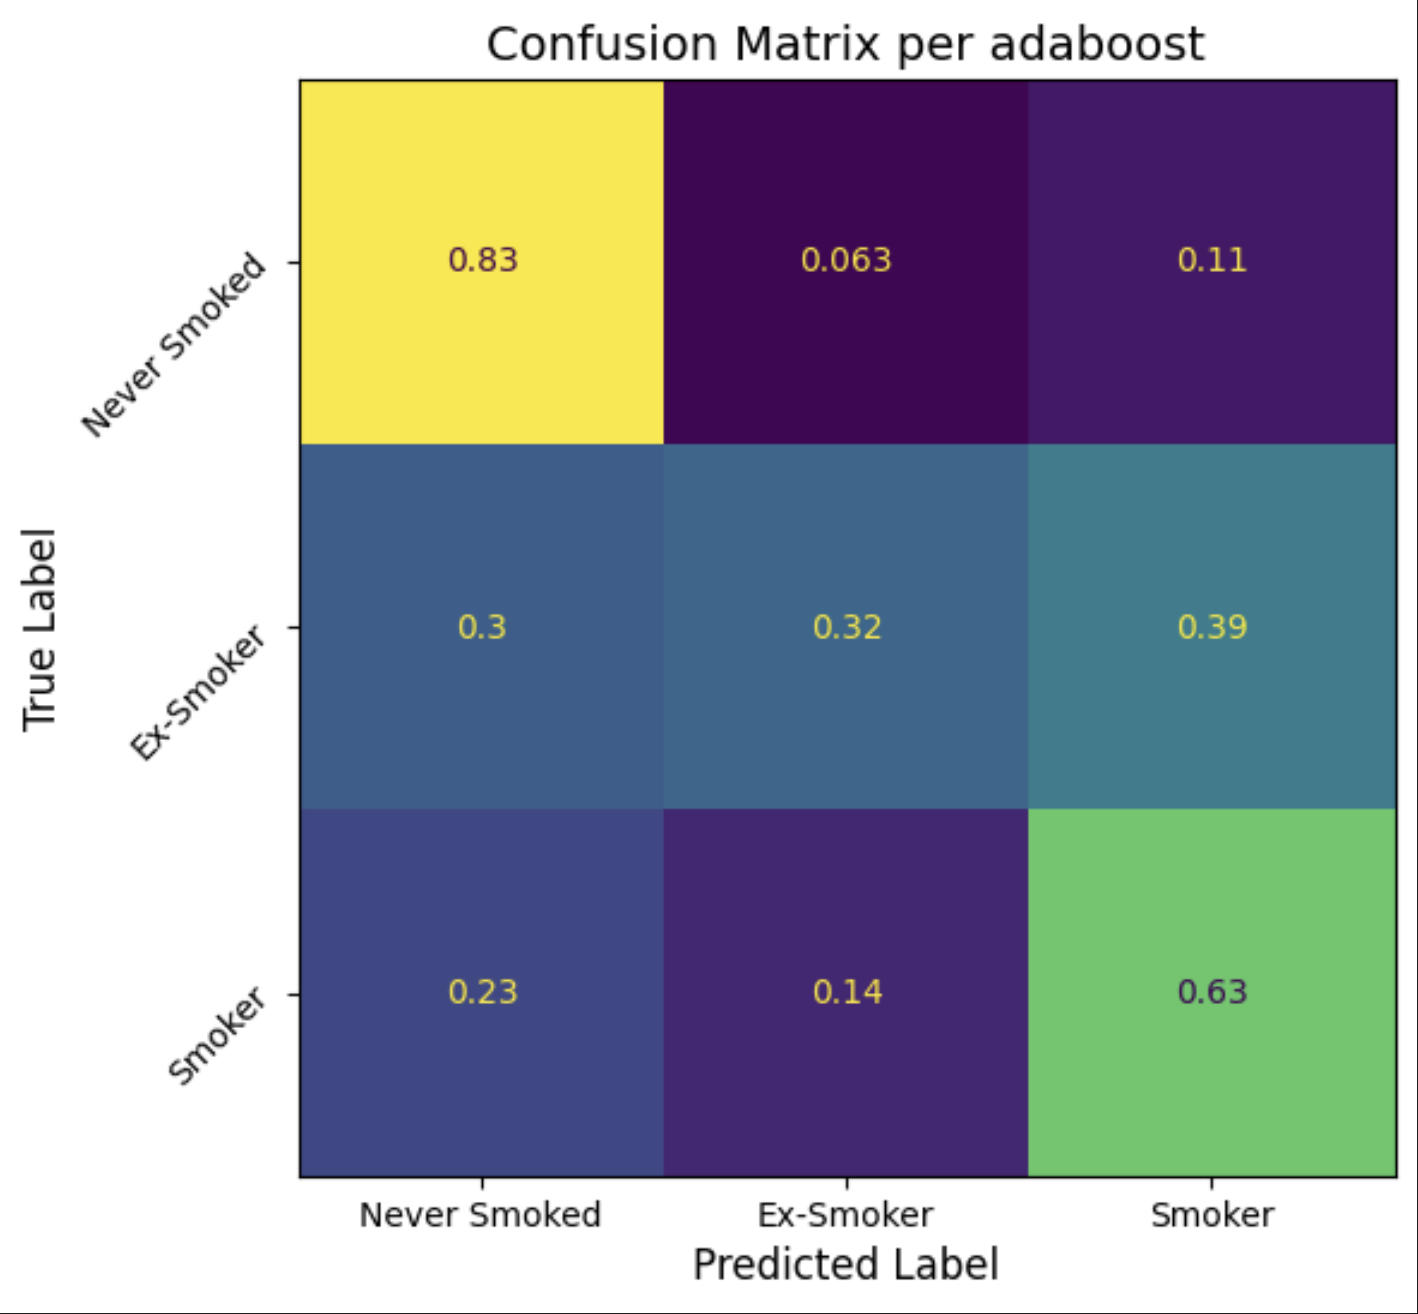
\includegraphics[width=\columnwidth,height=0.75\columnwidth,keepaspectratio]{screen_results/confusion_matrix_adaboost_s.png}
\end{minipage}
\end{center}

\subsection*{SVM (Smoke)}
\begin{center}
\begin{minipage}[c]{0.50\columnwidth}
\resizebox{\columnwidth}{!}{%
\begin{tabular}{lcccc}
\toprule
Label        & Precision & Recall & F1-score & Support \\
\midrule
Non-smoker   & 0.94      & 0.73   & 0.82     & 119747 \\
Ex-smoker    & 0.41      & 0.55   & 0.47     & 34738  \\
Smoker       & 0.47      & 0.65   & 0.55     & 42530  \\
\midrule
Accuracy     & --        & --     & 0.68     & 197015 \\
Macro avg    & 0.61      & 0.64   & 0.61     & 197015 \\
Weighted avg & 0.75      & 0.68   & 0.70     & 197015 \\
\bottomrule
\end{tabular}%
}
\end{minipage}\hspace{\columnsep}%
\begin{minipage}[c]{0.40\columnwidth}
\centering
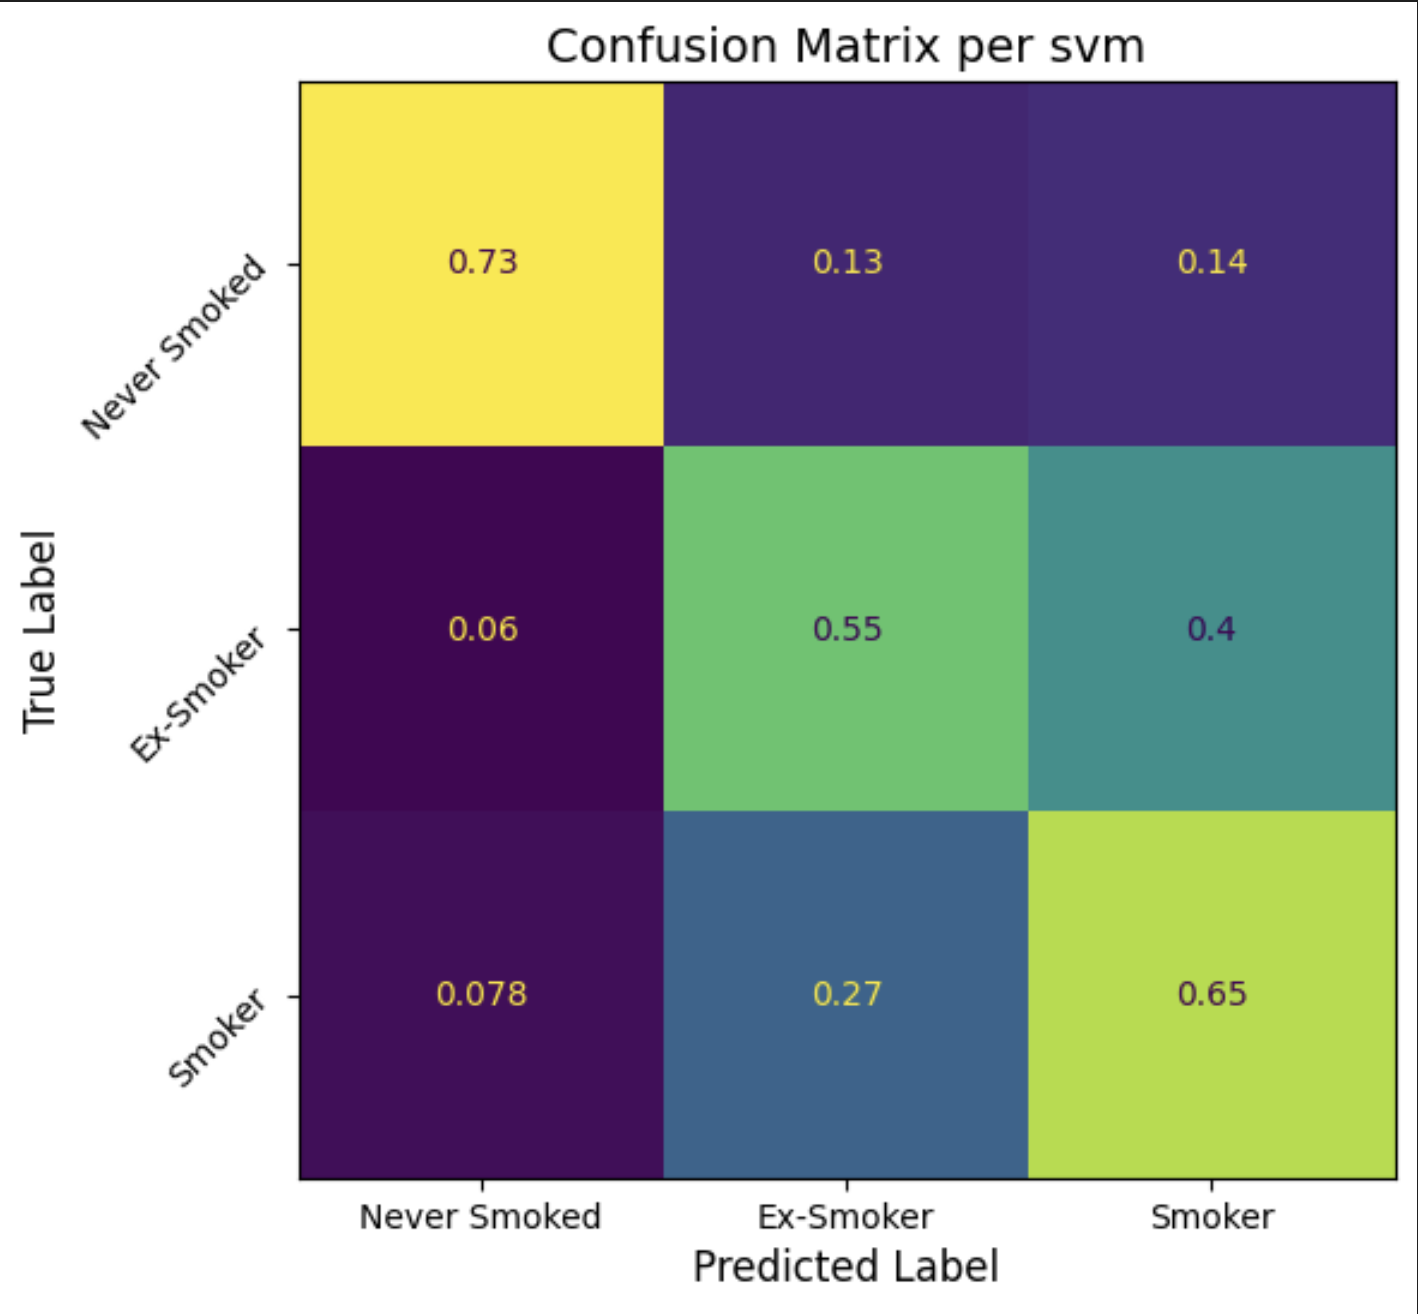
\includegraphics[width=\columnwidth,height=0.75\columnwidth,keepaspectratio]{screen_results/confusion_matrix_svm_s.png}
\end{minipage}
\end{center}

\subsection*{KNN (Smoke)}
\begin{center}
\begin{minipage}[c]{0.50\columnwidth}
\resizebox{\columnwidth}{!}{%
\begin{tabular}{lcccc}
\toprule
Label        & Precision & Recall & F1-score & Support \\
\midrule
Non-smoker   & 0.85      & 0.80   & 0.83     & 119747 \\
Ex-smoker    & 0.44      & 0.43   & 0.43     & 34738  \\
Smoker       & 0.49      & 0.59   & 0.54     & 42530  \\
\midrule
Accuracy     & --        & --     & 0.69     & 197015 \\
Macro avg    & 0.60      & 0.61   & 0.60     & 197015 \\
Weighted avg & 0.70      & 0.69   & 0.70     & 197015 \\
\bottomrule
\end{tabular}%
}
\end{minipage}\hspace{\columnsep}%
\begin{minipage}[c]{0.40\columnwidth}
\centering
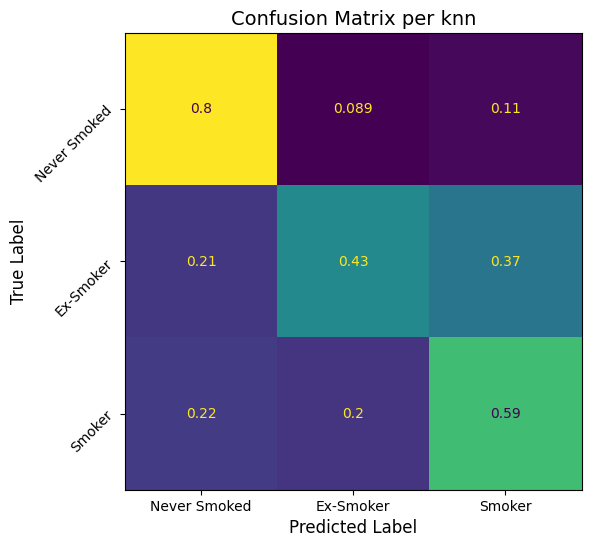
\includegraphics[width=\columnwidth,height=0.75\columnwidth,keepaspectratio]{screen_results/confusion_matrix_knn_s.png}
\end{minipage}
\end{center}

\subsection*{AdaBoost (Drink)}
\begin{center}
\begin{minipage}[c]{0.50\columnwidth}
\resizebox{\columnwidth}{!}{%
\begin{tabular}{lcccc}
\toprule
Label & Precision & Recall & F1-score & Support \\
\midrule
Y     & 0.73      & 0.73   & 0.73     & 98396 \\
N     & 0.73      & 0.73   & 0.73     & 98619 \\
\midrule
Accuracy     & --        & --     & 0.73     & 197015 \\
Macro avg    & 0.73      & 0.73   & 0.73     & 197015 \\
Weighted avg & 0.73      & 0.73   & 0.73     & 197015 \\
\bottomrule
\end{tabular}%
}
\end{minipage}\hspace{\columnsep}%
\begin{minipage}[c]{0.40\columnwidth}
\centering
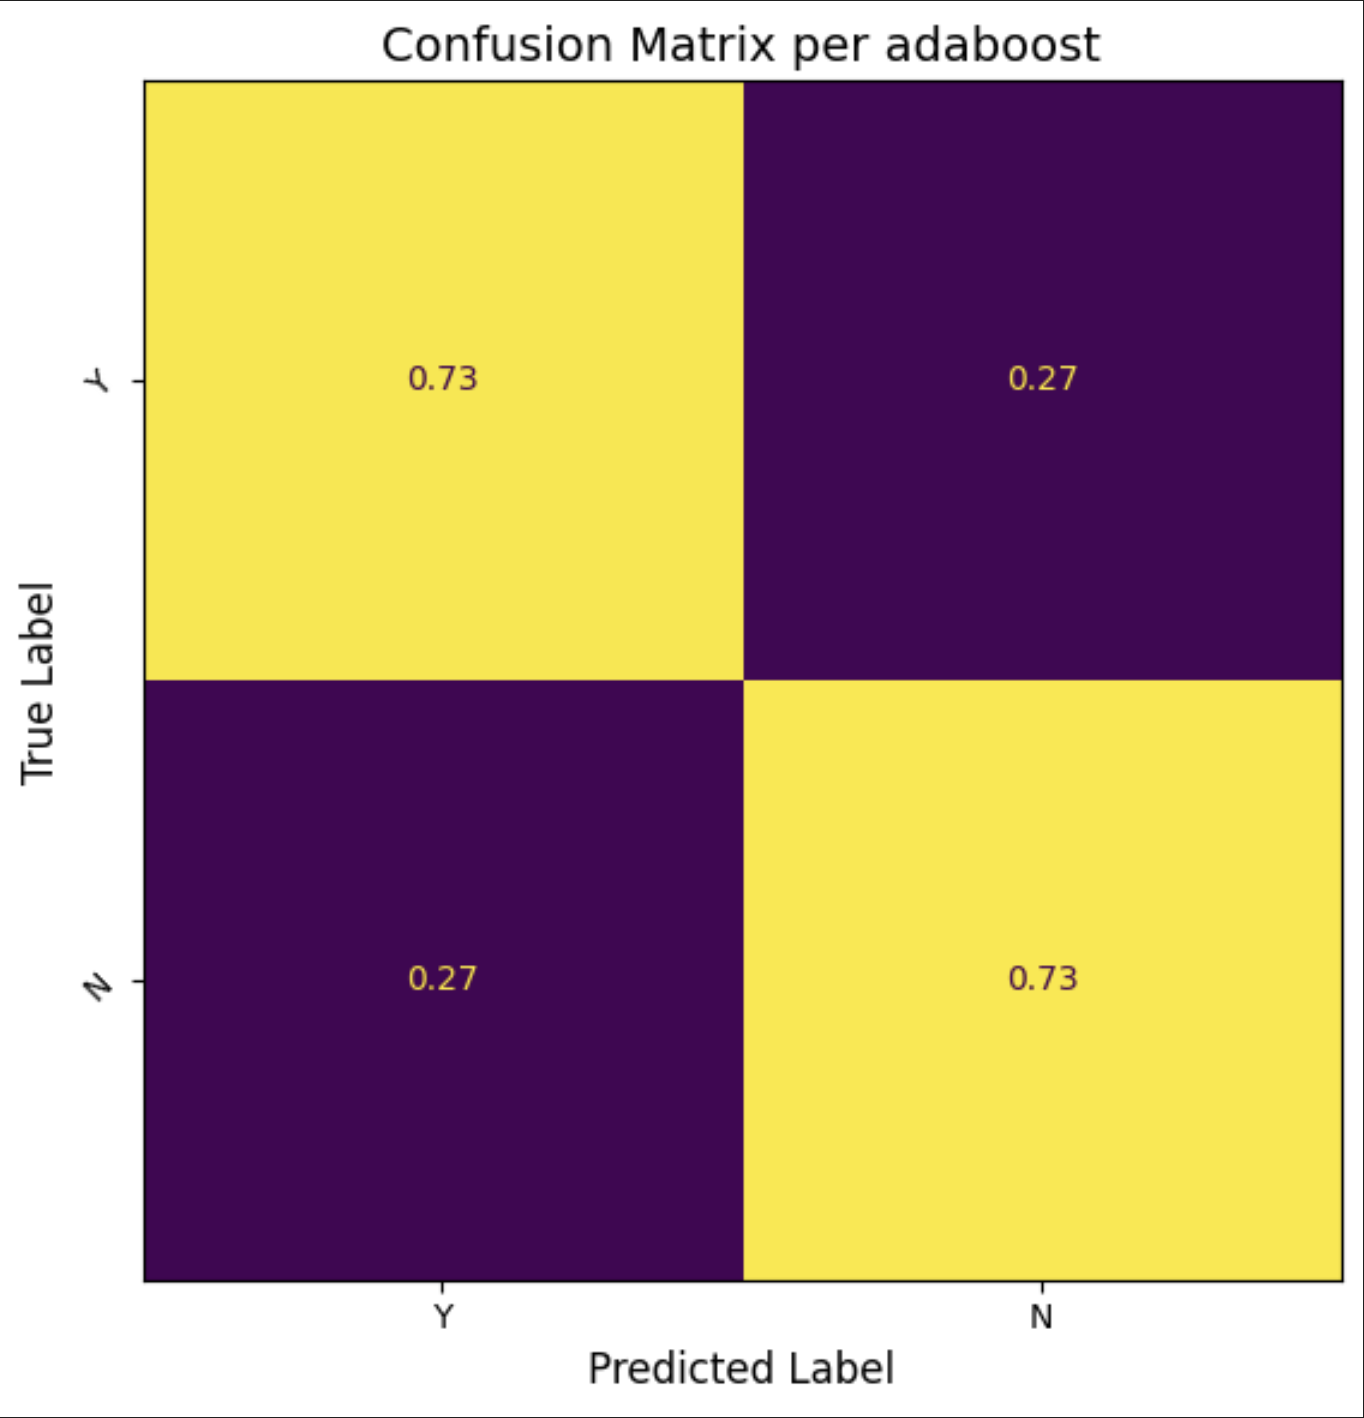
\includegraphics[width=\columnwidth,height=0.75\columnwidth,keepaspectratio]{screen_results/confusion_matrix_adaboost_d.png}
\end{minipage}
\end{center}

\subsection*{SVM (Drink)}
\begin{center}
\begin{minipage}[c]{0.50\columnwidth}
\resizebox{\columnwidth}{!}{%
\begin{tabular}{lcccc}
\toprule
Label & Precision & Recall & F1-score & Support \\
\midrule
Y     & 0.72      & 0.72   & 0.72     & 98396 \\
N     & 0.72      & 0.72   & 0.72     & 98619 \\
\midrule
Accuracy     & --        & --     & 0.72     & 197015 \\
Macro avg    & 0.72      & 0.72   & 0.72     & 197015 \\
Weighted avg & 0.72      & 0.72   & 0.72     & 197015 \\
\bottomrule
\end{tabular}%
}
\end{minipage}\hspace{\columnsep}%
\begin{minipage}[c]{0.40\columnwidth}
\centering
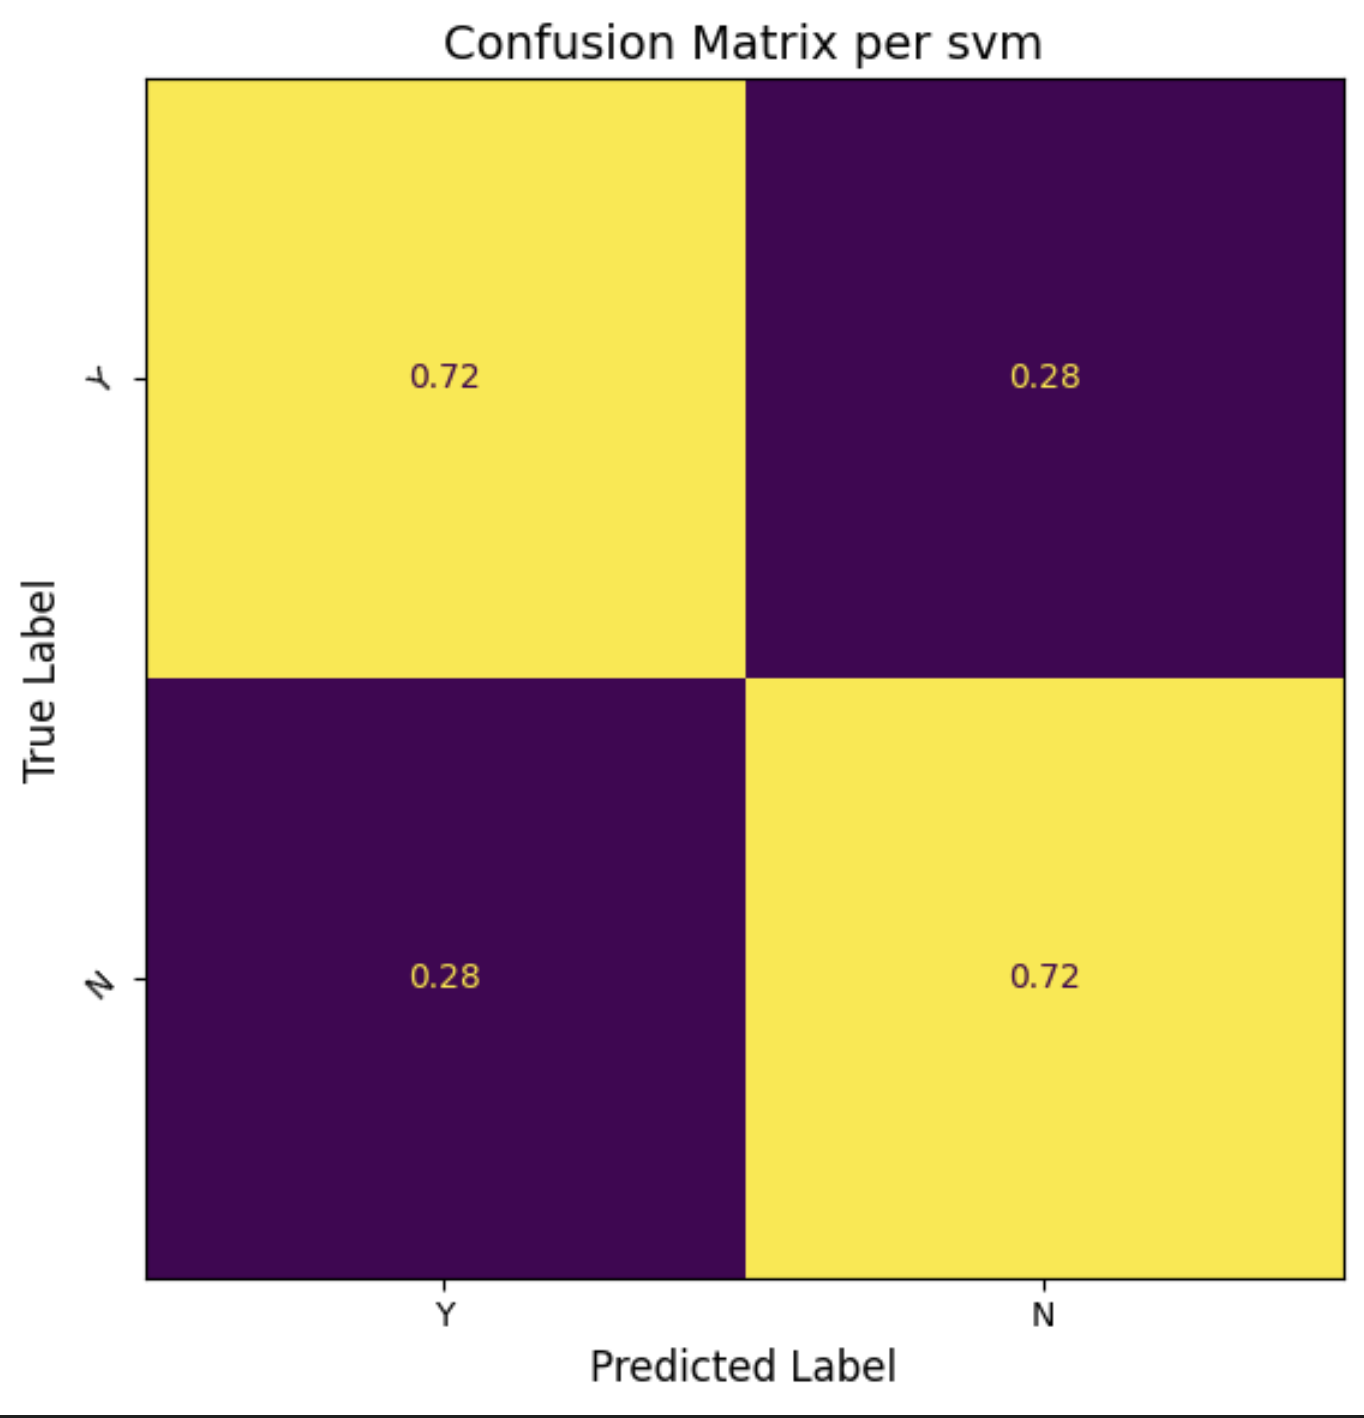
\includegraphics[width=\columnwidth,height=0.75\columnwidth,keepaspectratio]{screen_results/confusion_matrix_svm_d.png}
\end{minipage}
\end{center}

\subsection*{KNN (Drink)}
\begin{center}
\begin{minipage}[c]{0.50\columnwidth}
\resizebox{\columnwidth}{!}{%
\begin{tabular}{lcccc}
\toprule
Label & Precision & Recall & F1-score & Support \\
\midrule
Y     & 0.73      & 0.67   & 0.70     & 98396 \\
N     & 0.70      & 0.76   & 0.73     & 98619 \\
\midrule
Accuracy     & --        & --     & 0.71     & 197015 \\
Macro avg    & 0.72      & 0.71   & 0.71     & 197015 \\
Weighted avg & 0.72      & 0.71   & 0.71     & 197015 \\
\bottomrule
\end{tabular}%
}
\end{minipage}\hspace{\columnsep}%
\begin{minipage}[c]{0.40\columnwidth}
\centering
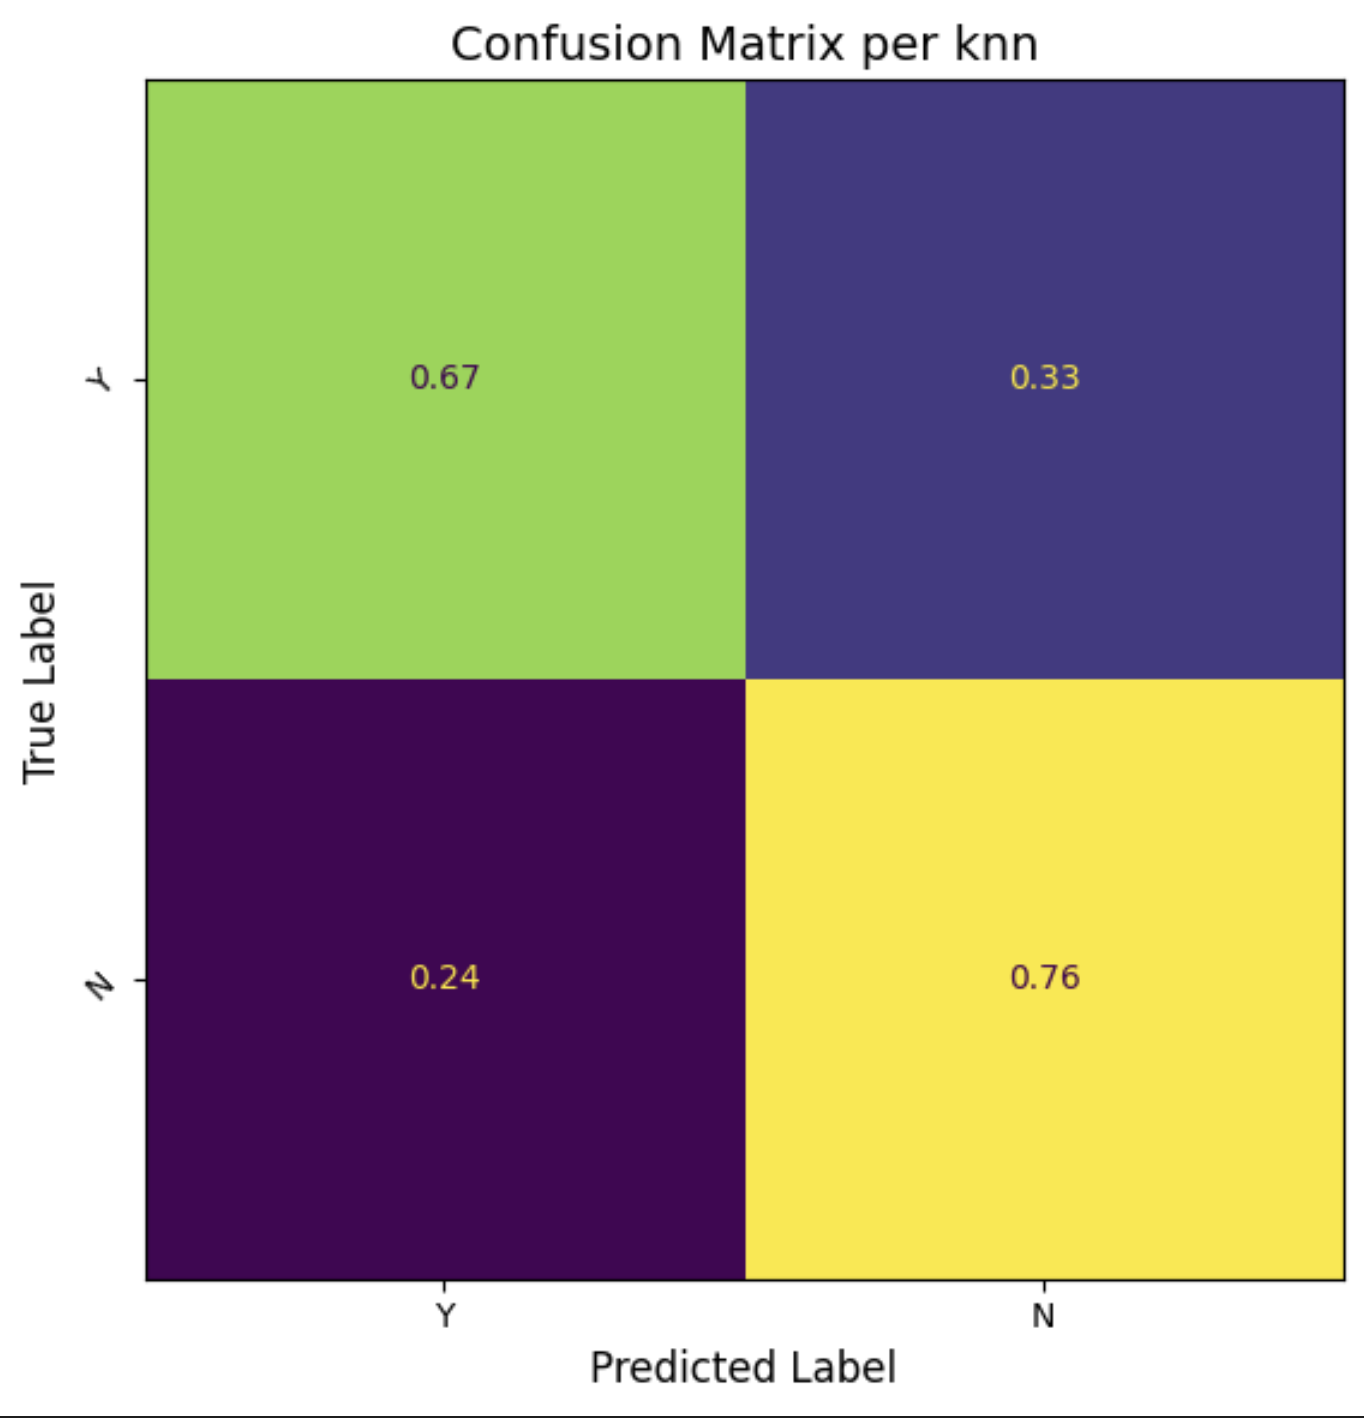
\includegraphics[width=\columnwidth,height=0.75\columnwidth,keepaspectratio]{screen_results/confusion_matrix_knn_d.png}
\end{minipage}
\end{center}

%%%%%%%%%%%%%%%%%%%%%%%%%%%%%%%%%%%%%%%%%%%%%%%%%%%%%%%%%%%%%%%%%%%%%%%%%%%%%%
% Altri modelli con PCA (SVM, KNN)
%%%%%%%%%%%%%%%%%%%%%%%%%%%%%%%%%%%%%%%%%%%%%%%%%%%%%%%%%%%%%%%%%%%%%%%%%%%%%%

\subsection{Altri modelli con PCA (SVM, KNN)}
Come già accennato nella sezione precedente, abbiamo anche testato l'utilizzo della PCA per quanto riguarda i modelli KNN e SVM; purtroppo i risultati non hanno portato a dei miglioramenti.

\subsection*{SVM (Smoke) }
\begin{center}
\begin{minipage}[c]{0.50\columnwidth}
\resizebox{\columnwidth}{!}{%
\begin{tabular}{lcccc}
\toprule
Label        & Precision & Recall & F1-score & Support \\
\midrule
Non-smoker   & 0.89      & 0.76   & 0.82     & 120489 \\
Ex-smoker    & 0.41      & 0.44   & 0.43     & 34990  \\
Smoker       & 0.48      & 0.63   & 0.54     & 42791  \\
\midrule
Accuracy     & --        & --     & 0.68     & 198270 \\
Macro avg    & 0.59      & 0.61   & 0.60     & 198270 \\
Weighted avg & 0.71      & 0.68   & 0.69     & 198270 \\
\bottomrule
\end{tabular}%
}
\end{minipage}\hspace{\columnsep}%
\begin{minipage}[c]{0.40\columnwidth}
\centering
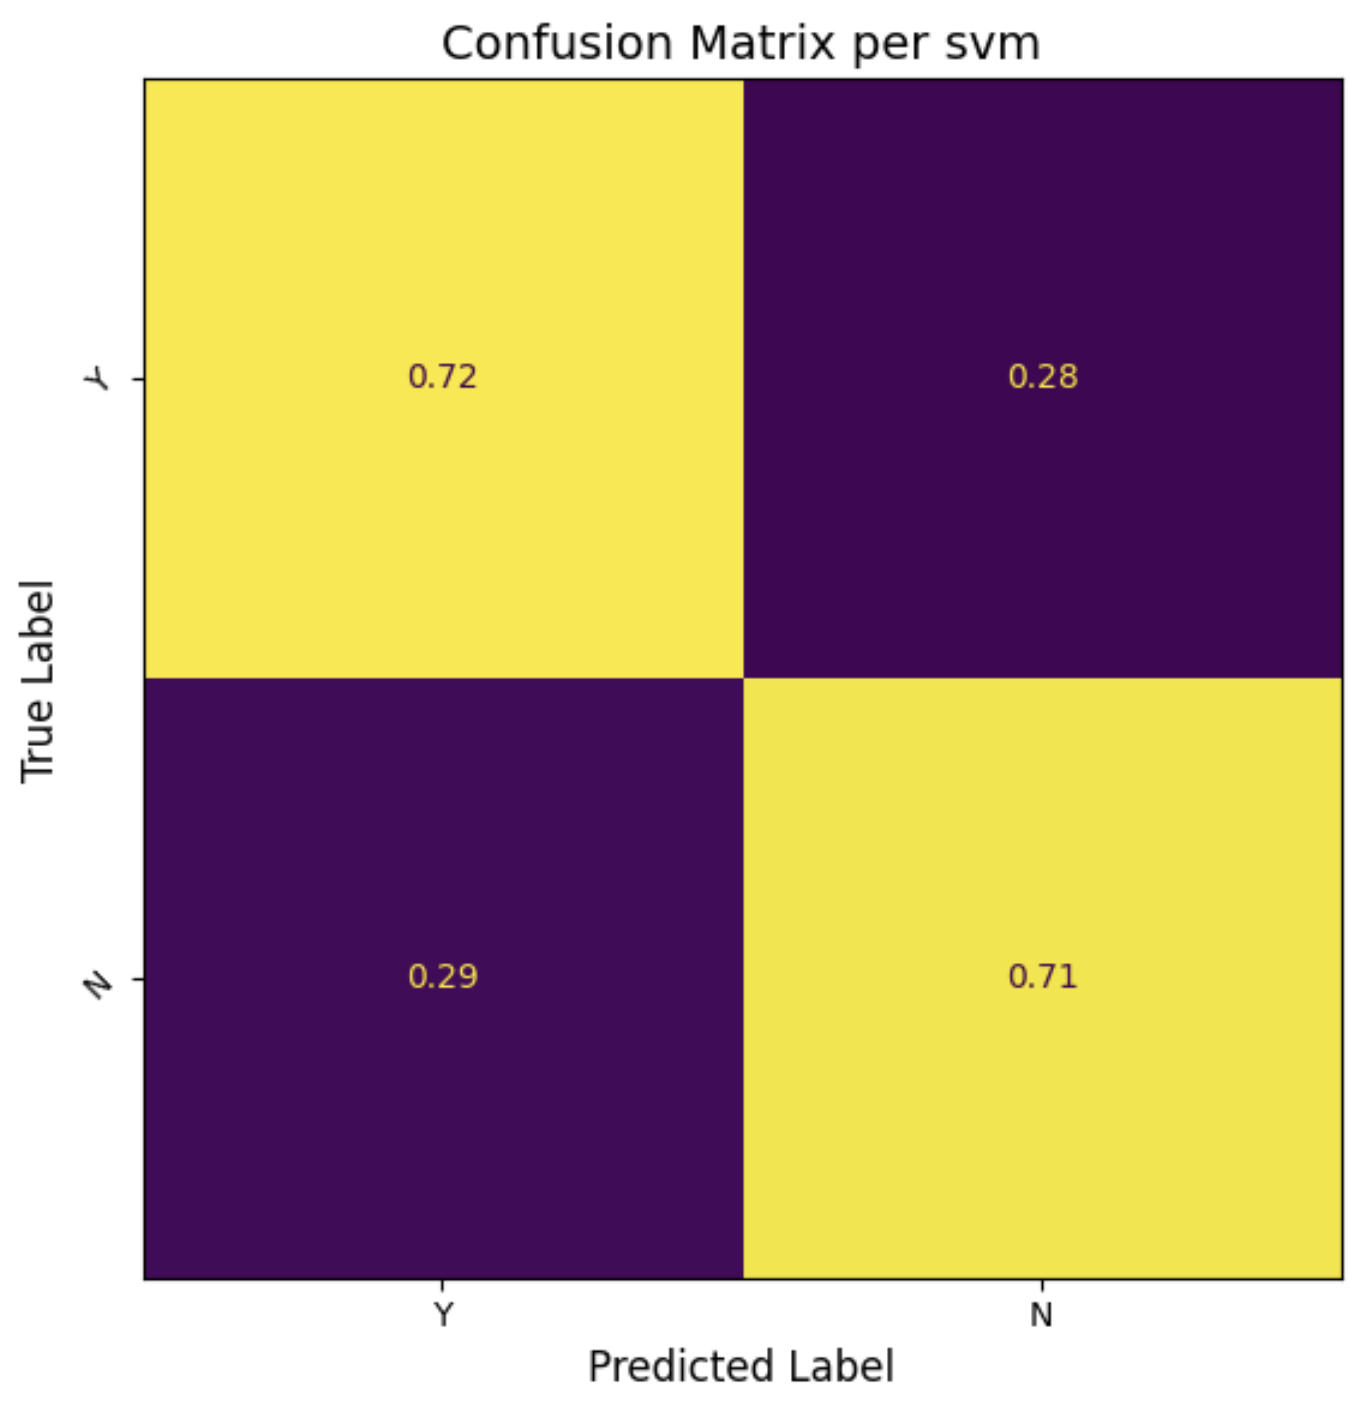
\includegraphics[width=\columnwidth,height=0.75\columnwidth,keepaspectratio]{screen_results/confusion_matrix_svm_pca_d.png} % Adjust image file if needed.
\end{minipage}
\end{center}

\subsection*{KNN (Smoke) }
\begin{center}
\begin{minipage}[c]{0.50\columnwidth}
\resizebox{\columnwidth}{!}{%
\begin{tabular}{lcccc}
\toprule
Label        & Precision & Recall & F1-score & Support \\
\midrule
Non-smoker   & 0.82      & 0.82   & 0.82     & 120489 \\
Ex-smoker    & 0.43      & 0.34   & 0.38     & 34990  \\
Smoker       & 0.49      & 0.57   & 0.53     & 42791  \\
\midrule
Accuracy     & --        & --     & 0.68     & 198270 \\
Macro avg    & 0.58      & 0.58   & 0.58     & 198270 \\
Weighted avg & 0.68      & 0.68   & 0.68     & 198270 \\
\bottomrule
\end{tabular}%
}
\end{minipage}\hspace{\columnsep}%
\begin{minipage}[c]{0.40\columnwidth}
\centering
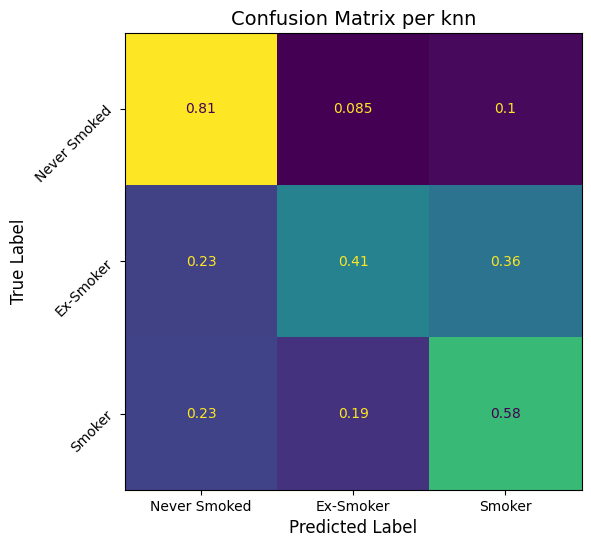
\includegraphics[width=\columnwidth,height=0.75\columnwidth,keepaspectratio]{screen_results/confusion_matrix_knn_pca_s.png}
\end{minipage}
\end{center}

\subsection*{SVM (Drink) }
\begin{center}
\begin{minipage}[c]{0.50\columnwidth}
\resizebox{\columnwidth}{!}{%
\begin{tabular}{lcccc}
\toprule
Label & Precision & Recall & F1-score & Support \\
\midrule
Y     & 0.72      & 0.72   & 0.72     & 99172 \\
N     & 0.72      & 0.72   & 0.72     & 99098 \\
\midrule
Accuracy     & --        & --     & 0.72     & 198270 \\
Macro avg    & 0.72      & 0.72   & 0.72     & 198270 \\
Weighted avg & 0.72      & 0.72   & 0.72     & 198270 \\
\bottomrule
\end{tabular}%
}
\end{minipage}\hspace{\columnsep}%
\begin{minipage}[c]{0.40\columnwidth}
\centering
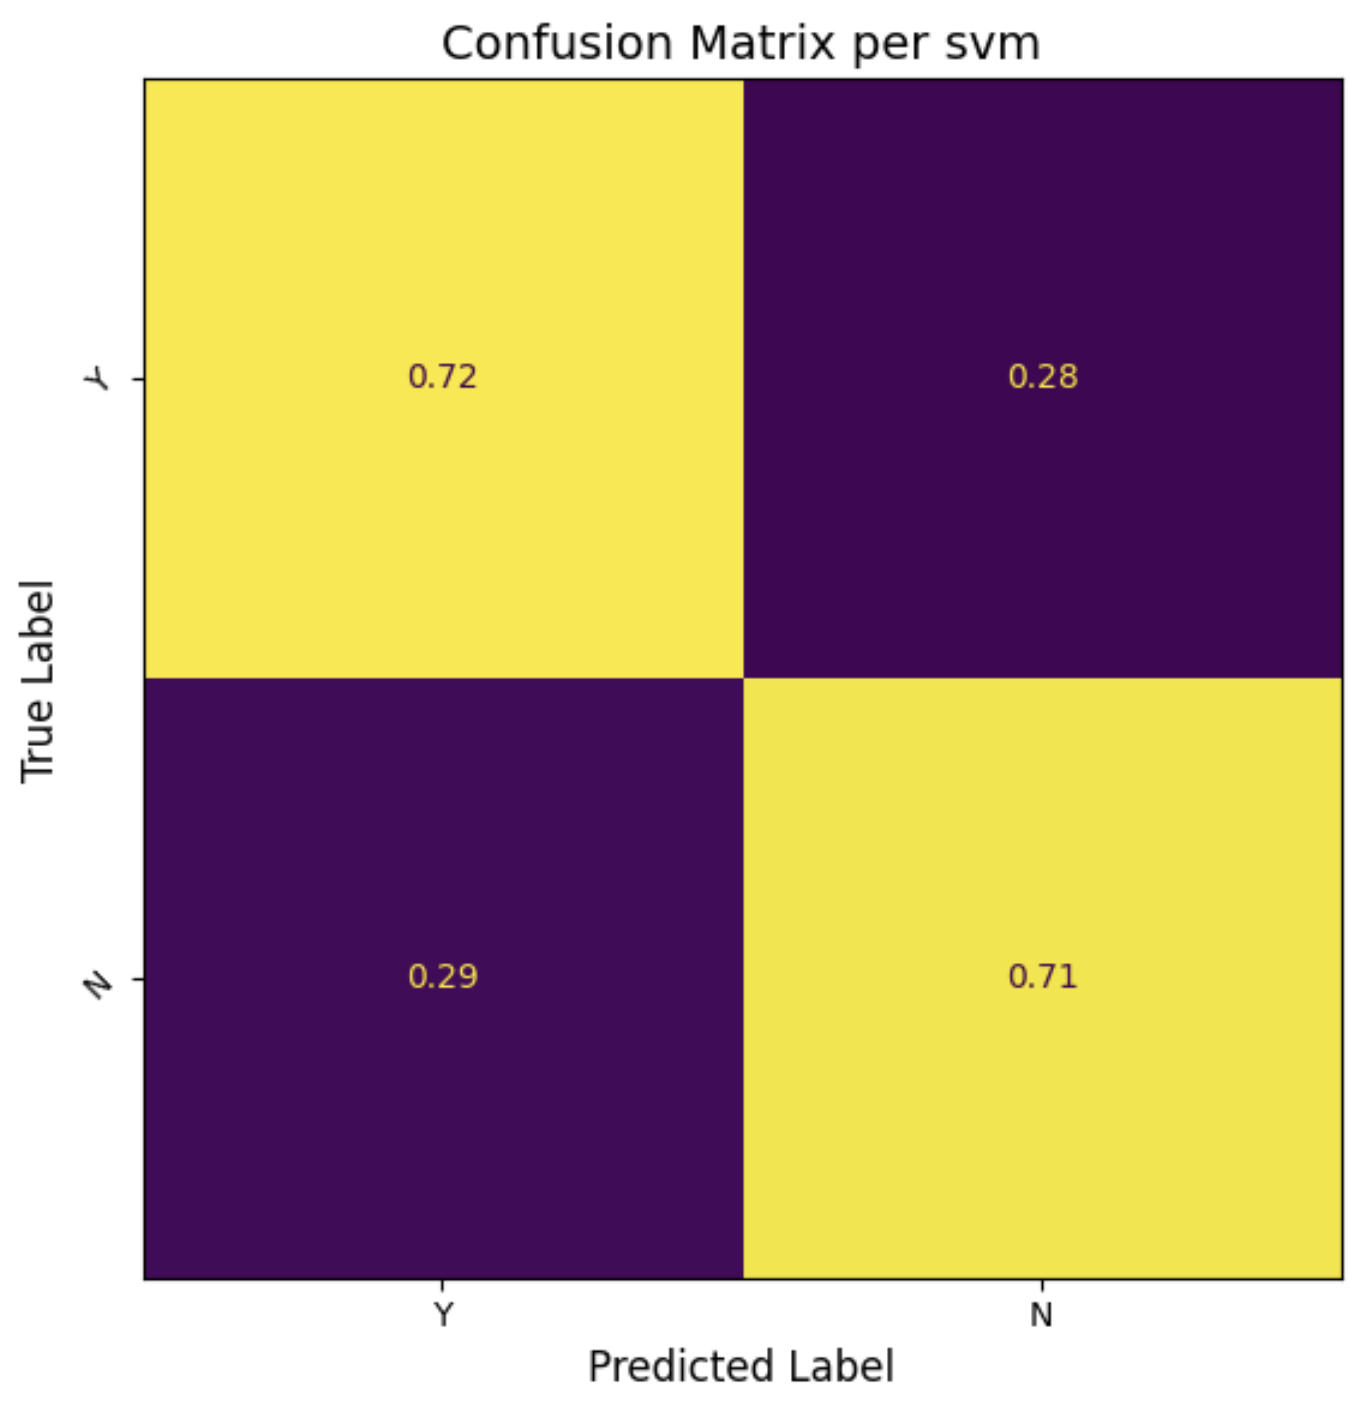
\includegraphics[width=\columnwidth,height=0.75\columnwidth,keepaspectratio]{screen_results/confusion_matrix_svm_pca_d.png}
\end{minipage}
\end{center}

\subsection*{KNN (Drink) }
\begin{center}
\begin{minipage}[c]{0.50\columnwidth}
\resizebox{\columnwidth}{!}{%
\begin{tabular}{lcccc}
\toprule
Label & Precision & Recall & F1-score & Support \\
\midrule
Y     & 0.73      & 0.68   & 0.70     & 99172 \\
N     & 0.70      & 0.75   & 0.72     & 99098 \\
\midrule
Accuracy     & --        & --     & 0.71     & 198270 \\
Macro avg    & 0.71      & 0.71   & 0.71     & 198270 \\
Weighted avg & 0.71      & 0.71   & 0.71     & 198270 \\
\bottomrule
\end{tabular}%
}
\end{minipage}\hspace{\columnsep}%
\begin{minipage}[c]{0.40\columnwidth}
\centering
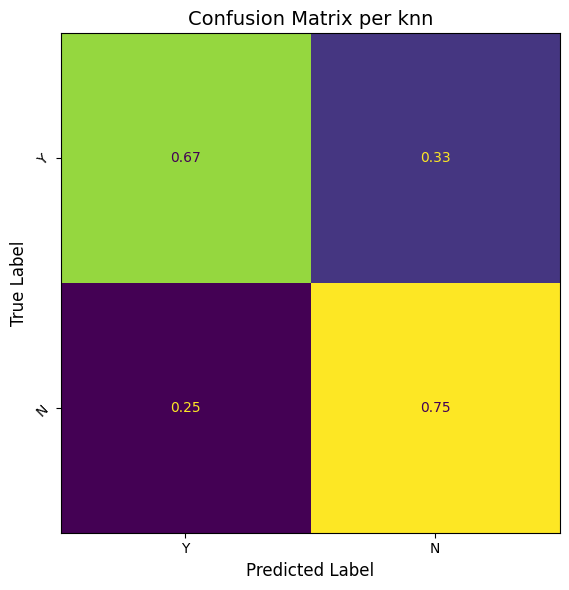
\includegraphics[width=\columnwidth,height=0.75\columnwidth,keepaspectratio]{screen_results/confusion_matrix_knn_pca_d.png}
\end{minipage}
\end{center}

%%%%%%%%%%%%%%%%%%%%%%%%%%%%%%%%%%%%%%%%%%%%%%%%%%%%%%%%%%%%%%%%%%%%%%%%%%%%%%
% Feature Engeneering (Random Forest, AdaBoost, SVM, KNN)
%%%%%%%%%%%%%%%%%%%%%%%%%%%%%%%%%%%%%%%%%%%%%%%%%%%%%%%%%%%%%%%%%%%%%%%%%%%%%%

\subsection{Feature Engeneering (Random Forest, AdaBoost, SVM, KNN)}
Il tentativo di fare feature engeneering, è stato un test che non sapevamo se ed eventualmente in che misura avrebbe influito sui risultati; noi ci siamo limitato ad aggregare le nuove feature ricavate a quelle già esistenti e sicuramente avremmo potuto fare delle prove differenti, per esempio utilizzando solo le nuove feature, oppure facendo feature selection, oppure ancora facendo delle trasformazioni differenti da quelle attuate da noi.
Purtroppo anche in questo caso le performance non sono migliorate rispetto agli step precedenti, però comunque le metriche sono rimaste più o meno invariate, segno che le feature aggiunte non hanno causato overfitting o altri tipi di problemi.

\subsection*{Random Forest (Smoke)}
\begin{center}
\begin{minipage}[c]{0.50\columnwidth}
\resizebox{\columnwidth}{!}{%
\begin{tabular}{lcccc}
\toprule
Label        & Precision & Recall & F1-score & Support \\
\midrule
Non-smoker   & 0.94      & 0.73   & 0.82     & 120489 \\
Ex-smoker    & 0.42      & 0.58   & 0.48     & 34990  \\
Smoker       & 0.49      & 0.64   & 0.56     & 42791  \\
\midrule
Accuracy     & --        & --     & 0.68     & 198270 \\
Macro avg    & 0.62      & 0.65   & 0.62     & 198270 \\
Weighted avg & 0.75      & 0.68   & 0.70     & 198270 \\
\bottomrule
\end{tabular}%
}
\end{minipage}\hspace{\columnsep}%
\begin{minipage}[c]{0.40\columnwidth}
\centering
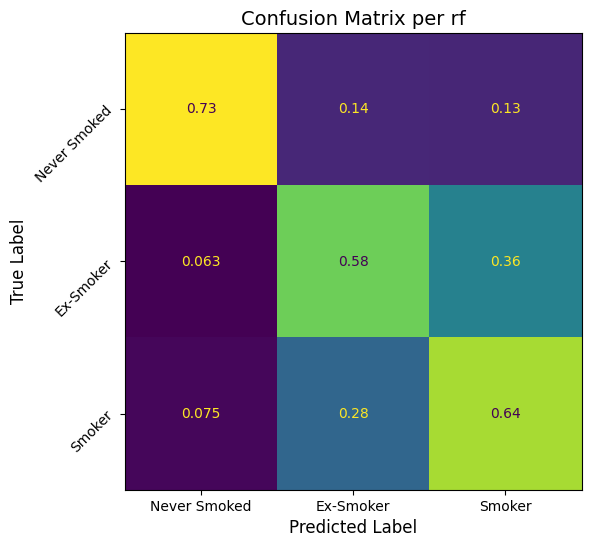
\includegraphics[width=\columnwidth,height=0.75\columnwidth,keepaspectratio]{screen_results/confusion_matrix_feature_engeneering_rf_s.png}
\end{minipage}
\end{center}

\subsection*{AdaBoost (Smoke)}
\begin{center}
\begin{minipage}[c]{0.50\columnwidth}
\resizebox{\columnwidth}{!}{%
\begin{tabular}{lcccc}
\toprule
Label        & Precision & Recall & F1-score & Support \\
\midrule
Non-smoker   & 0.83      & 0.83   & 0.83     & 120489 \\
Ex-smoker    & 0.44      & 0.32   & 0.37     & 34990  \\
Smoker       & 0.51      & 0.62   & 0.56     & 42791  \\
\midrule
Accuracy     & --        & --     & 0.70     & 198270 \\
Macro avg    & 0.59      & 0.59   & 0.59     & 198270 \\
Weighted avg & 0.69      & 0.70   & 0.69     & 198270 \\
\bottomrule
\end{tabular}%
}
\end{minipage}\hspace{\columnsep}%
\begin{minipage}[c]{0.40\columnwidth}
\centering
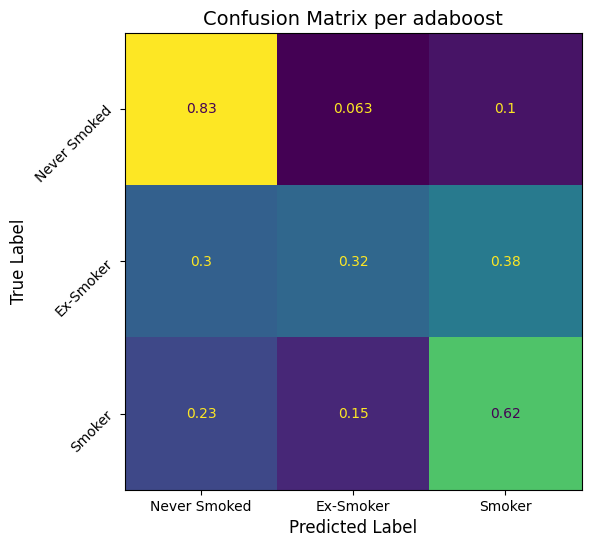
\includegraphics[width=\columnwidth,height=0.75\columnwidth,keepaspectratio]{screen_results/confusion_matrix_feature_engeneering_adaboost_s.png}
\end{minipage}
\end{center}

\subsection*{SVM (Smoke)}
\begin{center}
\begin{minipage}[c]{0.50\columnwidth}
\resizebox{\columnwidth}{!}{%
\begin{tabular}{lcccc}
\toprule
Label        & Precision & Recall & F1-score & Support \\
\midrule
Non-smoker   & 0.94      & 0.73   & 0.82     & 120489 \\
Ex-smoker    & 0.41      & 0.55   & 0.47     & 34990  \\
Smoker       & 0.48      & 0.65   & 0.55     & 42791  \\
\midrule
Accuracy     & --        & --     & 0.68     & 198270 \\
Macro avg    & 0.61      & 0.64   & 0.61     & 198270 \\
Weighted avg & 0.75      & 0.68   & 0.70     & 198270 \\
\bottomrule
\end{tabular}%
}
\end{minipage}\hspace{\columnsep}%
\begin{minipage}[c]{0.40\columnwidth}
\centering
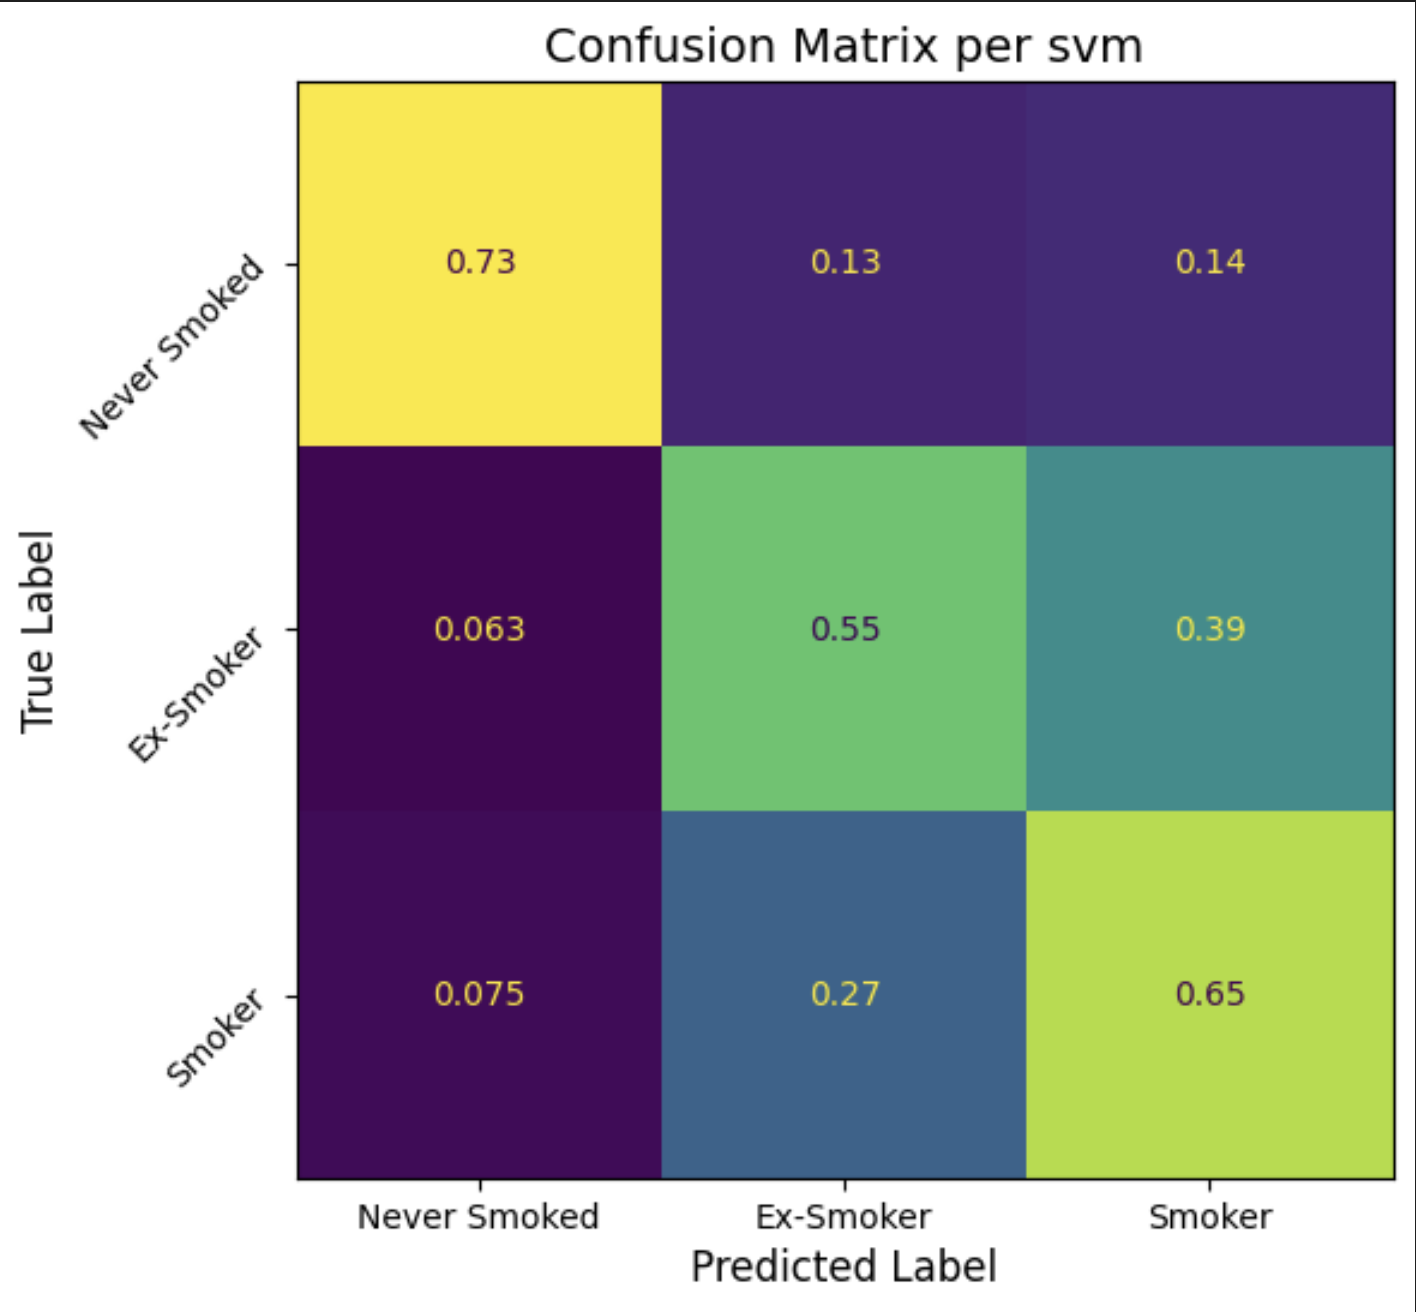
\includegraphics[width=\columnwidth,height=0.75\columnwidth,keepaspectratio]{screen_results/confusion_matrix_feature_engeneering_svm_s.png}
\end{minipage}
\end{center}

\subsection*{KNN (Smoke)}
\begin{center}
\begin{minipage}[c]{0.50\columnwidth}
\resizebox{\columnwidth}{!}{%
\begin{tabular}{lcccc}
\toprule
Label        & Precision & Recall & F1-score & Support \\
\midrule
Non-smoker   & 0.84      & 0.81   & 0.83     & 120489 \\
Ex-smoker    & 0.43      & 0.38   & 0.41     & 34990  \\
Smoker       & 0.49      & 0.58   & 0.53     & 42791  \\
\midrule
Accuracy     & --        & --     & 0.69     & 198270 \\
Macro avg    & 0.59      & 0.59   & 0.59     & 198270 \\
Weighted avg & 0.69      & 0.69   & 0.69     & 198270 \\
\bottomrule
\end{tabular}%
}
\end{minipage}\hspace{\columnsep}%
\begin{minipage}[c]{0.40\columnwidth}
\centering
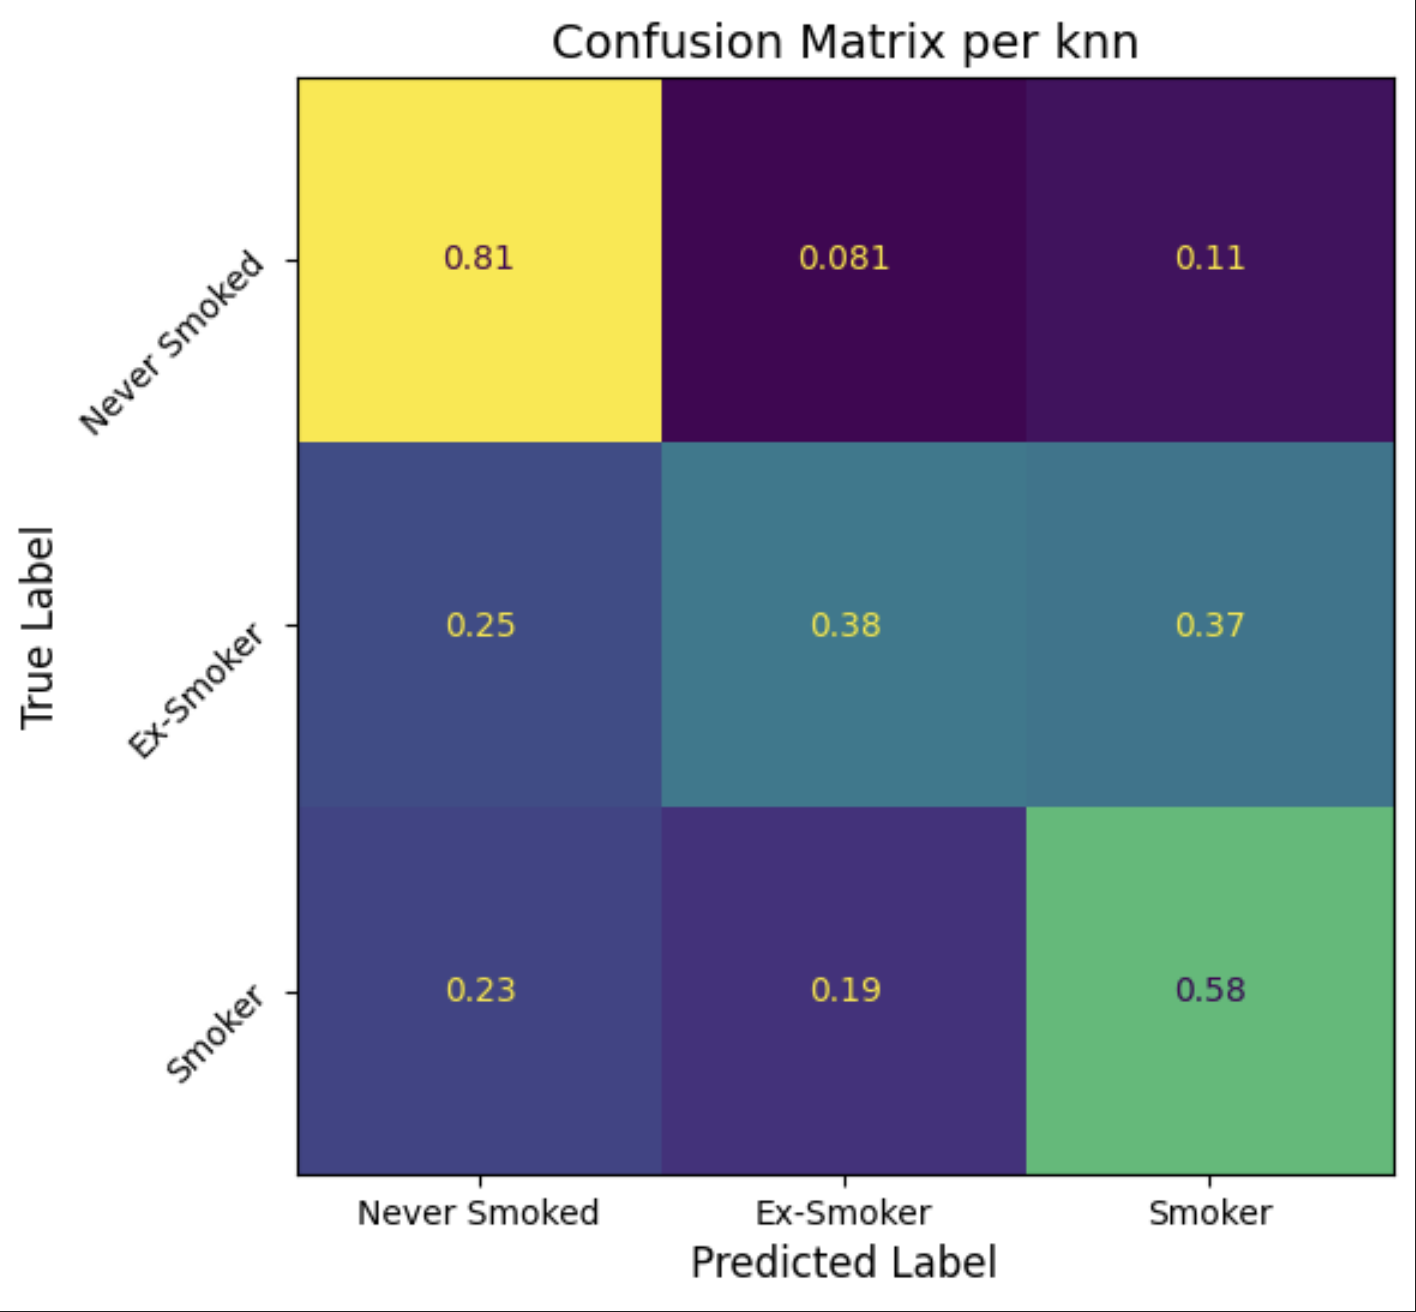
\includegraphics[width=\columnwidth,height=0.75\columnwidth,keepaspectratio]{screen_results/confusion_matrix_feature_engeneering_knn_s.png}
\end{minipage}
\end{center}

\subsection*{Random Forest (Drink)}
\begin{center}
\begin{minipage}[c]{0.50\columnwidth}
\resizebox{\columnwidth}{!}{%
\begin{tabular}{lcccc}
\toprule
Label & Precision & Recall & F1-score & Support \\
\midrule
Y     & 0.74      & 0.72   & 0.73     & 99172 \\
N     & 0.73      & 0.75   & 0.74     & 99098 \\
\midrule
Accuracy     & --        & --     & 0.73     & 198270 \\
Macro avg    & 0.73      & 0.73   & 0.73     & 198270 \\
Weighted avg & 0.73      & 0.73   & 0.73     & 198270 \\
\bottomrule
\end{tabular}%
}
\end{minipage}\hspace{\columnsep}%
\begin{minipage}[c]{0.40\columnwidth}
\centering
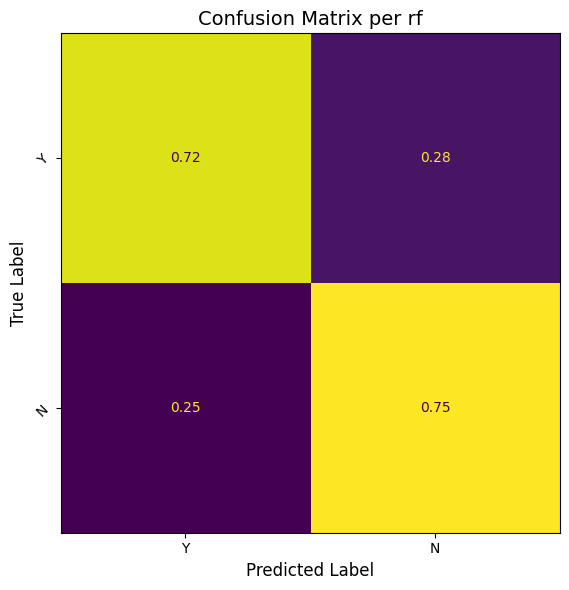
\includegraphics[width=\columnwidth,height=0.75\columnwidth,keepaspectratio]{screen_results/confusion_matrix_feature_engeneering_rf_d.png}
\end{minipage}
\end{center}

\subsection*{AdaBoost (Drink)}
\begin{center}
\begin{minipage}[c]{0.50\columnwidth}
\resizebox{\columnwidth}{!}{%
\begin{tabular}{lcccc}
\toprule
Label & Precision & Recall & F1-score & Support \\
\midrule
Y     & 0.73      & 0.73   & 0.73     & 99172 \\
N     & 0.73      & 0.73   & 0.73     & 99098 \\
\midrule
Accuracy     & --        & --     & 0.73     & 198270 \\
Macro avg    & 0.73      & 0.73   & 0.73     & 198270 \\
Weighted avg & 0.73      & 0.73   & 0.73     & 198270 \\
\bottomrule
\end{tabular}%
}
\end{minipage}\hspace{\columnsep}%
\begin{minipage}[c]{0.40\columnwidth}
\centering
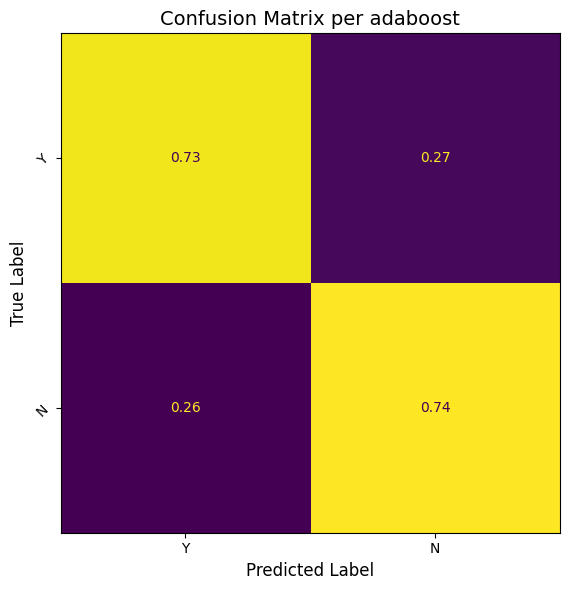
\includegraphics[width=\columnwidth,height=0.75\columnwidth,keepaspectratio]{screen_results/confusion_matrix_feature_engeneering_adaboost_d.png}
\end{minipage}
\end{center}

\subsection*{SVM (Drink)}
\begin{center}
\begin{minipage}[c]{0.50\columnwidth}
\resizebox{\columnwidth}{!}{%
\begin{tabular}{lcccc}
\toprule
Label & Precision & Recall & F1-score & Support \\
\midrule
Y     & 0.73      & 0.72   & 0.72     & 99172 \\
N     & 0.72      & 0.73   & 0.72     & 99098 \\
\midrule
Accuracy     & --        & --     & 0.72     & 198270 \\
Macro avg    & 0.72      & 0.72   & 0.72     & 198270 \\
Weighted avg & 0.72      & 0.72   & 0.72     & 198270 \\
\bottomrule
\end{tabular}%
}
\end{minipage}\hspace{\columnsep}%
\begin{minipage}[c]{0.40\columnwidth}
\centering
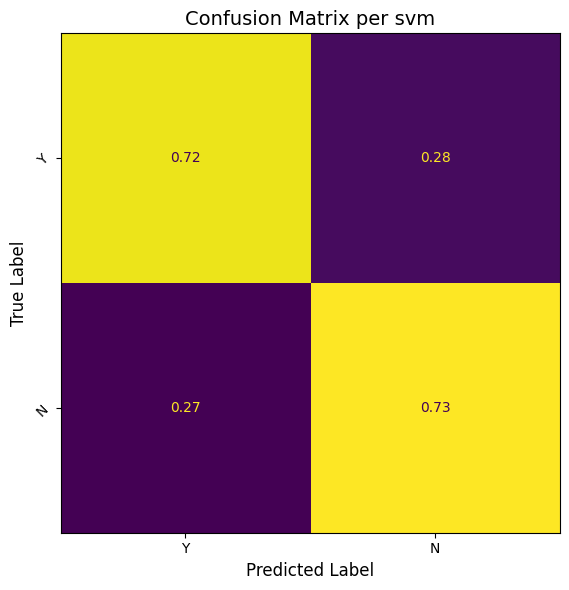
\includegraphics[width=\columnwidth,height=0.75\columnwidth,keepaspectratio]{screen_results/confusion_matrix_feature_engeneering_svm_d.png}
\end{minipage}
\end{center}

\subsection*{KNN (Drink)}
\begin{center}
\begin{minipage}[c]{0.50\columnwidth}
\resizebox{\columnwidth}{!}{%
\begin{tabular}{lcccc}
\toprule
Label & Precision & Recall & F1-score & Support \\
\midrule
Y     & 0.73      & 0.67   & 0.70     & 99172 \\
N     & 0.70      & 0.76   & 0.73     & 99098 \\
\midrule
Accuracy     & --        & --     & 0.71     & 198270 \\
Macro avg    & 0.72      & 0.71   & 0.71     & 198270 \\
Weighted avg & 0.72      & 0.71   & 0.71     & 198270 \\
\bottomrule
\end{tabular}%
}
\end{minipage}\hspace{\columnsep}%
\begin{minipage}[c]{0.40\columnwidth}
\centering
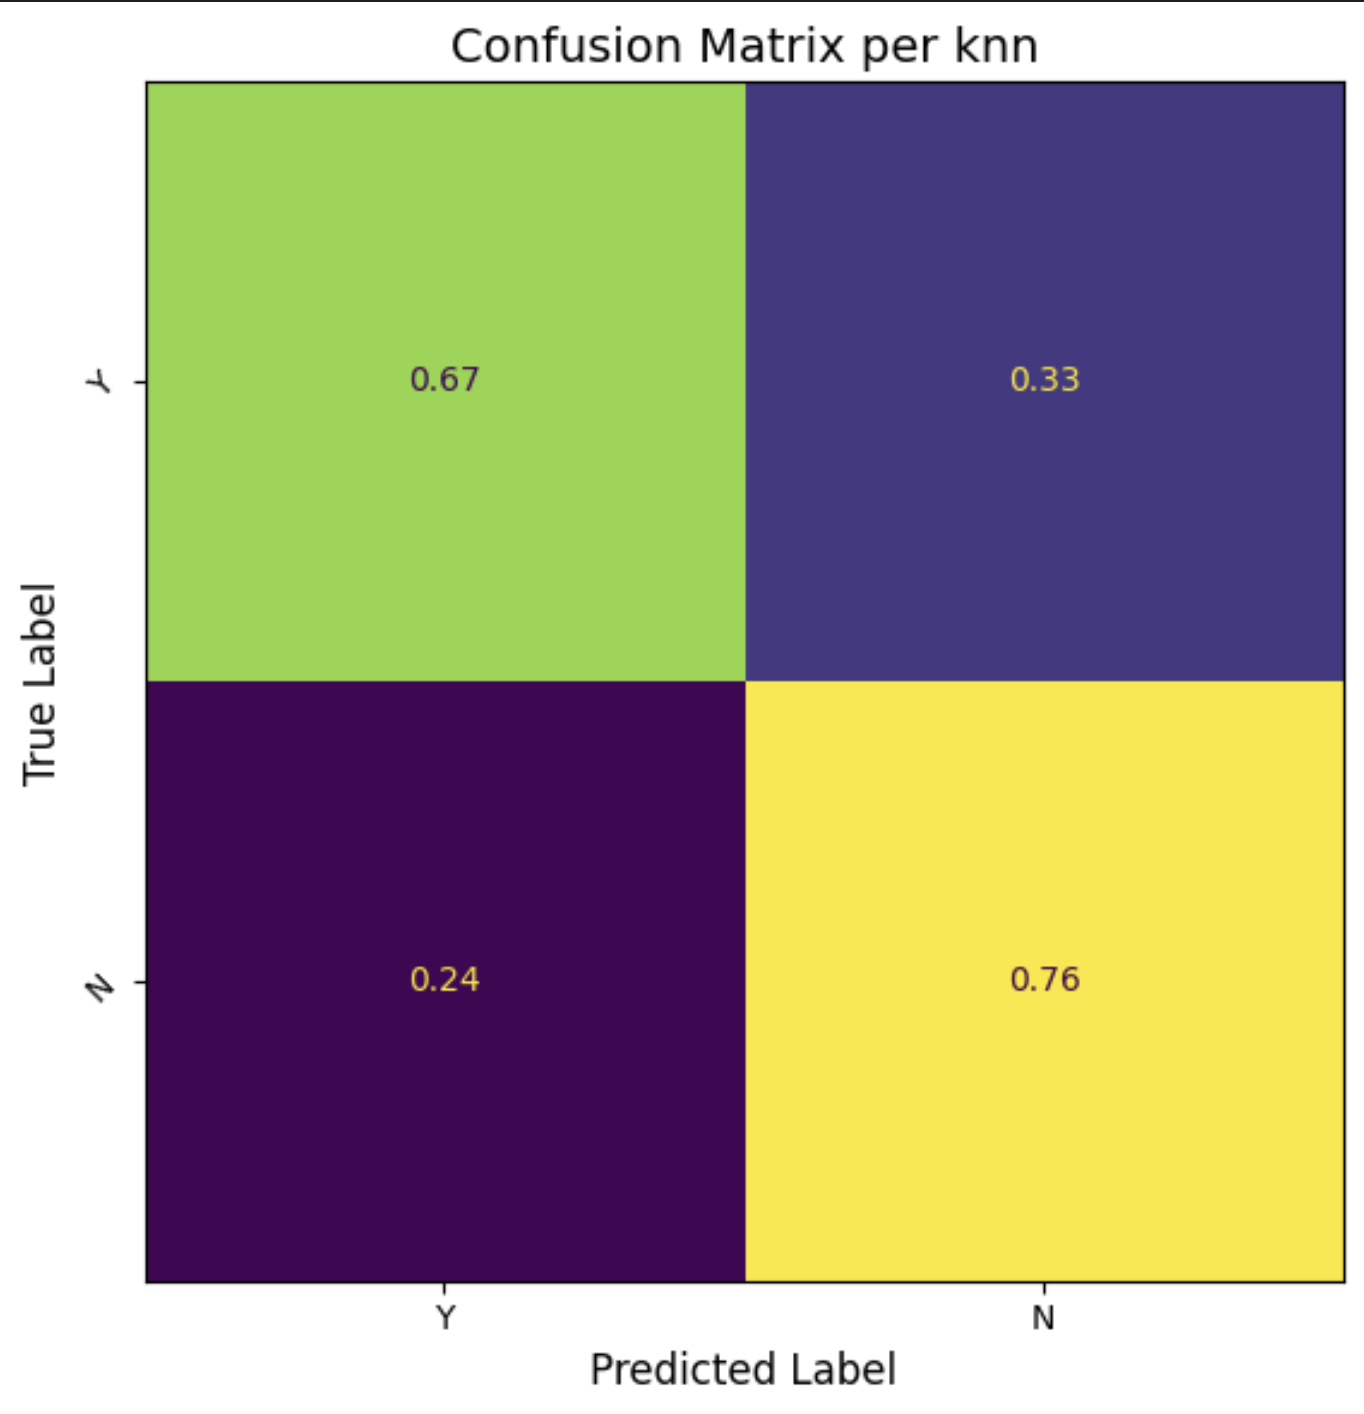
\includegraphics[width=\columnwidth,height=0.75\columnwidth,keepaspectratio]{screen_results/confusion_matrix_feature_engeneering_knn_d.png}
\end{minipage}
\end{center}

%%%%%%%%%%%%%%%%%%%%%%%%%%%%%%%%%%%%%%%%%%%%%%%%%%%%%%%%%%%%%%%%%%%%%%%%%%%%%%
% Feature Engeneering con PCA (SVM, KNN)
%%%%%%%%%%%%%%%%%%%%%%%%%%%%%%%%%%%%%%%%%%%%%%%%%%%%%%%%%%%%%%%%%%%%%%%%%%%%%%

\subsection{Feature Engeneering con PCA (SVM, KNN)}
Per la stessa ragione del caso senza feature engeneering, abbiamo ritenuto opportuno provare ad applicare una PCA ai modelli SVM e KNN; per di più aver aumentato il numero di feature, ha imcrementato la dimensionalità del dataset e dunque abbiamo ritenuto opportuno apllicare una tecnica di dimensionality reduction per cercare di estrarre eventualmente dei pattern più significativi.

\subsection*{SVM (Smoke) }
\begin{center}
\begin{minipage}[c]{0.50\columnwidth}
\resizebox{\columnwidth}{!}{%
\begin{tabular}{lcccc}
\toprule
Label        & Precision & Recall & F1-score & Support \\
\midrule
Non-smoker   & 0.89      & 0.76   & 0.82     & 120489 \\
Ex-smoker    & 0.41      & 0.44   & 0.43     & 34990  \\
Smoker       & 0.48      & 0.63   & 0.54     & 42791  \\
\midrule
Accuracy     & --        & --     & 0.68     & 198270 \\
Macro avg    & 0.59      & 0.61   & 0.60     & 198270 \\
Weighted avg & 0.71      & 0.68   & 0.69     & 198270 \\
\bottomrule
\end{tabular}%
}
\end{minipage}\hspace{\columnsep}%
\begin{minipage}[c]{0.40\columnwidth}
\centering
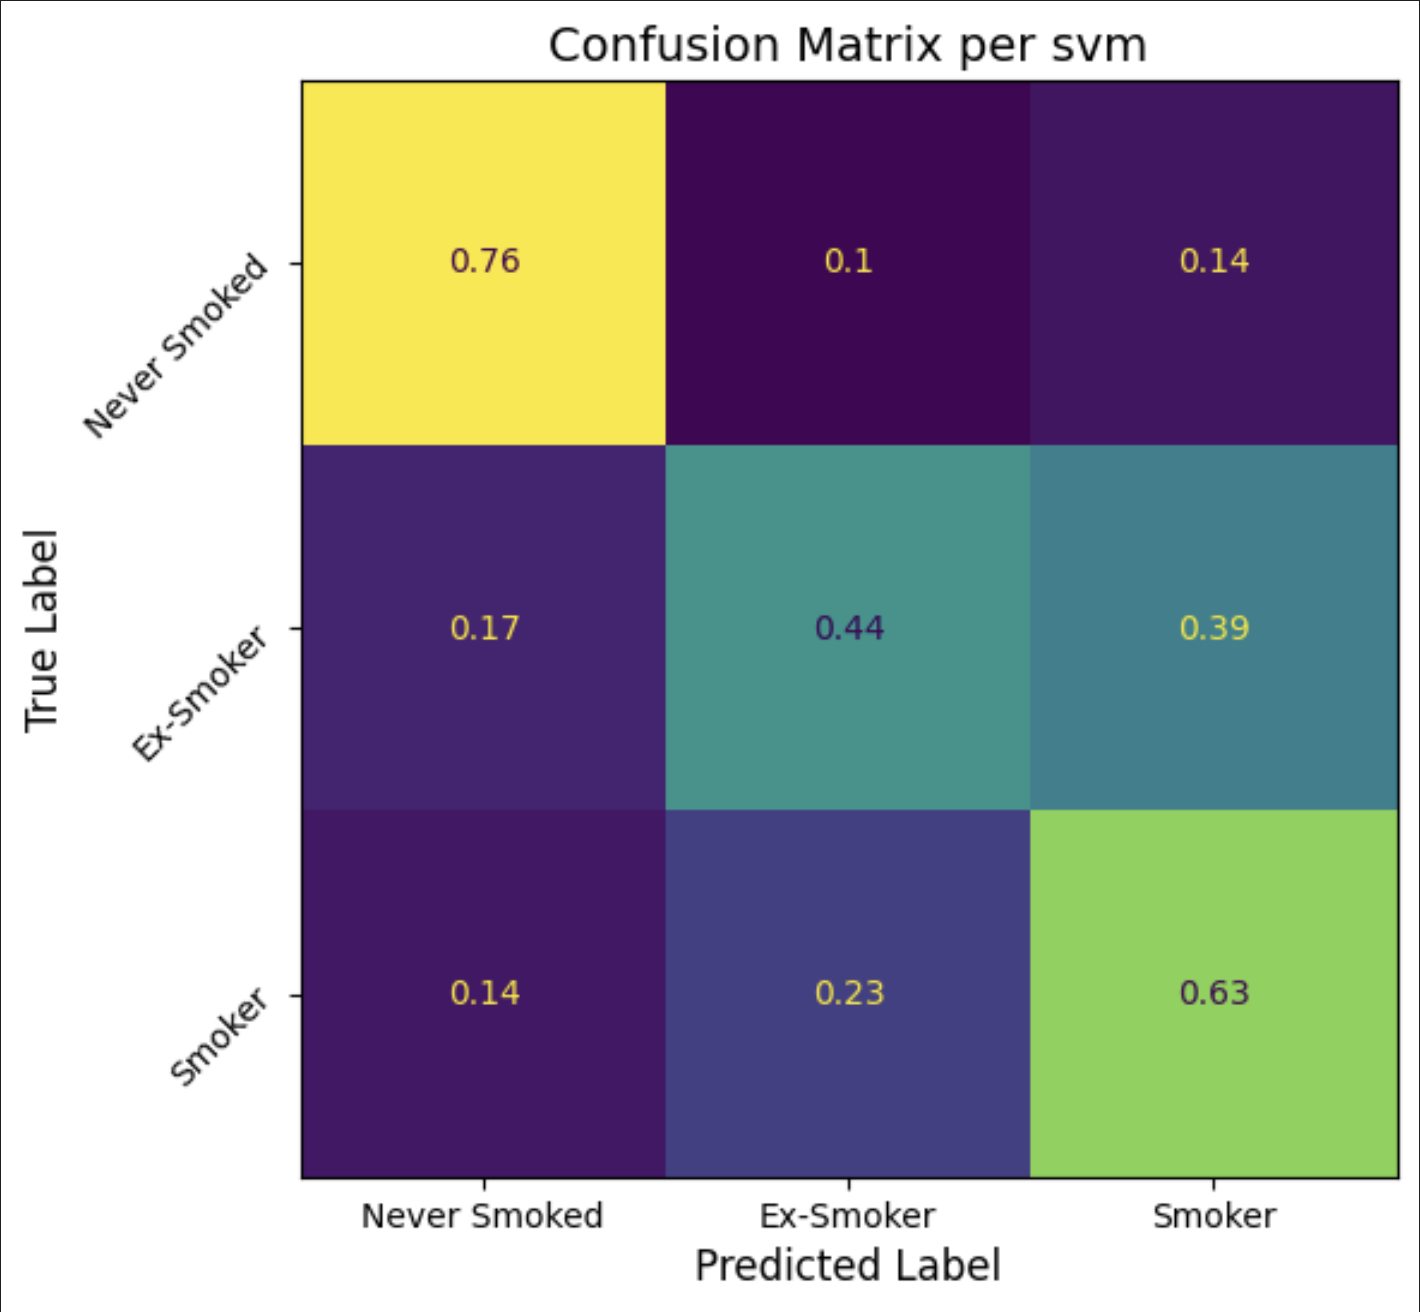
\includegraphics[width=\columnwidth,height=0.75\columnwidth,keepaspectratio]{screen_results/confusion_matrix_feature_engeneering_pca_svm_s.png}
\end{minipage}
\end{center}

\subsection*{KNN (Smoke) }
\begin{center}
\begin{minipage}[c]{0.50\columnwidth}
\resizebox{\columnwidth}{!}{%
\begin{tabular}{lcccc}
\toprule
Label        & Precision & Recall & F1-score & Support \\
\midrule
Non-smoker   & 0.82      & 0.82   & 0.82     & 120489 \\
Ex-smoker    & 0.43      & 0.34   & 0.38     & 34990  \\
Smoker       & 0.49      & 0.57   & 0.53     & 42791  \\
\midrule
Accuracy     & --        & --     & 0.68     & 198270 \\
Macro avg    & 0.58      & 0.58   & 0.58     & 198270 \\
Weighted avg & 0.68      & 0.68   & 0.68     & 198270 \\
\bottomrule
\end{tabular}%
}
\end{minipage}\hspace{\columnsep}%
\begin{minipage}[c]{0.40\columnwidth}
\centering
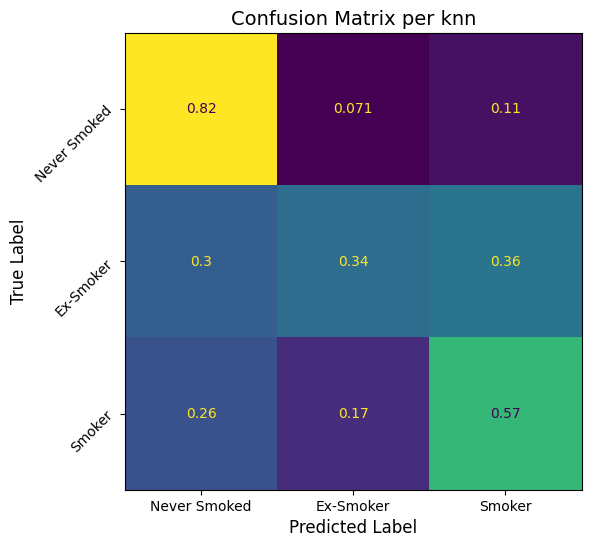
\includegraphics[width=\columnwidth,height=0.75\columnwidth,keepaspectratio]{screen_results/confusion_matrix_feature_engeneering_pca_knn_s.png}
\end{minipage}
\end{center}

\subsection*{SVM (Drink) }
\begin{center}
\begin{minipage}[c]{0.50\columnwidth}
\resizebox{\columnwidth}{!}{%
\begin{tabular}{lcccc}
\toprule
Label & Precision & Recall & F1-score & Support \\
\midrule
Y     & 0.72      & 0.72   & 0.72     & 99172 \\
N     & 0.72      & 0.72   & 0.72     & 99098 \\
\midrule
Accuracy     & --        & --     & 0.72     & 198270 \\
Macro avg    & 0.72      & 0.72   & 0.72     & 198270 \\
Weighted avg & 0.72      & 0.72   & 0.72     & 198270 \\
\bottomrule
\end{tabular}%
}
\end{minipage}\hspace{\columnsep}%
\begin{minipage}[c]{0.40\columnwidth}
\centering
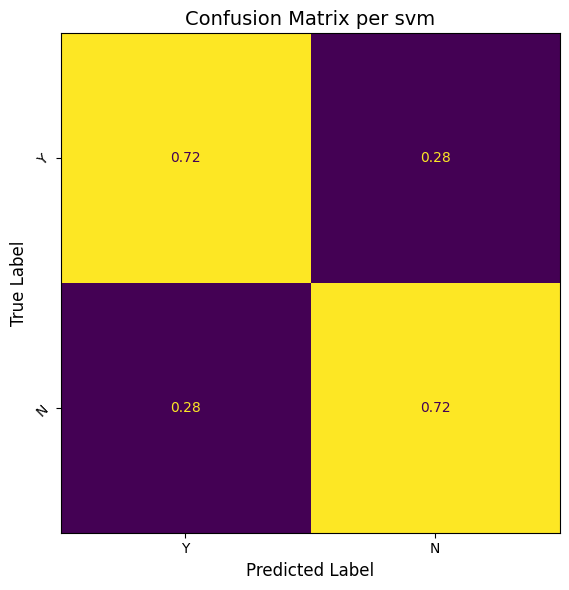
\includegraphics[width=\columnwidth,height=0.75\columnwidth,keepaspectratio]{screen_results/confusion_matrix_feature_engeneering_pca_svm_d.png}
\end{minipage}
\end{center}

\subsection*{KNN (Drink) }
\begin{center}
\begin{minipage}[c]{0.50\columnwidth}
\resizebox{\columnwidth}{!}{%
\begin{tabular}{lcccc}
\toprule
Label & Precision & Recall & F1-score & Support \\
\midrule
Y     & 0.73      & 0.68   & 0.70     & 99172 \\
N     & 0.70      & 0.75   & 0.72     & 99098 \\
\midrule
Accuracy     & --        & --     & 0.71     & 198270 \\
Macro avg    & 0.71      & 0.71   & 0.71     & 198270 \\
Weighted avg & 0.71      & 0.71   & 0.71     & 198270 \\
\bottomrule
\end{tabular}%
}
\end{minipage}\hspace{\columnsep}%
\begin{minipage}[c]{0.40\columnwidth}
\centering
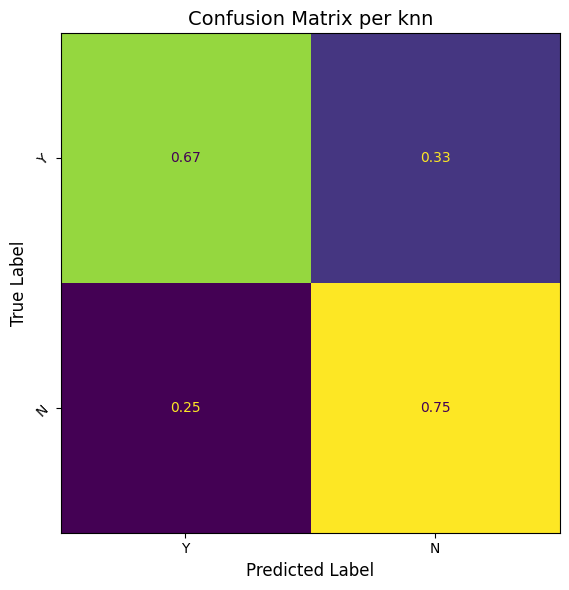
\includegraphics[width=\columnwidth,height=0.75\columnwidth,keepaspectratio]{screen_results/confusion_matrix_knn_pca_d.png}
\end{minipage}
\end{center}

%%%%%%%%%%%%%%%%%%%%%%%%%%%%%%%%%%%%%%%%%%%%%%%%%%%%%%%%%%%%%%%%%%%%%%%%%%%%%%
% Bagging Ensemble
%%%%%%%%%%%%%%%%%%%%%%%%%%%%%%%%%%%%%%%%%%%%%%%%%%%%%%%%%%%%%%%%%%%%%%%%%%%%%%

\subsection{Bagging Ensemble}
Siccome il tempo di train di un modello di tipo SVM con kernel non lineare cresce quadraticamente con la grandezza del dataset, si è reso impossibile testare un modello di questo tipo; come soluzione per provare comunque a osservare se fosse possibile ottenere dei risultati interessanti con tale modello, abbiamo provato utilizzare la tecnica di predizione del Bagging Ensemble.
C'è da specificare che ogni modello base di SVM non lineare è stato allenato solo sul 10\% del dataset, dunque i risultati non sono apprezzabili totalmente.
Inoltre, per testare anche la combinazione della tecnica del Bagging con quella del Boosting, in questo tipo di test abbiamo utilizzato anche il classificatore AdaBoost.

\subsection*{AdaBoost (Smoke)}
\begin{center}
\begin{minipage}[c]{0.50\columnwidth}
\resizebox{\columnwidth}{!}{%
\begin{tabular}{lcccc}
\toprule
Label        & Precision & Recall & F1-score & Support \\
\midrule
Non-smoker   & 0.84      & 0.82   & 0.83     & 120582 \\
Ex-smoker    & 0.44      & 0.27   & 0.34     & 34919  \\
Smoker       & 0.49      & 0.65   & 0.56     & 42769  \\
\midrule
Accuracy     & --        & --     & 0.69     & 198270 \\
Macro avg    & 0.59      & 0.58   & 0.57     & 198270 \\
Weighted avg & 0.69      & 0.69   & 0.68     & 198270 \\
\bottomrule
\end{tabular}%
}
\end{minipage}\hspace{\columnsep}%
\begin{minipage}[c]{0.40\columnwidth}
\centering
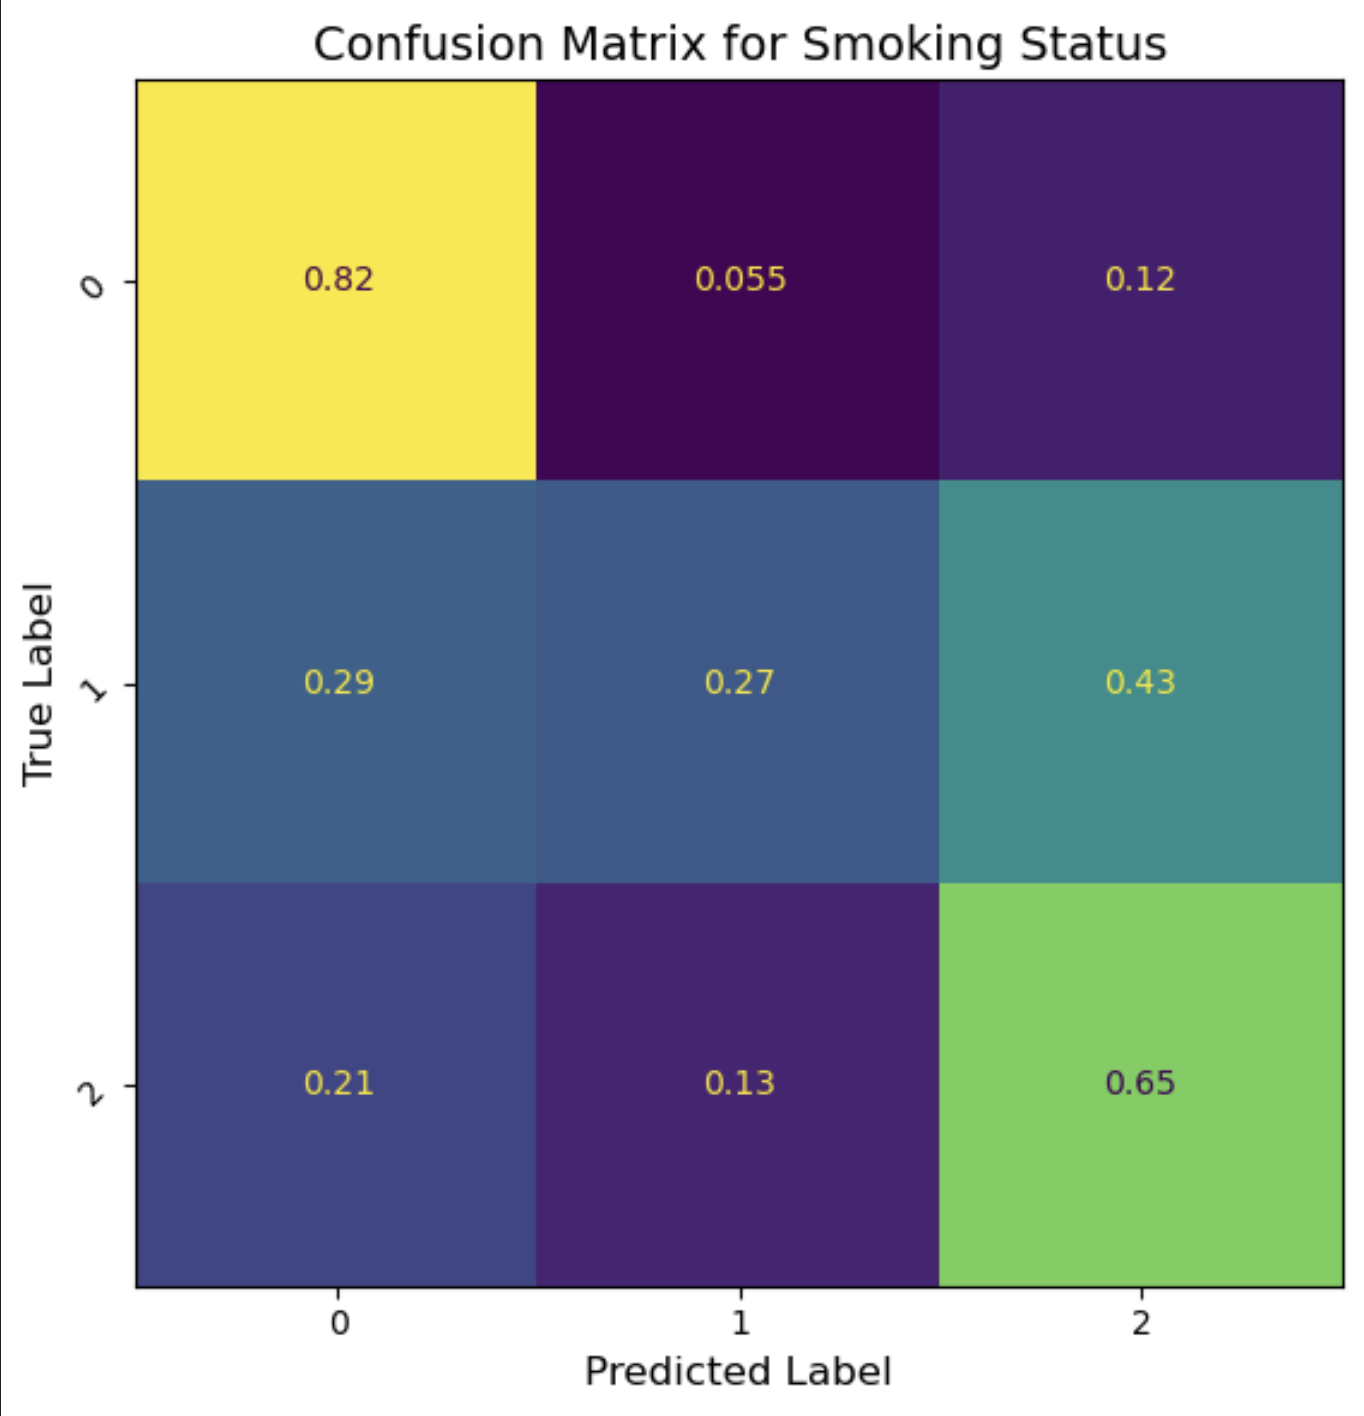
\includegraphics[width=\columnwidth,height=0.75\columnwidth,keepaspectratio]{screen_results/confusion_matrix_bagging_adaboost_s.png}
\end{minipage}
\end{center}

\subsection*{AVM (Smoke)}
\begin{center}
\begin{minipage}[c]{0.50\columnwidth}
\resizebox{\columnwidth}{!}{%
\begin{tabular}{lcccc}
\toprule
Label        & Precision & Recall & F1-score & Support \\
\midrule
Non-smoker   & 0.82      & 0.84   & 0.83     & 120582 \\
Ex-smoker    & 0.45      & 0.31   & 0.37     & 34919  \\
Smoker       & 0.50      & 0.59   & 0.54     & 42769  \\
\midrule
Accuracy     & --        & --     & 0.69     & 198270 \\
Macro avg    & 0.59      & 0.58   & 0.58     & 198270 \\
Weighted avg & 0.68      & 0.69   & 0.68     & 198270 \\
\bottomrule
\end{tabular}%
}
\end{minipage}\hspace{\columnsep}%
\begin{minipage}[c]{0.40\columnwidth}
\centering
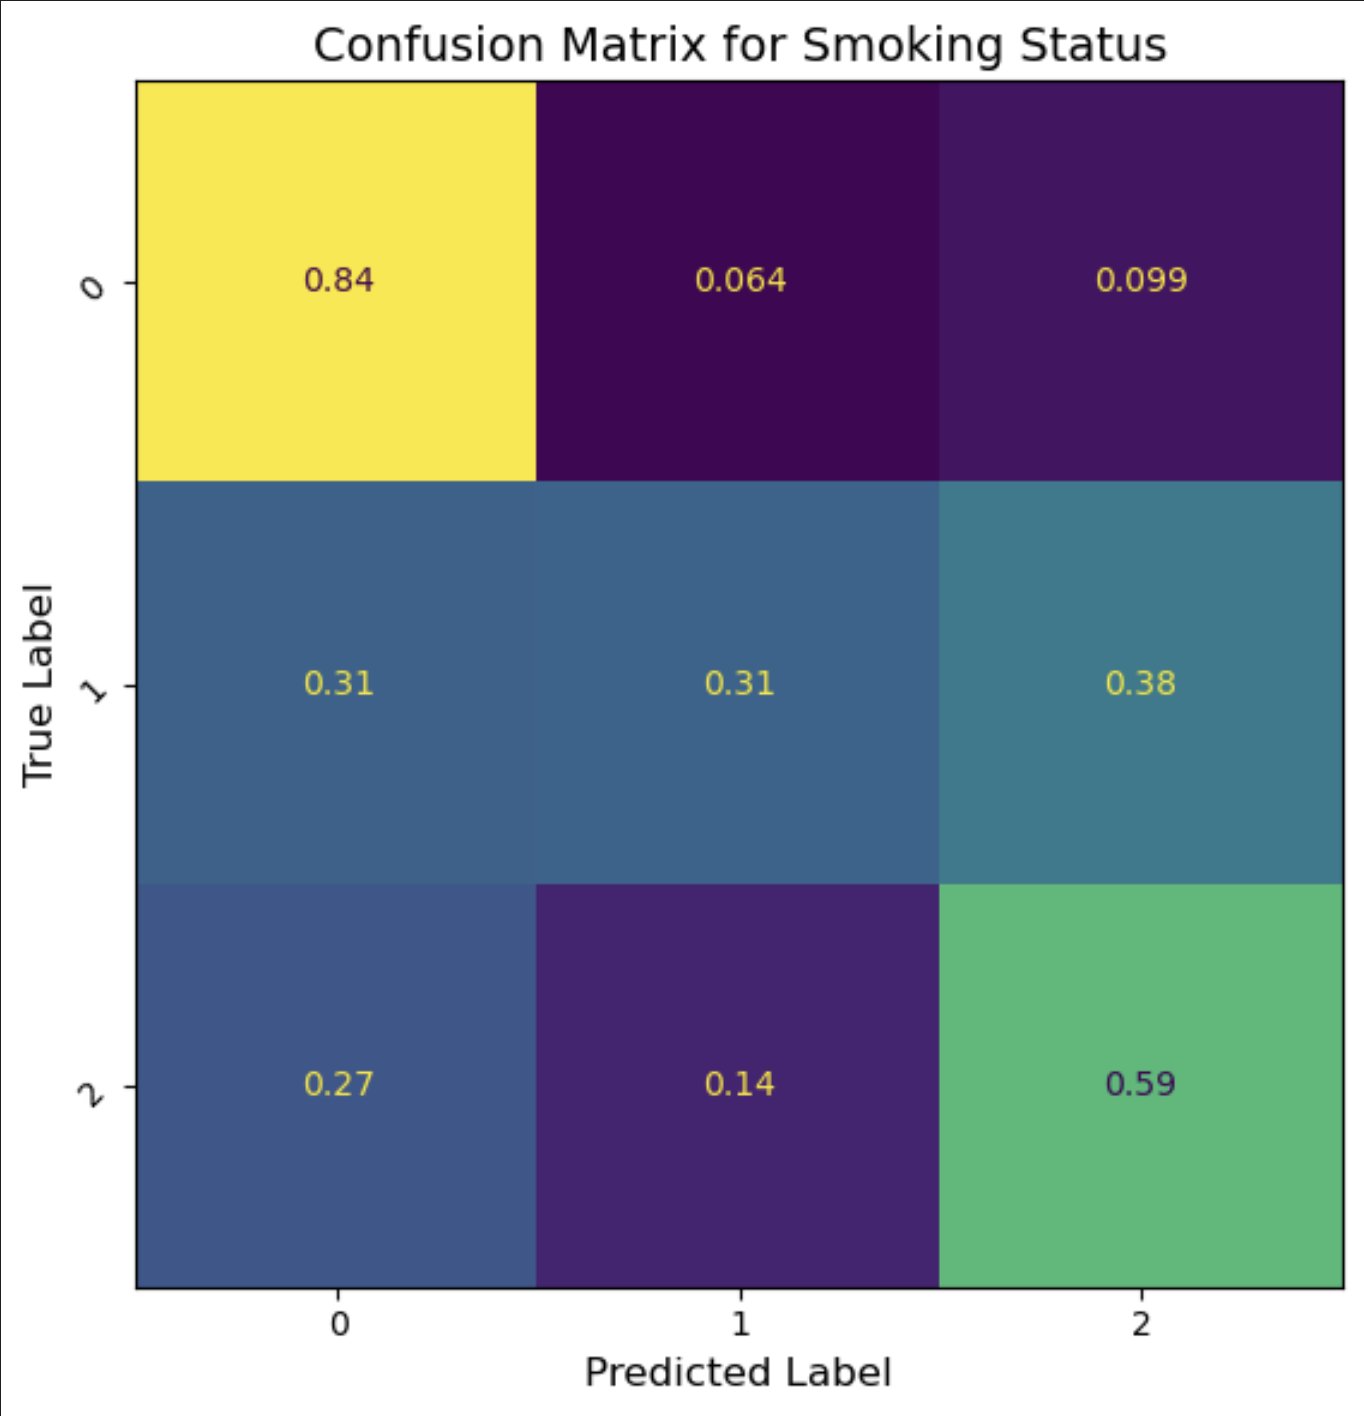
\includegraphics[width=\columnwidth,height=0.75\columnwidth,keepaspectratio]{screen_results/confusion_matrix_bagging_svm_s.png}
\end{minipage}
\end{center}

\subsection*{AdaBoost (Drink)}
\begin{center}
\begin{minipage}[c]{0.50\columnwidth}
\resizebox{\columnwidth}{!}{%
\begin{tabular}{lcccc}
\toprule
Label & Precision & Recall & F1-score & Support \\
\midrule
Y     & 0.72      & 0.73   & 0.72     & 99595 \\
N     & 0.72      & 0.72   & 0.72     & 98675 \\
\midrule
Accuracy     & --        & --     & 0.72     & 198270 \\
Macro avg    & 0.72      & 0.72   & 0.72     & 198270 \\
Weighted avg & 0.72      & 0.72   & 0.72     & 198270 \\
\bottomrule
\end{tabular}%
}
\end{minipage}\hspace{\columnsep}%
\begin{minipage}[c]{0.40\columnwidth}
\centering
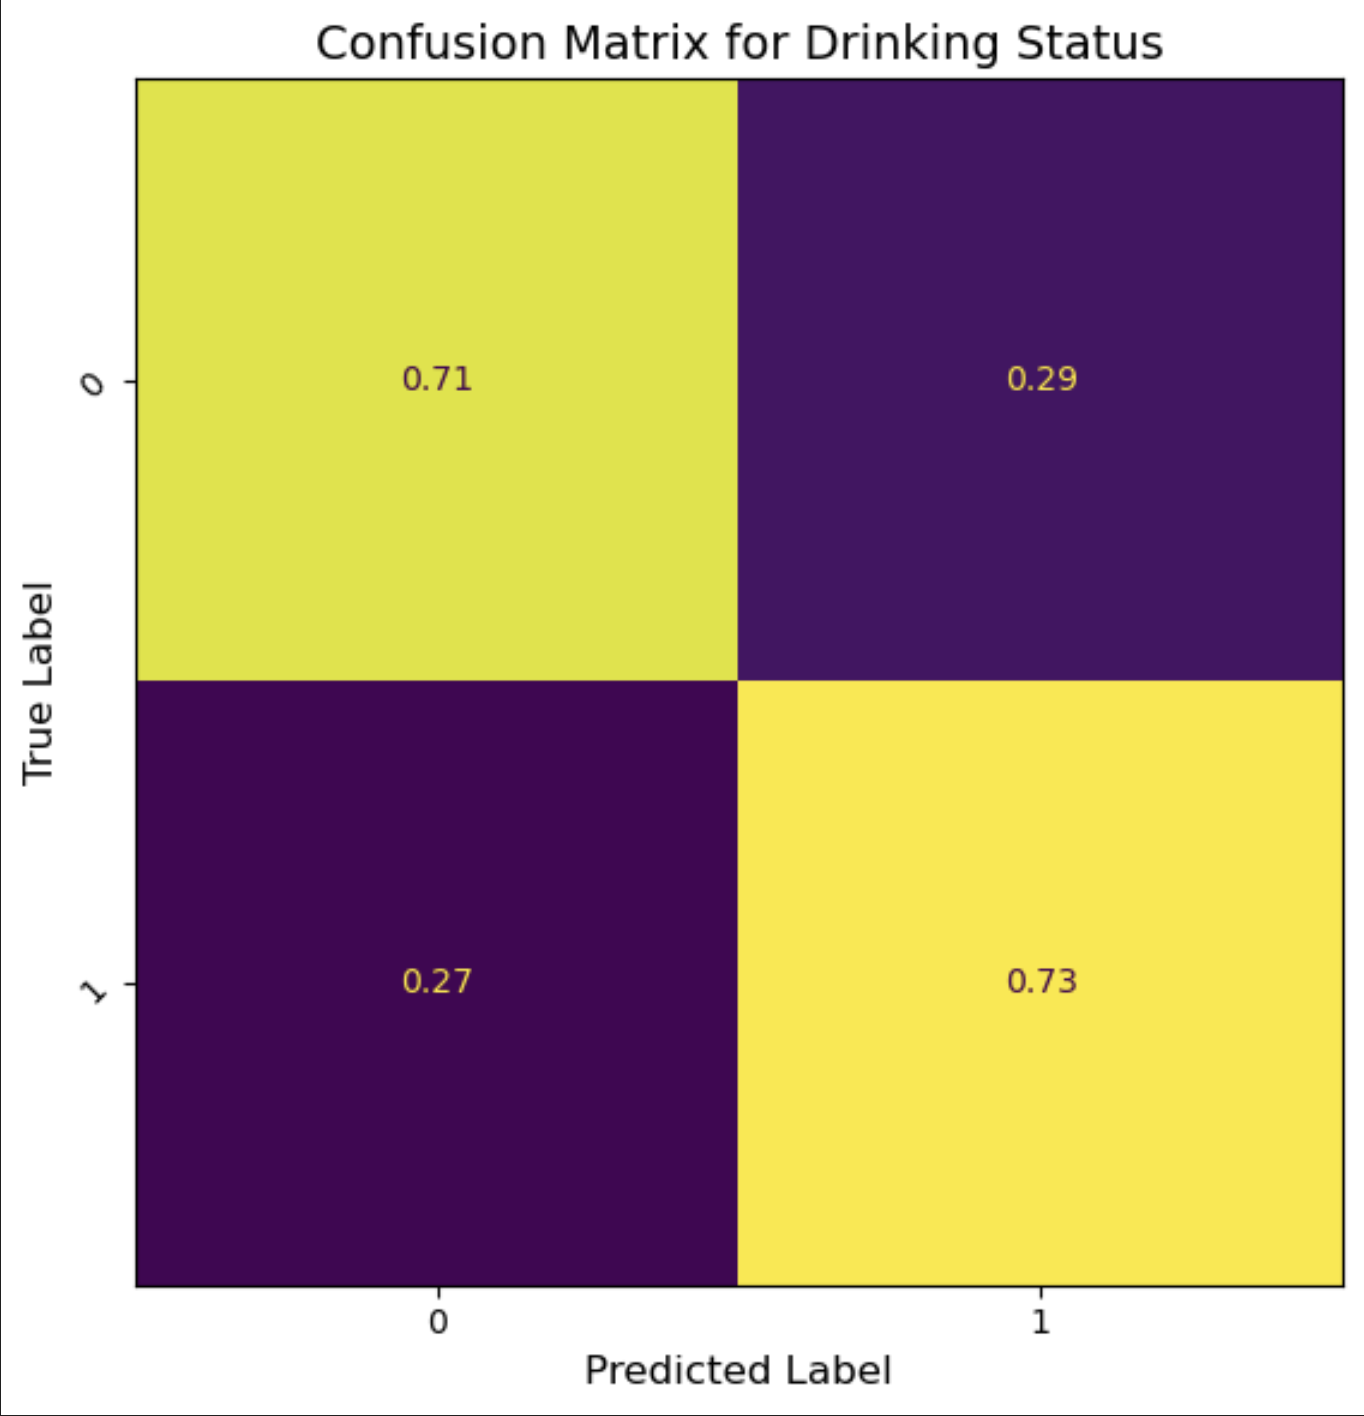
\includegraphics[width=\columnwidth,height=0.75\columnwidth,keepaspectratio]{screen_results/confusion_matrix_bagging_svm_d.png}
\end{minipage}
\end{center}

\subsection*{SVM (Drink)}
\begin{center}
\begin{minipage}[c]{0.50\columnwidth}
\resizebox{\columnwidth}{!}{%
\begin{tabular}{lcccc}
\toprule
Label & Precision & Recall & F1-score & Support \\
\midrule
Y     & 0.73      & 0.71   & 0.72     & 99595 \\
N     & 0.72      & 0.73   & 0.73     & 98675 \\
\midrule
Accuracy     & --        & --     & 0.72     & 198270 \\
Macro avg    & 0.72      & 0.72   & 0.72     & 198270 \\
Weighted avg & 0.72      & 0.72   & 0.72     & 198270 \\
\bottomrule
\end{tabular}%
}
\end{minipage}\hspace{\columnsep}%
\begin{minipage}[c]{0.40\columnwidth}
\centering
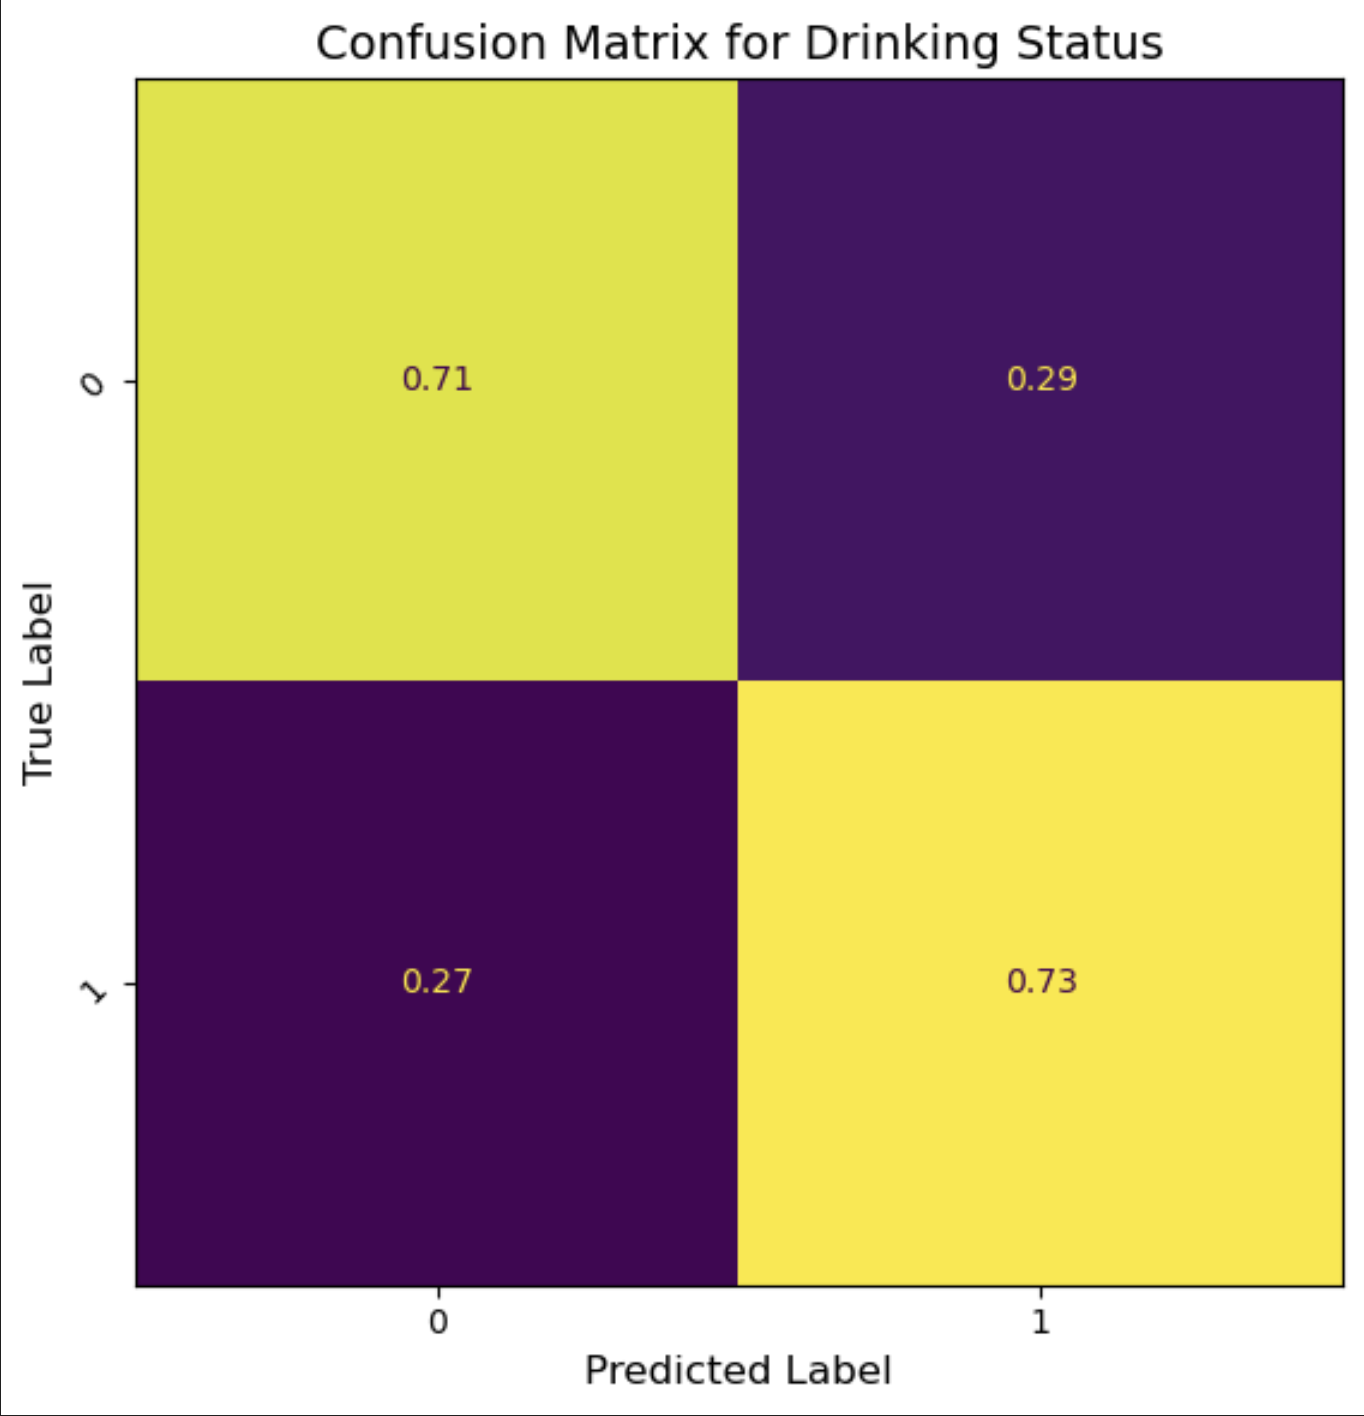
\includegraphics[width=\columnwidth,height=0.75\columnwidth,keepaspectratio]{screen_results/confusion_matrix_bagging_svm_d.png}
\end{minipage}
\end{center}

%%%%%%%%%%%%%%%%%%%%%%%%%%%%%%%%%%%%%%%%%%%%%%%%%%%%%%%%%%%%%%%%%%%%%%%%%%%%%%
% Stacking Classifier e Voting Classifier
%%%%%%%%%%%%%%%%%%%%%%%%%%%%%%%%%%%%%%%%%%%%%%%%%%%%%%%%%%%%%%%%%%%%%%%%%%%%%%

\subsection{Stacking Classifier e Voting Classifier}
Uno dei nostri ultimi tentativi di migliorare i risultati della Random Forest, è stato quello di sfruttare due tecniche di Ensemble differenti dal Bagging ed il Boosting: lo Stacking ed il Voting Classifier; abbiamo pensato infatti che potesse essere conveniente combinare la predizione proveniente da modelli diversi come filosofia, però purtroppo anche per quanto riguarda questo test abbiamo ottenuto più o meno gli stessi risultati.

\subsection*{Stacking (Smoke)}
\begin{center}
\begin{minipage}[c]{0.50\columnwidth}
\resizebox{\columnwidth}{!}{%
\begin{tabular}{lcccc}
\toprule
Label        & Precision & Recall & F1-score & Support \\
\midrule
Non-smoker   & 0.89      & 0.79   & 0.83     & 111686 \\
Ex-smoker    & 0.44      & 0.44   & 0.44     & 31585  \\
Smoker       & 0.50      & 0.66   & 0.57     & 39049  \\
\midrule
Accuracy     & --        & --     & 0.70     & 182320 \\
Macro avg    & 0.61      & 0.63   & 0.61     & 182320 \\
Weighted avg & 0.73      & 0.70   & 0.71     & 182320 \\
\bottomrule
\end{tabular}%
}
\end{minipage}\hspace{\columnsep}%
\begin{minipage}[c]{0.40\columnwidth}
\centering
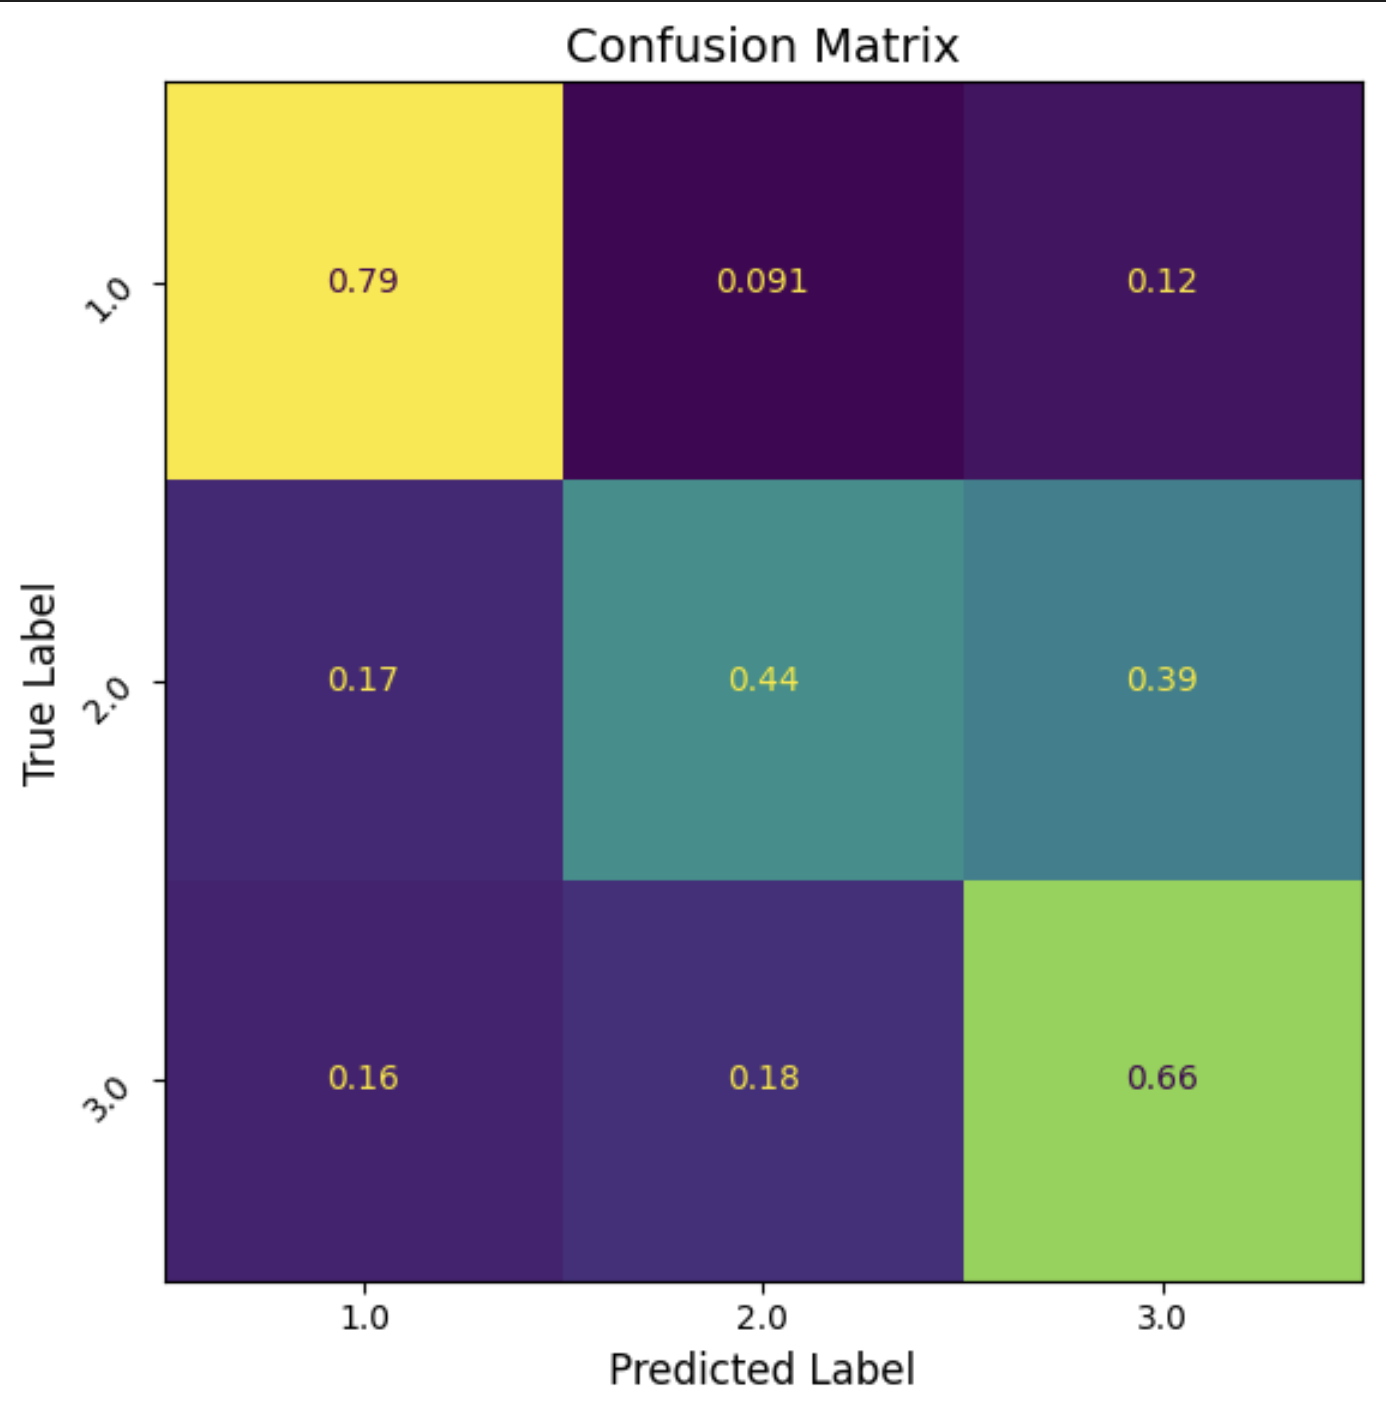
\includegraphics[width=\columnwidth,height=0.75\columnwidth,keepaspectratio]{screen_results/confusion_matrix_stacking_s.png}
\end{minipage}
\end{center}

\subsection*{Voting (Smoke)}
\begin{center}
\begin{minipage}[c]{0.50\columnwidth}
\resizebox{\columnwidth}{!}{%
\begin{tabular}{lcccc}
\toprule
Label        & Precision & Recall & F1-score & Support \\
\midrule
Non-smoker   & 0.93      & 0.74   & 0.83     & 111686 \\
Ex-smoker    & 0.43      & 0.53   & 0.47     & 31585  \\
Smoker       & 0.48      & 0.66   & 0.56     & 39049  \\
\midrule
Accuracy     & --        & --     & 0.69     & 182320 \\
Macro avg    & 0.61      & 0.65   & 0.62     & 182320 \\
Weighted avg & 0.75      & 0.69   & 0.71     & 182320 \\
\bottomrule
\end{tabular}%
}
\end{minipage}\hspace{\columnsep}%
\begin{minipage}[c]{0.40\columnwidth}
\centering
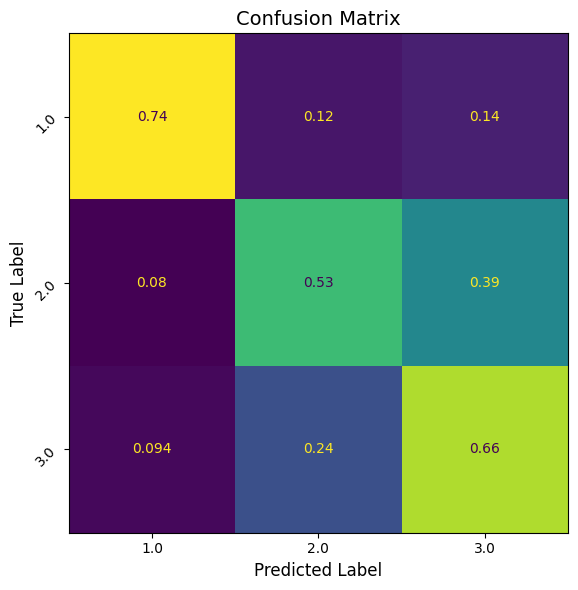
\includegraphics[width=\columnwidth,height=0.75\columnwidth,keepaspectratio]{screen_results/confusion_matrix_voting_s.png}
\end{minipage}
\end{center}

\subsection*{Stacking (Drink)}
\begin{center}
\begin{minipage}[c]{0.50\columnwidth}
\resizebox{\columnwidth}{!}{%
\begin{tabular}{lcccc}
\toprule
Label & Precision & Recall & F1-score & Support \\
\midrule
Y     & 0.73      & 0.71   & 0.72     & 90360 \\
N     & 0.72      & 0.74   & 0.73     & 91960 \\
\midrule
Accuracy     & --        & --     & 0.73     & 182320 \\
Macro avg    & 0.73      & 0.73   & 0.73     & 182320 \\
Weighted avg & 0.73      & 0.73   & 0.73     & 182320 \\
\bottomrule
\end{tabular}%
}
\end{minipage}\hspace{\columnsep}%
\begin{minipage}[c]{0.40\columnwidth}
\centering
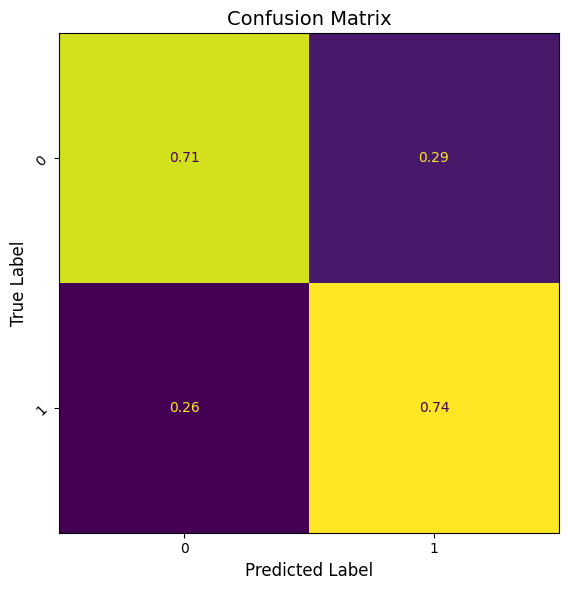
\includegraphics[width=\columnwidth,height=0.75\columnwidth,keepaspectratio]{screen_results/confusion_matrix_stacking_d.png}
\end{minipage}
\end{center}

\subsection*{Voting (Drink)}
\begin{center}
\begin{minipage}[c]{0.50\columnwidth}
\resizebox{\columnwidth}{!}{%
\begin{tabular}{lcccc}
\toprule
Label & Precision & Recall & F1-score & Support \\
\midrule
Y     & 0.74      & 0.68   & 0.71     & 90360 \\
N     & 0.71      & 0.76   & 0.73     & 91960 \\
\midrule
Accuracy     & --        & --     & 0.72     & 182320 \\
Macro avg    & 0.72      & 0.72   & 0.72     & 182320 \\
Weighted avg & 0.72      & 0.72   & 0.72     & 182320 \\
\bottomrule
\end{tabular}%
}
\end{minipage}\hspace{\columnsep}%
\begin{minipage}[c]{0.40\columnwidth}
\centering
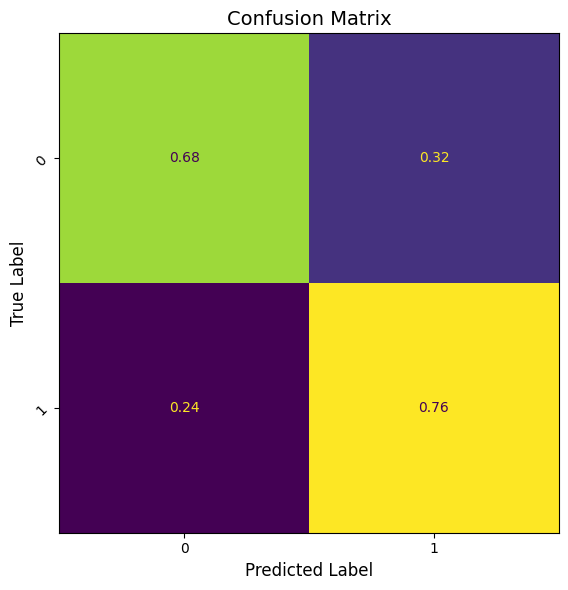
\includegraphics[width=\columnwidth,height=0.75\columnwidth,keepaspectratio]{screen_results/confusion_matrix_voting_d.png}
\end{minipage}
\end{center}

%%%%%%%%%%%%%%%%%%%%%%%%%%%%%%%%%%%%%%%%%%%%%%%%%%%%%%%%%%%%%%%%%%%%%%%%%%%%%%
% Classificatore Gerarchico (Smoke)
%%%%%%%%%%%%%%%%%%%%%%%%%%%%%%%%%%%%%%%%%%%%%%%%%%%%%%%%%%%%%%%%%%%%%%%%%%%%%%

\subsection{Classificatore Gerarchico (Smoke)}
Per quanto riguarda la classificazione sul fumo, che alla fine è stato al centro del nostro progetto più della classificazione sull'alcool, abbiamo fatto un ultimo tentativo per cercare di ottenere un modello di predizione che migliorasse le metriche ottenute fino a questo punto, implementando un classificatore gerarchico; purtoppo, come già accennato nella sezione relativa alla spiegazione dei modelli utilizzati nel progetto non siamo riusciti nel nostro intento per verie ragioni, anche se il risultato finale si avvicina molto alle performance ottenute dal modello Random Forest.
C'è però da fare una precisazione: nonostante questo modello di classificazione gerarchica non sia stato creato come era nostro intento, siamo convinti che la filosofia di creare un modello predittivo di questo tipo sia la carta vincente per poter ottenere il miglior modello possibile per questo tipo di dataset.
Idealmente, infatti, allenando prima un modello che separi nel miglior modo possibile le classi "Non-fumatore" e "Ex-fumatore o Fumatore" ed in un secondo momento un modello che sappia separare meglio possibile le classi "Ex-fumatore" e "Fumatore" si dovrebbe riuscire ad ottenere una "pipeline" che sia in grado di occuparsi step by step della suddivisione dei sample.



\subsection*{Stage 1 --- Non-smokers vs. Ex-/Smokers}
\begin{center}
\begin{minipage}[c]{0.50\columnwidth}
\resizebox{\columnwidth}{!}{%
\begin{tabular}{lcccc}
\toprule
Label         & Precision & Recall & F1-score & Support \\
\midrule
Non-smoker    & 0.93      & 0.75   & 0.83     & 111686 \\
Ex-/Smokers   & 0.69      & 0.91   & 0.79     & 70634  \\
\midrule
Accuracy     & --        & --     & 0.81     & 182320 \\
Macro avg    & 0.81      & 0.83   & 0.81     & 182320 \\
Weighted avg & 0.84      & 0.81   & 0.81     & 182320 \\
\bottomrule
\end{tabular}%
}
\end{minipage}\hspace{\columnsep}%
\begin{minipage}[c]{0.40\columnwidth}
\centering
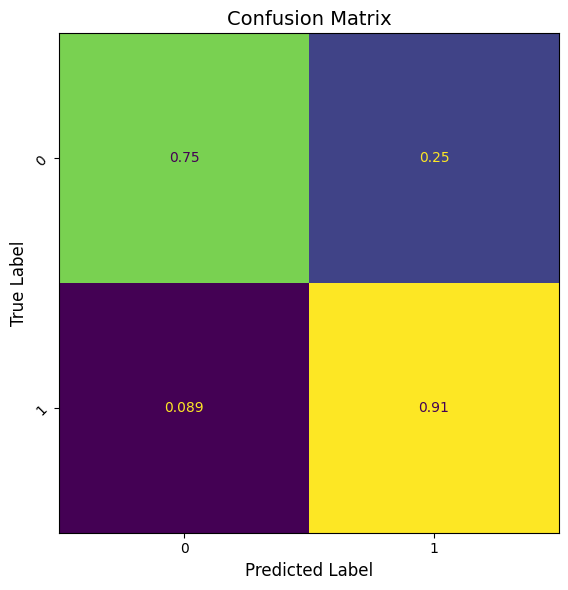
\includegraphics[width=\columnwidth,height=0.75\columnwidth,keepaspectratio]{screen_results/confusion_matrix_separation1.png}
\end{minipage}
\end{center}

\subsection*{Stage 2 --- Ex-smokers vs. Smokers}
\begin{center}
\begin{minipage}[c]{0.50\columnwidth}
\resizebox{\columnwidth}{!}{%
\begin{tabular}{lcccc}
\toprule
Label      & Precision & Recall & F1-score & Support \\
\midrule
Ex-smoker  & 0.62      & 0.60   & 0.61     & 31585  \\
Smoker     & 0.68      & 0.71   & 0.70     & 39049  \\
\midrule
Accuracy     & --        & --     & 0.66     & 70634  \\
Macro avg    & 0.65      & 0.65   & 0.65     & 70634  \\
Weighted avg & 0.66      & 0.66   & 0.66     & 70634  \\
\bottomrule
\end{tabular}%
}
\end{minipage}\hspace{\columnsep}%
\begin{minipage}[c]{0.40\columnwidth}
\centering
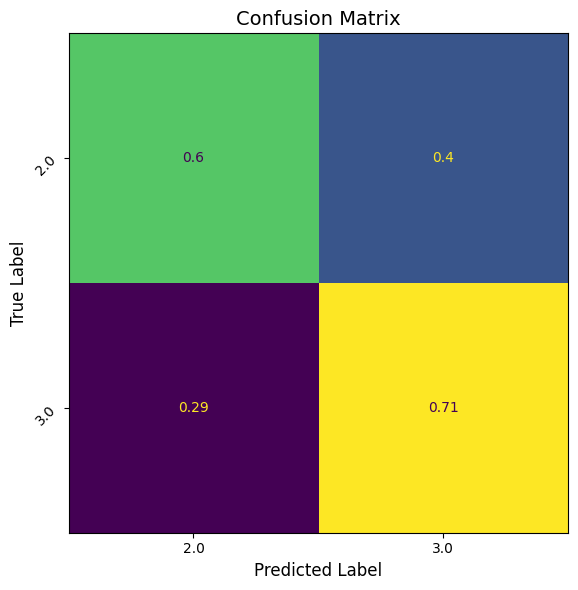
\includegraphics[width=\columnwidth,height=0.75\columnwidth,keepaspectratio]{screen_results/confusion_matrix_separation2.png}
\end{minipage}
\end{center}

\subsection*{Test Classificatore Gerarchico}
\begin{center}
\begin{minipage}[c]{0.50\columnwidth}
\resizebox{\columnwidth}{!}{%
\begin{tabular}{lcccc}
\toprule
Label        & Precision & Recall & F1-score & Support \\
\midrule
Non-smoker   & 0.94      & 0.73   & 0.82     & 111704 \\
Ex-smoker    & 0.41      & 0.55   & 0.47     & 31616  \\
Smoker       & 0.48      & 0.65   & 0.55     & 39085  \\
\midrule
Accuracy     & --        & --     & 0.68     & 182405 \\
Macro avg    & 0.61      & 0.64   & 0.61     & 182405 \\
Weighted avg & 0.75      & 0.68   & 0.70     & 182405 \\
\bottomrule
\end{tabular}%
}
\end{minipage}\hspace{\columnsep}%
\begin{minipage}[c]{0.40\columnwidth}
\centering
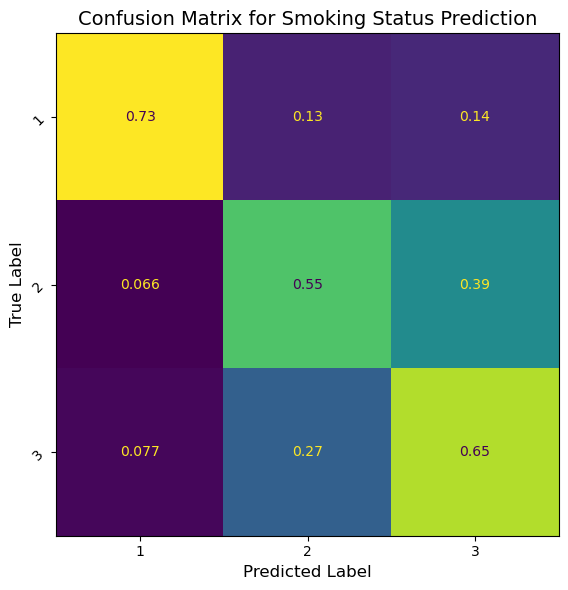
\includegraphics[width=\columnwidth,height=0.75\columnwidth,keepaspectratio]{screen_results/confusion_matrix_multistep_s.png}
\end{minipage}
\end{center}

\newpage

\subsection{Visualizzazione della Separazione delle Classi}

Di seguito vengono riportate le distribuzioni nello spazio dei dati presenti nel dataset, ottenuti sfruttando le tecniche di t-SNE e PCA; in questo modo abbiamo potuto visualizzare quanto effettivamente le classi del nostro dataset fossero sovrapposte tra di loro. 
Ovviamente per rendere il tutto più comprensibile, abbiamo "plottato" il tutto in uno spazio a 2 dimensioni e considerando in un primo momento le label "Non-fumatore" e "Ex-fumatore o Fumatore" accorpate in una unica classe ed in un secondo momento le classi "Ex-fumatore" e "Fumatore". 
Come si può vedere, la divisione "Non-fumatore" e "Ex-fumatore o Fumatore" è abbastanza marcata e facile da individuare, mentre per l'altra divisione si nota una netta sovrapposizione dei dati delle due classi, marcando dunque la difficoltà nel riuscire a distinguere in maniera anche solo parziale le due classi. 
Per ottenere risultati in tempi contenuti, abbiamo utilizzato solo il 10\% del dataset.

\begin{figure}[h]
    \centering
    \begin{minipage}{0.45\textwidth}
        \centering
        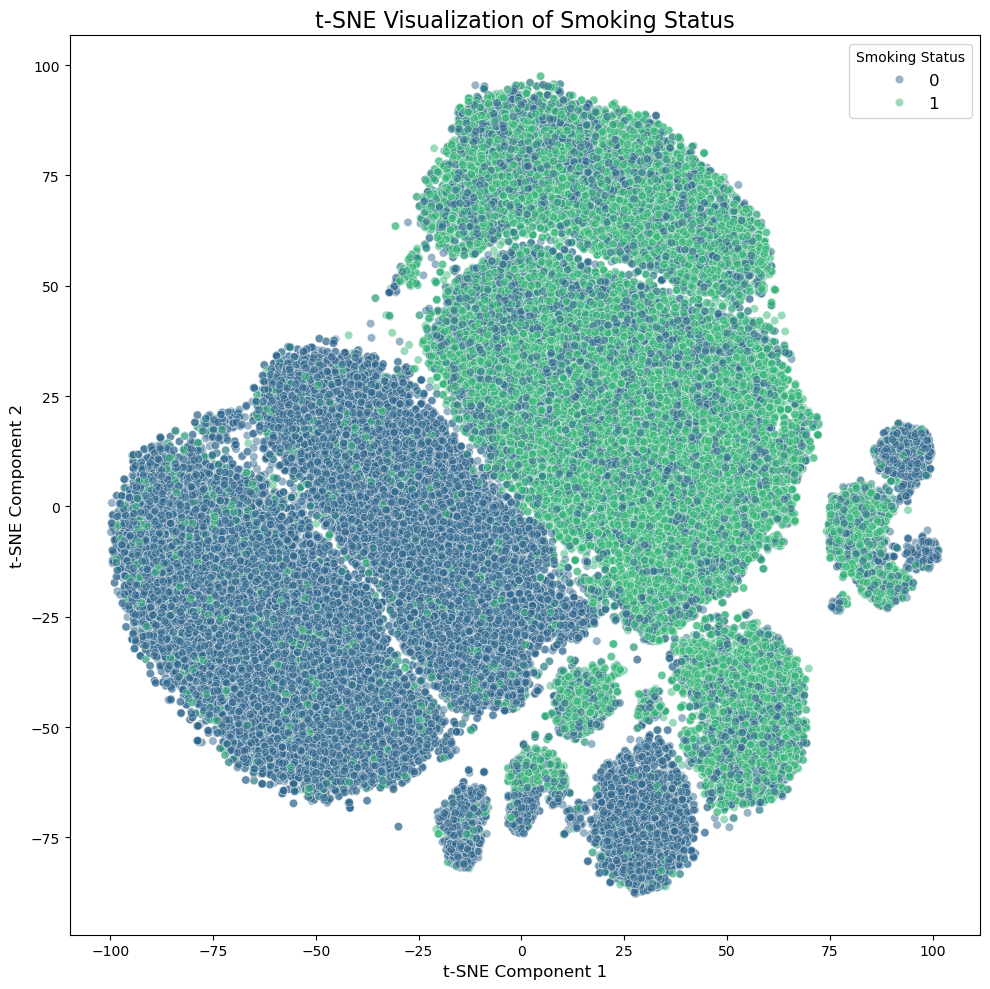
\includegraphics[width=\textwidth]{screen_results/tSNE_smoking_non_smoking.png}
        \caption{t-SNE "Non-fumatore" e "Ex-fumatore o Fumatore"}
    \end{minipage}
    \hfill
    \begin{minipage}{0.45\textwidth}
        \centering
        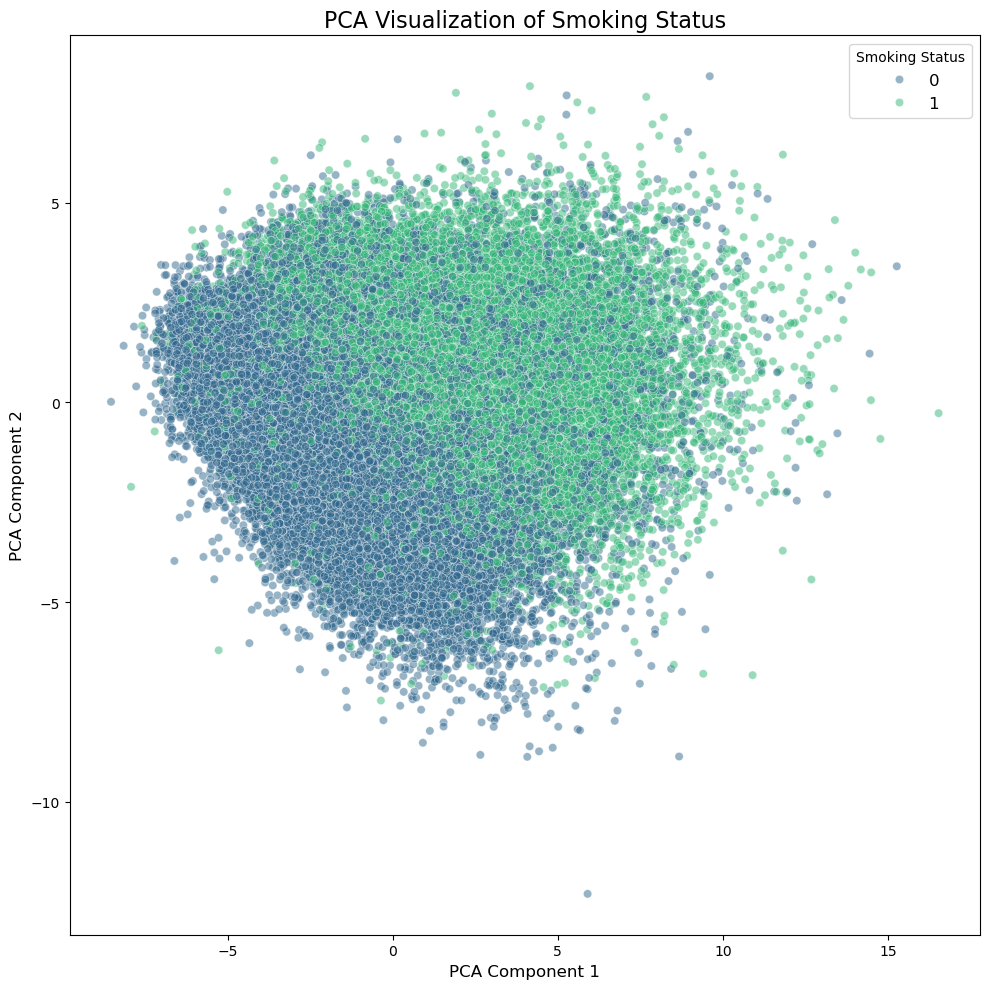
\includegraphics[width=\textwidth]{screen_results/pca_smoking_non_smoking.png}
        \caption{PCA "Non-fumatore" e "Ex-fumatore o Fumatore"}
    \end{minipage}
\end{figure}

\begin{figure}[h]
    \centering
    \begin{minipage}{0.45\textwidth}
        \centering
        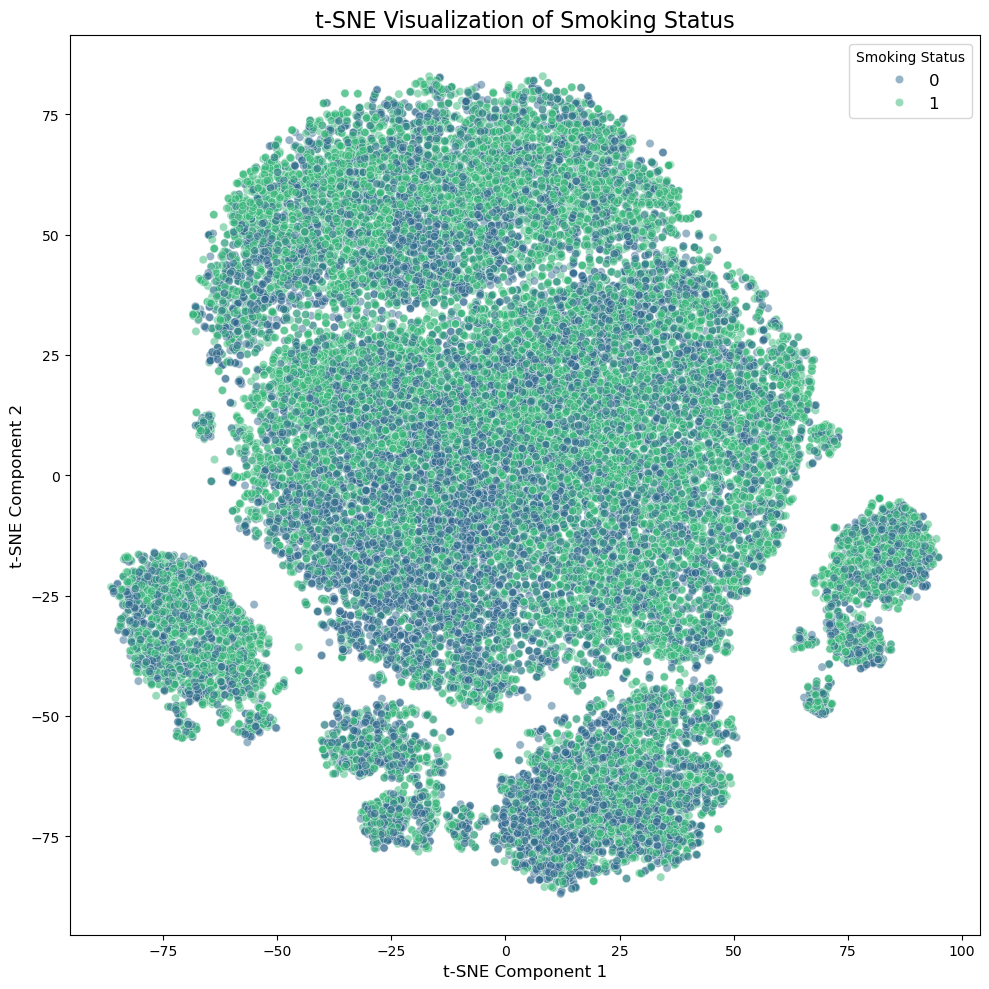
\includegraphics[width=\textwidth]{screen_results/tSNE_smoking_ex_smoking.png}
        \caption{t-SNE "Ex-fumatore" e "Fumatore"}
    \end{minipage}
    \hfill
    \begin{minipage}{0.45\textwidth}
        \centering
        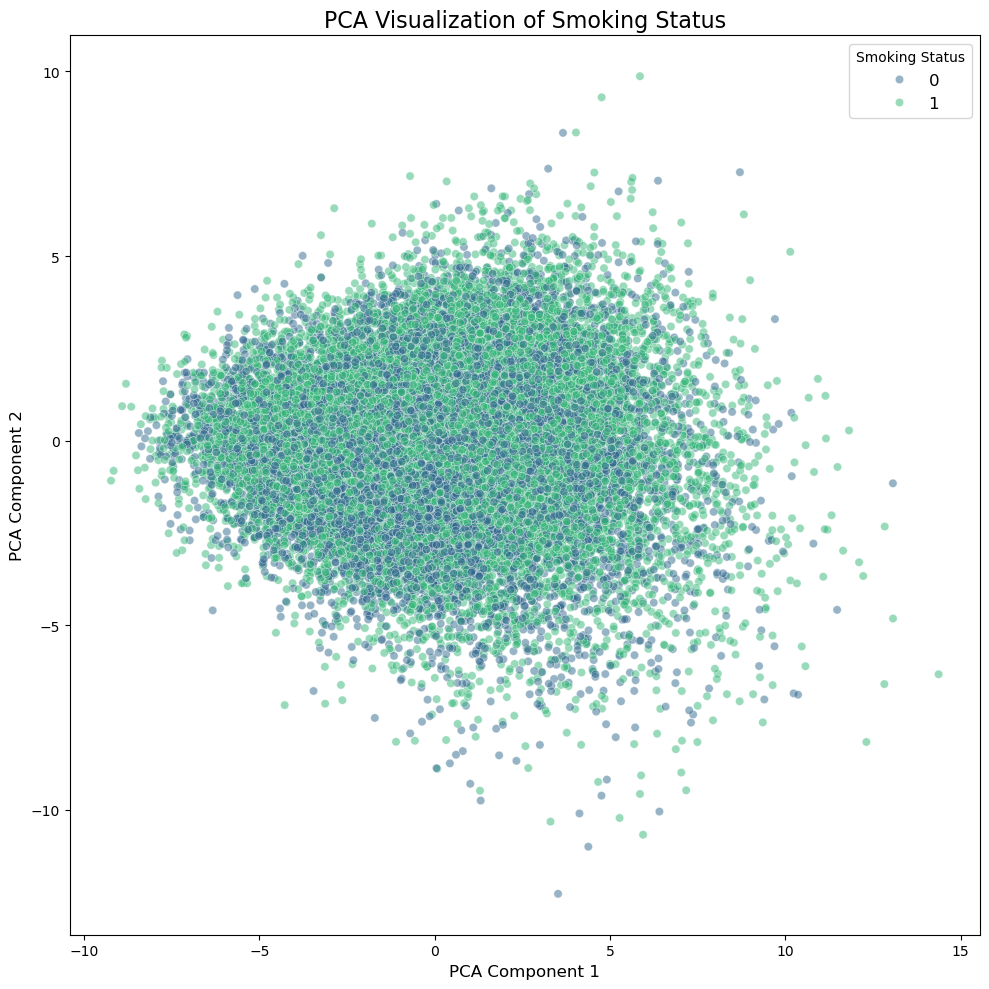
\includegraphics[width=\textwidth]{screen_results/pca_smoking_ex_smoking.png}
        \caption{PCA "Ex-fumatore" e "Fumatore"}
    \end{minipage}
\end{figure}

\begin{multicols}{2}

%%%%%%%%%%%%%%%%%%%%%%%%%%%%%%%%%%%%%%%%%%%%%%%%%%%%%%%%%%%%%%%%%%%%%
\section{Conclusioni}
%%%%%%%%%%%%%%%%%%%%%%%%%%%%%%%%%%%%%%%%%%%%%%%%%%%%%%%%%%%%%%%%%%%%%

I risultati ottenuti in questo progetto, purtroppo non ci hanno soddisfatto pienamente: infatti nonostante l’impiego di modelli avanzati e di diverse tecniche di miglioramento, le metriche finali non hanno mostrato un miglioramento significativo rispetto a quelle ottenute con il modello più semplice utilizzato all’inizio del progetto.

Una delle possibili cause di questa difficoltà potrebbe risiedere nella natura stessa del problema di classificazione affrontato; come già accennato più volte e come si è potuto evincere dall'analisi visiva dei dati tramite t-SNE e PCA, la distinzione tra ex-fumatori e fumatori si è rivelata particolarmente complessa e tutto sommato risulta comprensibile se si considera che la classe degli ex-fumatori è per sua natura "ambigua": il dataset non fornisce informazioni dettagliate riguardo da quanto tempo queste persone abbiano smesso di fumare per esempio.
Inoltre, non è da escludere che alcuni pazienti abbiano fornito dicharazioni false o imprecise riguardo alle proprie abitudini, il che potrebbe aver introdotto degli errori a priori nelle label dei sample.

Inoltre, nonostante fosse pronosticabile che il dataset non fosse per nulla linearmente separabile, tutti i test effettuati hanno evidenziato che molto probabilmente non esista nemmeno una chiara separazione non lineare tra le classi; sebbene quindi siano stati testati svariati modelli predittivi e siano state implementate tecniche avanzate come feature engineering, bagging, stacking e altre strategie di ensemble learning, nessuna di queste ha portato a un incremento significativo delle prestazioni.
Uno dei motivi potrebbe essere che il limite non risiede nei modelli utilizzati, ma nella qualità dei dati: probabilmente nè le feature disponibili nè quelle aggiunte tramite feature egeneering sono sufficientemente rilevanti per poter distinguere in modo netto i tre gruppi e ciò ha quindi reso difficile per qualsiasi modello di Machine Learning individuare pattern chiari.
Un altro motivo potrebbe essere legato alla eterogeneità dei soggetti presenti nel dataset: alcuni individui infatti potrebbero non mostrare anomalie significative nei parametri rappresentati dalle features, pur magari essendo un bevitore o un fumatore abituale, oppure potrebbero essere presenti nel dataset casi patologici di persone con malattie o condizioni particolari che mostrano anomalie in una o più feature, andando cosi ad influenzare la predizione.

A prescindere da queste difficoltà, riteniamo che l’approccio basato sul classificatore gerarchico sia il più sensato per affrontare questo problema, anche se non siamo riusciti a implementarlo esattamente come avevamo previsto: abbiamo comunque ottenuto un primo modello in grado di separare i non fumatori dal gruppo ex-fumatori + fumatori ed idealmente allenando il secondo modello in modo che distingua solo ex-fumatori e fumatori, si potrebbe migliorare ulteriormente la classificazione complessiva.
Come già discusso in precedenza però, per garantire risultati confrontabili con gli altri modelli testati abbiamo dovuto allenare il secondo classificatore su tutte e tre le classi anziché solo sulle due previste nella suddivisione gerarchica ideale.

Nel complesso però la Random Forest si è dimostrata il miglior modello per il nostro problema di classificazione e questo probabilmente grazie alla sua robustezza nei confronti di dati rumorosi, alla sua capacità di gestire feature non lineari e forse anche alla sua natura ensemble che combina più alberi decisionali per ridurre l’overfitting e ottenere previsioni più stabili rispetto ad altri modelli testati. (Results ~\ref{bestmodel_smoke})

Per concludere, questo studio oltre ad aver messo in evidenza la difficoltà intrinseca della classificazione tra fumatori ed ex-fumatori, ha mostrato che in alcuni casi il miglioramento delle prestazioni non può essere raggiunto solo attraverso tecniche più avanzate di Machine Learing, ma richiederebbe dati più dettagliati e informativi.
Sarebbe inoltre necessario testare tecniche di apprendimento più avanzate come le Reti Neurali, che potrebbero essere in grado di individuare pattern complessi che modelli classici di Machine Learning non riescono a cogliere.

%%%%%%%%%%%%%%%%%%%%%%%%%%%%%%%%%%%%%%%%%%%%%%%%%%%%%%%%%%%%%%%%%%%%%
\section*{Bibliografia}
%%%%%%%%%%%%%%%%%%%%%%%%%%%%%%%%%%%%%%%%%%%%%%%%%%%%%%%%%%%%%%%%%%%%%
% Bibliography entries (if any) can be added here.
\printbibliography[heading=none]

\end{multicols}
\end{document}


